\documentclass[12pt,a4paper]{report}

\usepackage{graphics}
%\usepackage{fullpage,epsf,graphicx, amstext,url} 
%\usepackage{epsf}
\usepackage{graphicx}
\usepackage{amstext}
\usepackage{url}
\usepackage{amssymb}
\usepackage{graphicx}
\usepackage{amsmath}

%\graphicspath{ {/home/george/Desktop/Tex_Dissertation/images} }
%
% head.sty is no longer needed
%
%\usepackage{head,fullpage,epsf,graphicx, amstext,url} 

\def\BibTeX{{\rm B\kern-.05em{\sc i\kern-.025em b}\kern-.08em
    T\kern-.1667em\lower.7ex\hbox{E}\kern-.125emX}}

\begin{document}

\thispagestyle{empty}

%                       This is a basic LaTeX Template
%                       for the MSc Dissertation report
%
\parindent=10pt          %  Switch off indent of paragraphs 
\parskip=5pt            %  Put 5pt between each paragraph  
%
%                       This section generates a title page
%                       Edit only the sections indicated to put
%                       in the project title, and submission date
%

\vspace*{0.1\textheight}

\begin{center}
        \huge{\bfseries Calculation of the Supersymmetric top quark mass at CLIC}\\
\end{center}

\bigskip

\begin{center}
        \large{Georgios Billis}\\      % Replace with your name
        \bigskip
        \large{August 18, 2017}        % Submission Date
\end{center}

%%% If necessary, reduce the number 0.4 below so the University Crest
%%% and the words below it fit on the page.
%%% Don't let the crest and the wording below it flow onto the next page!
\vspace*{0.35\textheight}

\begin{center}
        
\includegraphics[width=35mm]{crest.pdf}
\end{center}

\medskip

\begin{center}

%%%
%%% Change Theoretical to Mathematical if appropriate
%%%
\large{
  MSc in Theoretical Physics\\[0.8ex]
  The University of Edinburgh\\[0.8ex]
  2017
}

\end{center}

\newpage


\pagenumbering{roman}

\begin{abstract}
In this project I calculate the mass of the Supersymmetric top quark in CLIC experiment at $\sqrt{s}$ = 3 TeV in $e^{-}$ $e^{+}$ collisions. I assume the following decay for the top squark $\tilde{q} \rightarrow q$ $\chi_{0}$, 
and I focus on the fully hadronic channel of decay i.e $\tilde{q} \rightarrow q$ $\chi_{0} \rightarrow$ $W b \tilde{\chi}_{1}^{0}$ .
The mass was found  to be  $m_{\tilde{t}}$ = 861 $\pm$ 19 GeV using the Boosted Descision 
Trees Multivariate Analysis and $m_{\tilde{t}}$ = 812 $\pm$ 20 GeV using the Gradient Boosted Descision  Trees Multivariate Analysis. 
\end{abstract}

\pagenumbering{roman}


\textbf{Declaration}


\newpage

\tableofcontents
\listoftables
\listoffigures

\begin{titlepage}
\vspace*{2in}
% an acknowledgements section is completely optional but if you decide
% not to include it you should still include an empty {titlepage}
% environment as this initialises things like section and page numbering.
\section*{Acknowledgements}

Put your acknowledgements here. Thanking your supervisor for his/her
help is standard practice, but you don't have to do this\ldots

This template is is modification of the one for the MSc in High
Performance Computing, which is apparently descended from a template
developed by Prof Charles Duncan for MSc students in Meteorology. His
acknowledgement follows:

\emph{This template has been produced with help from many former
  students who have shown different ways of doing things. Please make
  suggestions for further improvements.}

Some parts of this template were lifted unashamedly from the Edinburgh
MPhys project report guide, with little or no modification. I have no
idea who wrote the first version of that\ldots

You don't have to use \LaTeX\ for your dissertation. You can use
Microsoft Word or Apple Pages if you wish, but it's \emph{much} easier
to typeset equations in \LaTeX, and references look after
themselves. Whatever you use, your dissertation should have the same
general structure, and it should look similar to this one --
especially the front page.


\end{titlepage}

\pagenumbering{arabic}

\chapter{Introduction}

On July 2012 the discovery of the Higgs boson was announced at CERN's Large Hadron Collider (LHC). This marked the begining of a new era for experimental High Energy Physics motivating the design of new 
experiments for further and deeper exploration of the Higgs boson itself but also, a huge marathon
addressing the questions/problems that arose with it. 

One of these proposed experiments is Compact Linear Collider (CLIC), a high-luminosity linear $e^{-}$ $e^{+}$ collider. It is designed for a staging scenario of three main centre of mass energies at $\surd{s}$ = 380 GeV, $\surd{s}$ = 1.5 TeV
and $\surd{s}$ = 3 TeV targeting optimal physics output based on the current landscape. The main difference of CLIC with LHC is that in the latter, protons collide which are non fundamental particles as they consist of quarks and 
gluons bound alltogether. One of the disadvantages of LHC is the inability to know beforehand the initial state of the colliding particles as quarks exist in a "sea of gluons" making it impossible to know their momenta. This sets
some restrictions with resprect to the precision that it can probe various observables.

On the other hand, CLIC is designed to invastigate the interactions of elementary particles, an important advantage since initial states of the colliding particles is known. In advance, LHC suffers from energy loss due to 
Synchrotron radiation since protons are accelerated in a 27 km circular accelerator whereas CLIC, being linear does not.

The main targets of CLIC are dependent of the energy stage. In the first it will focus on prescision standard model physics such as Higgs and Top quark measurements and in the two subsequent, among others, there will be searches
for new physics~\cite{clic2016updated}. One of the theories that aspires to give solutions to many of the problems of Standard Model is Supersymmetry (SUSY). In this theory every particle has a Supersymmetric partner that differs in the spin by $1/2$, thus 
relating bosons with fermions and fermions with bosons.

In the Minimal Supersymmetric Standard Model, the top squarks $\tilde{t}$ decay almost all the times into a top quark $t$
and a dark matter candidate, the neutralino $\tilde{\chi}_{1}^{0}$. In this project I will use Multivariate Analisis
to discriminate the best it can be achieved between signal and background with the goal to measure the top squark
mass at $\surd{s}$ = 3 TeV in the CLIC accelerator environment.






\chapter{CLIC}

\section{Outline of the experiment}

CLIC is a proposed $e^{-}$ $e^{+}$ linear collider optimised to perform in three centre of mass stages at 
$\surd s$ = 380 GeV, $\surd s$ = 1.5 TeV and $\surd s$ = 3 TeV. The purpose of the different energy stages is to 
fully exploit its scientific potential including precision measurements and searches for physics Beyond the 
Standar Model.

Specifically, at $\surd s$ = 380 GeV and with an integrated luminosity of $\mathcal{L}_{int}$ = 500 fb$^{-1}$, 
prescision measurements can be made in the Higgs and the top quark sector. At this enegy stage the Higgsstrahlung
process ($e^{+}e^{-}\rightarrow ZH$) alongside the $WW$ fusion ($e^{+}e^{-}\rightarrow H\nu_{e}\tilde{\nu}_{e}$) 
are the dominant and can shed light to properties of the Higgs boson in a model independent way~\cite{clic2016updated}.
In CLIC there is also a dedicated program for top quark physics, as it is one of the most important particles
in SM because it couples strongest to the Higgs field due to its mass but also it has an important role in 
many of the BSM scenarios.
Furthermore at the next two stages leading role will play the proposed scenarios for physics BSM with most 
importantly Supersymmetry at $\surd s$ = 3 TeV and with $\mathcal{L}_{int}$ = 2000 fb$^{-1}$. This  is because CLIC has the potential for direct particle detection up to the 
kinematic limit of $\surd s /2$ for pair production but also through indirect detection of observables that are sensitive to BSM
scenarios through precision measurements and comparison with the SM expectations, 
taking advantage of the full energy potential.



Given the linear nature of CLIC, there are no energy losses induced by Synchrotron radiation which appears in 
circular colliders, but due Beamsstrahlung radiation. As the colsliding bunches get closer to the 
vertex, the strong electromagnetic fields (up to 10 Tesla) created by the opposing beam, cause deflection
of the partices trajectories resulting to emit Synchrotron radiation. The effect is energy-dependent with huge
impact at higher energies~\cite{bonvicini1989first} as it can be seen in the following 
image~\cite{abramowicz2017higgs}.

\begin{figure}[h!]
  \centering
  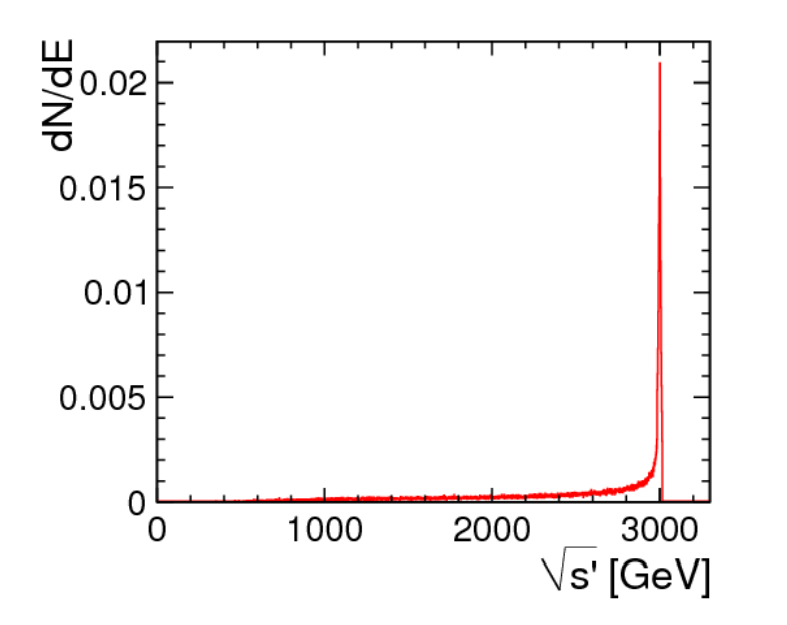
\includegraphics[width=0.7\linewidth]{{images/beamsstrahlung}.png}
  \caption{\scriptsize{The luminosity spectrum for CLIC operating at $\surd s$ = 3 TeV, where $\surd s'$ is the
  effective centre-of-mass energy after beamstrahlung and initial state radiation.}}
  \label{fig2.15}
\end{figure}

CLIC is designed to operate for seven, five and six years respectively in each energy stage while the 
upgrading periods will last two years. The total run will last for 22 years with the following table summarising
the luminosities achieved in each stage:

\begin{table}[h]

\centering % used for centering table
\begin{tabular}{c c} % centered columns (4 columns)
\hline %inserts double horizontal lines
$\surd s$ (GeV)  & $\mathcal{L}$   \\ \hline % inserts single horizontal line
380 & 500 fb$^{-1}$  \\
1.5 & 1.5 ab$^{-1}$ \\
3   &  3 ab$^{-1}$ 
 %inserts single line
\end{tabular}
\label{table:nonlin} % is used to refer this table in the text
\end{table}

Furthermore, the experiment has two detector concepts CLIC SiD and CLIC ILD in order to serve the required 
jet energy resolution. The latter has been  developed for the International Linear Collinder but it has been
adapted according to the needs of CLIC. Both detectors have strong central solenoid magnets creating an axial 
magnetic field of 5T for CLIC SiD and 4T for CLI ILD~\cite{abramowicz2017higgs}.



\chapter{Supersymmetry}

\section{Motivation}

The model that describes elementary particle physics is the Standar Model. It involves matter  fields (fermions)
and vector gauge bosons (force carriers) that they stem from the fact that the SM Lagrngian is subject to $SU(3) \otimes 
SU(2) \otimes U(1)$ symmetries. An important part of this theory is the existence of the Higgs field which appeared
during the unification of the electromagnetic and the weak force. It is known for the fact that it "gives"
mass to the elementary particles (besides photons and gluons which they are protected by the $U(1)$,$SU(3)$
symmetries respectively)
via Spontaneous Symmetry Breaking .

It is true that even with the great success that the SM has been probed does not consist a flawless theory.
Many parts of it are still to be answered or contain significant controversies. One example is the Hierarchy 
problem. In the electroweak sector of the SM there is a parameter that has the dimensions of energy, the 
vacum expectation value of the Higgs field which phenomenologicaly is 

\begin{equation}
 \upsilon \approx 246 \quad GeV
\end{equation}

The importance of this parameter is that it sets the masses of the the theory and as well as the Higgs boson
itself as it is

\begin{equation}
 M_{H} = \upsilon \sqrt{\frac{\lambda}{2}} 
\end{equation}


where $\lambda$ is the constant of the Higgs self interaction. The problem arises when we try compute higher 
order corrections to the mass of the Higgs field. The self energy of the higgs boson has a term of the form

\begin{equation}
 \int_{}^{\Lambda} d^{4}k \quad f(k,external\quad momenta)
\end{equation}

where $\Lambda$ represents the scale of the new physics such as the effects of quantum gravity. In dimensional 
regularisation, when $\Lambda \rightarrow \infty$ the renormalisability of the theory assures that there
is no inconsistency, but if we take into account a scale, for example, for the quantum gravity then $\Lambda \rightarrow 
M_{P} \approx 1.2\times 10^{19}\quad GeV$ which is the Plank mass, then the additive quantum corrections for the Higgs 
mass become too big dragging the value of the Higgs mass up. Because the VEV of the Higgs boson has a fixed 
phenomenologicaly value, one way to circumvent this problem is by relating bosons with fermions since in the 
latter, the algebraic terms for their self energies come with a minus sign giving the desired calcelations 
without any "fine tuning" from our side. This results into the SUSY theory stabilising the Hierarchy $M_{H}
\ll M_{P}$ with the constraint that the SUSY particles should be visible at a scale not too much greater 
than 1-10 TeV~\cite{aitchison2005supersymmetry}.

One other feature that makes SUSY attractive is the fact that it includes the convergence of the couplings,
something that it is known as Grand Unification. From the point of view of SM, something like that is 
unable to achieve since two of the couplings decrease with energy (weak and strong coupling) whereas one
(electromagnetic) increases. In the MSSM, by the inclusion of the sparticles such unification is actually
achievable as it can be seen in the following figure:

\begin{figure}[h!]
  \centering
  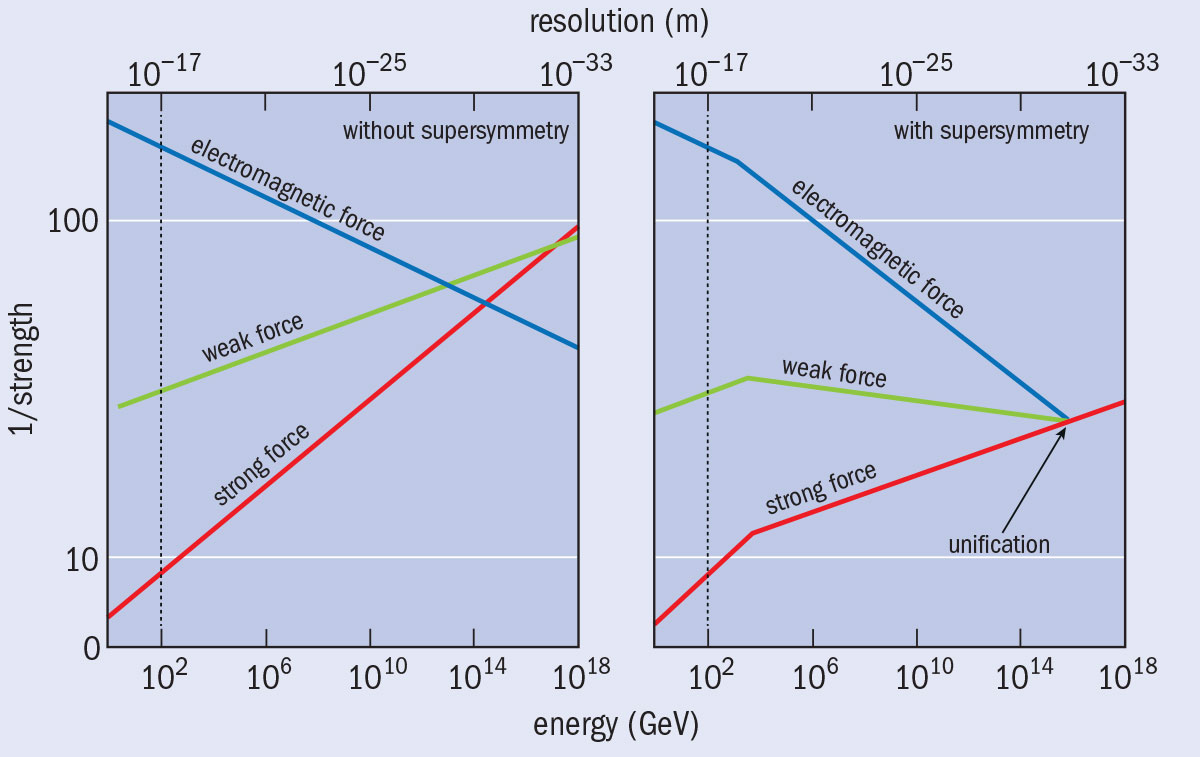
\includegraphics[width=0.7\linewidth]{{images/PWOct14gates-fig2-full}.jpg}
  \label{}
\end{figure}



\section{SUSY Phenomenology}

Inside SUSY every boson is related to a fermionic supersymmetric partner and every fermion has a bosonic one. The 
fermion superpartners are called sfermions and differ in the spin value by 1/2 whereas the boson particles 
which are the force carries are related to a spin 1/2 particles, the gauginos. In the following table I show
the correspondance between SM and SUSY gauge particles.

\begin{table}[ht]

\centering % used for centering table
\begin{tabular}{c c c c} % centered columns (4 columns)
\hline\hline %inserts double horizontal lines
Standard Model  &  & SUSY &  \\ [0.5ex] 
\hline % inserts single horizontal line
Photon & $\gamma$ & Photino & $\tilde{\gamma}$ \\ % inserting body of the table
Gluon & g & Gluino & $\tilde{g}$ \\
Z Boson & Z & Zino & $\tilde{Z}$ \\
W Boson & $W^{\pm,0}$ & Wino & $\tilde{W}^{\pm,0}$ \\
B Boson& B & Bino & $\tilde{B}$ \\ [1ex] % [1ex] adds vertical space
\hline %inserts single line
\end{tabular}
\label{table:nonlin} % is used to refer this table in the text
\end{table}

The framework of this project is the Minimal Supersymmetric Standard Model which besides the SM particles 
includes the sleptons $\tilde{\ell}^{\pm}$, the sneutrinos $\tilde{\nu}_{l}$, the squarks $\tilde{q}$, the 
gluinos $\tilde{g}$, two pair of charginos $\tilde{\chi}^{\pm}_{i}$ where $i=1,2$,  four neutralinos 
$\tilde{\chi}^{0}_{i}$, $i=1,...,4$ and five Higgs bosons $h^{0}$, $H^{0}$, $A^{0}$,$H^{\pm}$.

Both particles and sparticles belong to the same super-multiplet having the same mass and the same quantum 
numbers as their SM partners but with different spin. Because no such degenerate fermion-boson pair exists 
in nature,
then it is deduced that SUSY must be a broken symmetry. In order to constitute a solid solution to the 
Hierarchy problem, then the difference in the masses of the particles and their supersymmetric partners 
must be of the order of $\mathcal{O}(1  TeV) $~\cite{nagashima2014beyond}.

In Standard Model, for the Spontaneous Symmetry Breaking one Higgs doublet is needed with 4 degrees of 
freedom. For the SUSY model on the other hand two such doublets are required with a total of eight 
degrees of freedom where three of them are absorbed to give mass to the SM particles such as W$^{\pm}$ and Z,
and the remaining five give rise to five physical Higgs bosons $\tilde{h}$,$\tilde{H}^{\pm}$,$\tilde{A}$,
$\tilde{H}^{0}$. Those in turn, mix further to become the neutralinos and the charginos : $\tilde{\chi}_{i}^{0}$,
$\tilde{\chi}_{i}^{\pm}$. 

It is known that within the SM the fermions carry chirality denoted by L or R whether they are left or right 
respectively, according to the way they transform under the symmetry group $SU(2) \otimes U(1)$. Thus given 
the SUSY relation of fermions-bosons that means that the sfermions  (bosonic superpartners), come into 
doublets of the form $(f_{i},\tilde{f}_{i})$, where i=L,R. The sfermions mix further to make the eigenstates
of the mass matrix. This mixing is expected to be strong for third generation sfermions since the Yukawa 
couplings can be large, more precisely in our case the stop quark mixing effects can be large because
of the large mass of the top quark.

The following matrix is the mixing matrix expressed in the $(\tilde{f}_{L},\tilde{f}_{R})$ basis:

\begin{equation}
 \mathcal{M}^{2}_{\tilde{f}} =

 \[  
  \begin{pmatrix}
   M^{2}_{\tilde{f}_{L}}  &  \alpha_{f}m_{f} \\
   \alpha_{f}m_{f}        &  M^{2}_{\tilde{f}_{R}}
  \end{pmatrix}
\]
\end{equation}

where the $M^{2}_{\tilde{f}_{L}}$ are terms that depend on the mass of the quark, the charge and the third 
component of the weak isospin. The off diagonal elements $\alpha_{f}$ are dependent on the soft SUSY breaking
trilinear scalar coupling parameters.

In this project I will focous on the top squarks  where the mixing   $\tilde{t}_{R}-\tilde{t}_{L}$ is important
due to the large top quark mass. By computing the eigenvalues of the previous matrix and for the right
flavour we obtain:

\begin{equation}
 m^{2}_{\tilde{t}_{1,2}} = \frac{1}{2}(M^{2}_{\tilde{t}_{L}} + M^{2}_{\tilde{t}_{R}} \mp 
 \sqrt{(M^{2}_{\tilde{t}_{L}}-M^{2}_{\tilde{t}_{R}})^{2} + 4 m^{2}_{t}\alpha^{2}_{t}})
\end{equation}

It is obvious that the $m^{2}_{\tilde{t}_{1}}$ will have the lowest mass, something that makes it the 
lightest squark.

\section{Results from LHC for SUSY}
 
 The search for indications for Supersymmetry is not new as LHC has been optimized and focused among other
 to the direct or indirect detection of sparticles. The majority of the cases that have been studied, 
 consider as main decay channel of the sparticles the following:
 
 \begin{equation}
  BR(\tilde{q} \rightarrow q  \chi_{i}^{0,\pm}) = 100 \%
 \end{equation}

So far thought no indication of SUSY has been found in LHC but through each analysis the exclusion limits 
for the SUSY observables become bigger and bigger as it can be seen in the following figures that summarises
the latest of them for the stop quark mass at $\surd s$ = 8,13 GeV in proton proton collisions
~\cite{aaboud2016search}:

\begin{figure}[h!]
  \centering
  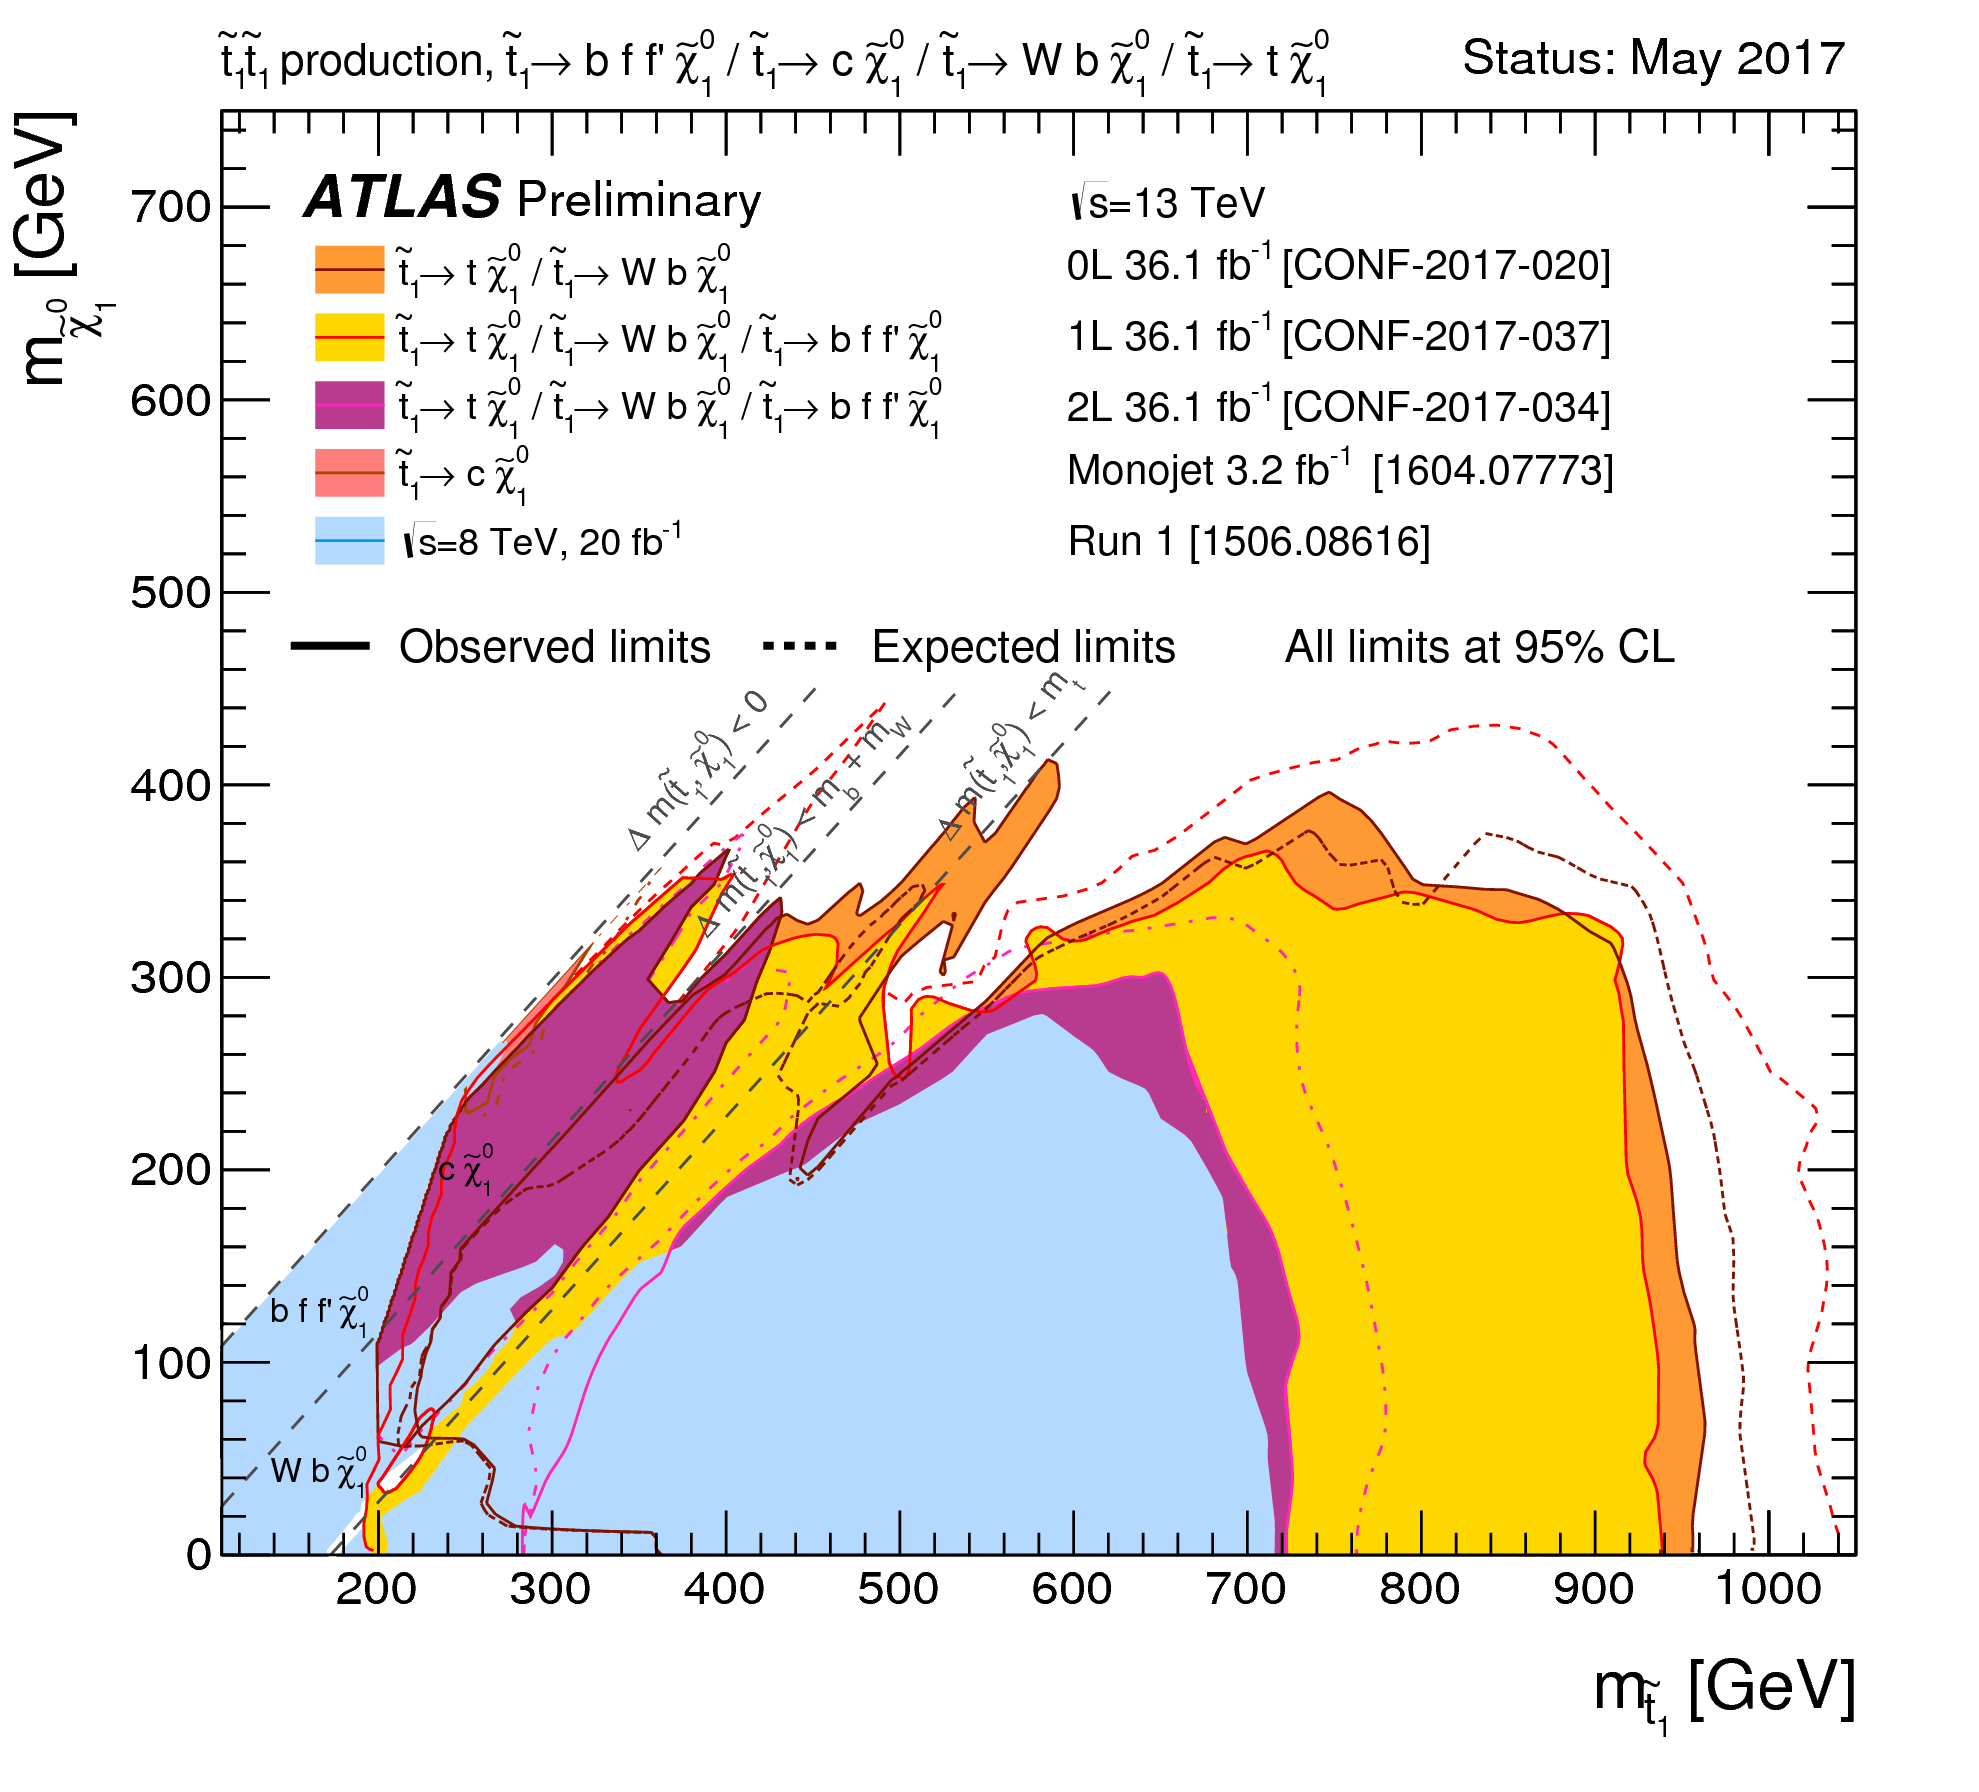
\includegraphics[width=0.7\linewidth]{{images/ATLAS_SUSY_Stop_tLSP}.png}
  \label{fig2.15}
\end{figure}

Whereas in the following figure there are the exclusion limits in ATLAS for p-p collisions at 13 TeV for the
channel invastiged in this project

\begin{figure}[ht!]
  \centering
  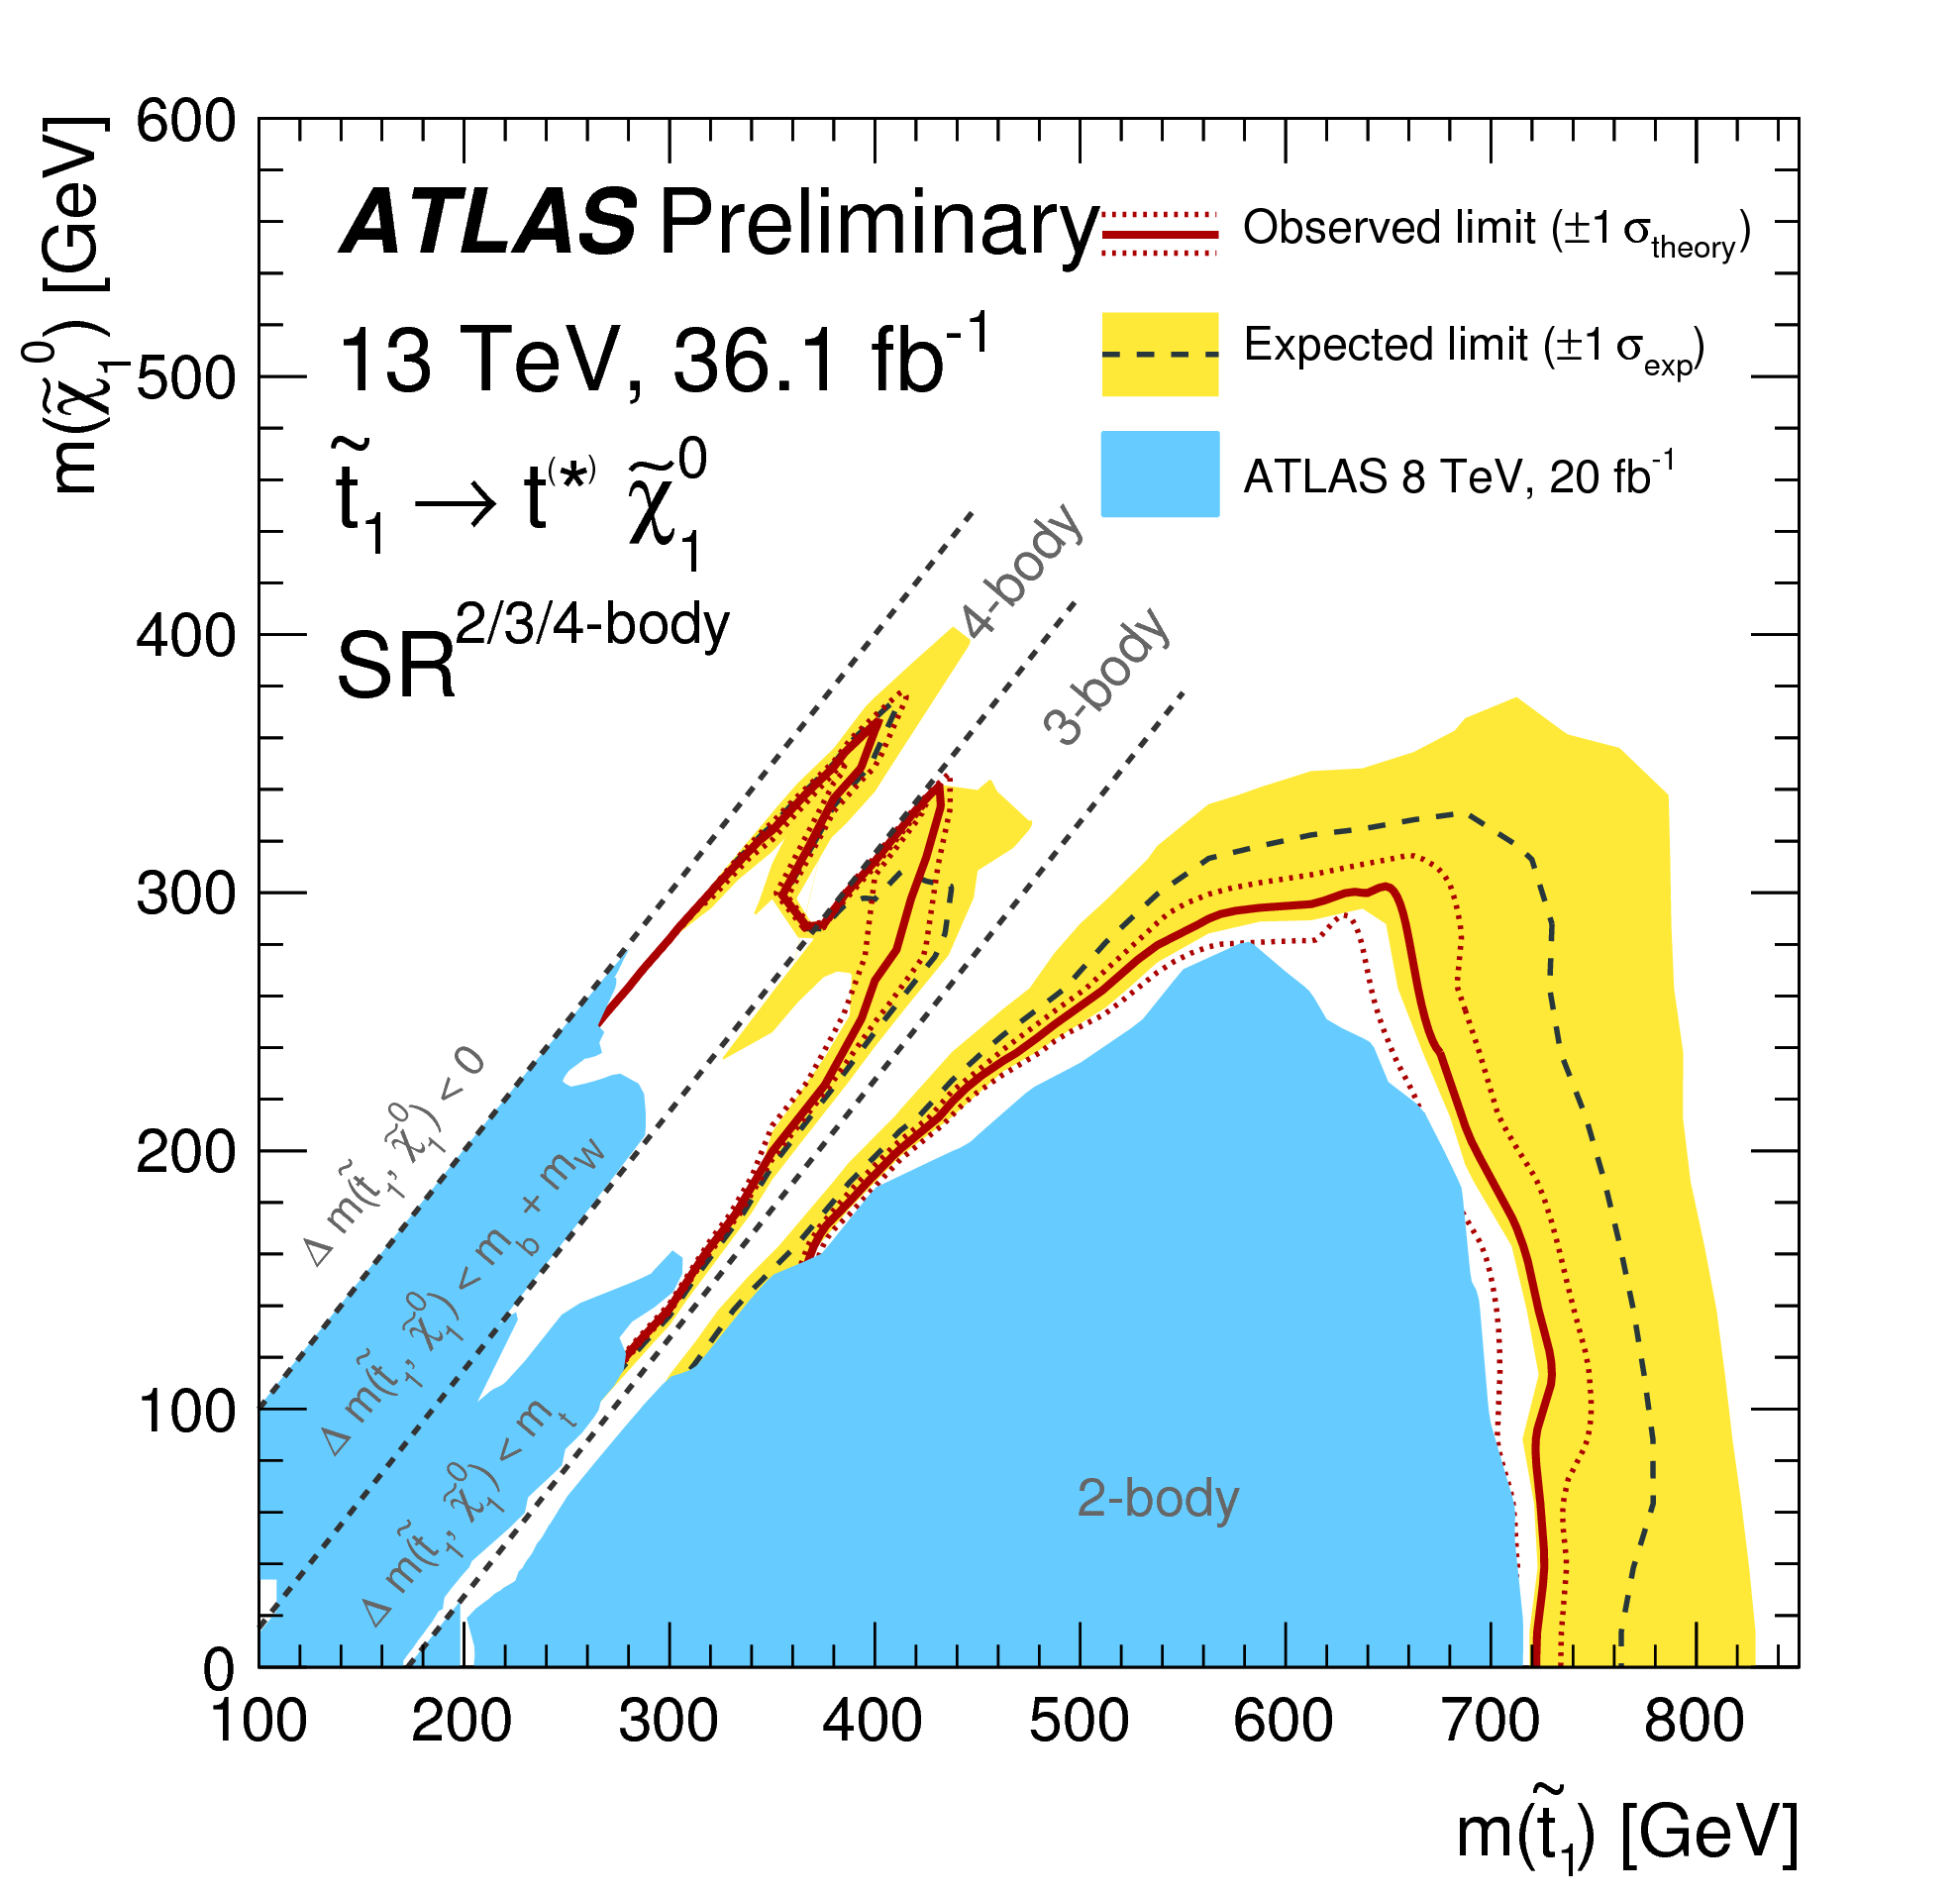
\includegraphics[width=0.6\linewidth, scale=5]{{images/fig_08}.png}
  \label{}
\end{figure}






\chapter{Methods}
\section{Introduction}

In this chapter I will describe the exact conditions and methods that were followed in this project for the 
calculation of the stop quark mass at CLIC Conceptual experiment.

I will invedtigate the production of a pair of stop quarks at $\surd s$ = 3 TeV and assumig an  integrated 
luminosity of $\mathcal{L}_{int}$ = 2000 fb$^{-1}$. The channel of interest is the following:

\begin{equation}
 e^{+} e^{+} \rightarrow \tilde{t} \tilde{\bar{t}} \rightarrow t\tilde{\chi}_{1}^{0} \bar{t}\tilde{\chi}_{1}^{0}
 \rightarrow W^{+}W^{-}b\bar{b} \tilde{\chi}_{1}^{0} \tilde{\chi}_{1}^{0}
\end{equation}

and for this model the mass of the top squark is $m_{\tilde{t}}$ = 844 GeV whereas the mass of the 
neutralino is $m_{\tilde{\chi}_{1}^{0}}$. This is not the only possible decay of a top squark but it is the
dominant one. In what follows I show the top three branching ratios of the top squark decay and two
of the corresponding Feynmann diagrams:

\begin{figure}[ht!]
  \raggedleft
  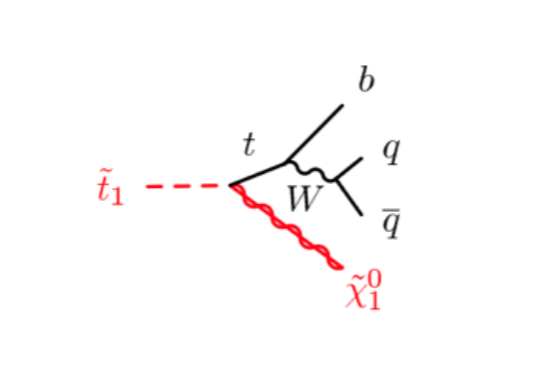
\includegraphics[width=0.4\linewidth]{{images/feyn1}.png}
  \hspace{\fill}
    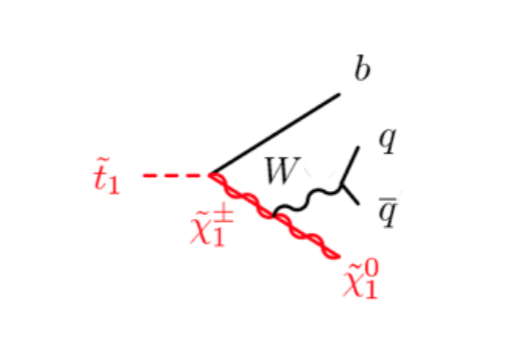
\includegraphics[width=0.4\linewidth]{{images/feyn2}.png}
  \label{}
\end{figure}


\newpage

\begin{enumerate}
 \item BR($\tilde{t}\rightarrow t \tilde{\chi}_{1}^{0}$) = 52.4 \%
 \item BR($\tilde{t}\rightarrow b \tilde{\chi}_{1}^{\pm}$) = 34.1 \%
 \item BR($\tilde{t}\rightarrow t \tilde{\chi}_{2}^{0}$) = 13.2 \%
 \end{enumerate}

As also the branching ratios for the decay of the W boson to either in a hadronic final state or in
a leptonic one are:

\begin{itemize}
 \item BR($W\rightarrow q\bar{q}$) = 67.8 \% 
 \item BR($W\rightarrow l\nu_{l}$) = 32.2 \%
\end{itemize}

In the following I summarise the possible decays of the stops indicating the branching pair fraction
for each one:

\begin{itemize}
 \item $e^{-}e^{+} \rightarrow \tilde{t}\tilde{\bar{t}} \rightarrow t \tilde{\chi}_{1}^{0}
 \chi^{\pm}_{1}b \rightarrow
 W^{+}W^{-} b \bar{b} \tilde{\chi}_{1}^{0}  \tilde{\chi}_{1}^{0}$ \quad (35.8\%)

 \item $e^{-}e^{+} \rightarrow \tilde{t}\tilde{\bar{t}} \rightarrow t\bar{t} \tilde{\chi}_{1}^{0}
 \tilde{\chi}^{0}_{1} \rightarrow
 W^{+}W^{-} b \bar{b} \tilde{\chi}_{1}^{0}  \tilde{\chi}_{1}^{0}$ \quad (27.4\%)

 \item $e^{-}e^{+} \rightarrow \tilde{t}\tilde{\bar{t}} \rightarrow t\bar{t} \tilde{\chi}_{1}^{0}
 \chi^{0}_{2} \rightarrow
 W^{+}W^{-} b \bar{b} \tilde{\chi}_{1}^{0}  \tilde{\chi}_{1}^{0}h$ \quad (13.7\%)
 
 \item $e^{-}e^{+} \rightarrow \tilde{t}\tilde{\bar{t}} \rightarrow b\bar{b} \chi_{1}^{+}
 \chi^{-}_{1} \rightarrow
 W^{+}W^{-} b \bar{b} \tilde{\chi}_{1}^{0}  \tilde{\chi}_{1}^{0}$ \quad (11.6\%)
 
 \item $e^{-}e^{+} \rightarrow \tilde{t}\tilde{\bar{t}} \rightarrow t \tilde{\chi}_{2}^{0}
 \chi^{\pm}_{1}b \rightarrow
 W^{+}W^{-} b \bar{b} \tilde{\chi}_{1}^{0}  \tilde{\chi}_{1}^{0}h$ \quad (9\%)
 
 \end{itemize}


\newpage

\section{Calculation of SUSY particle masses}

There are various ways that have been developed for the calculation of the squark masses at electron-positron
linear colliders. In this chapter I present one that will not be used in my analysis but sketch the potencial
and thus the importance of the aforementioned colliders regarding these kind of calculations.

The main topologies that are considered are those that the gluino is heavier than the squarks and thus the 
dominant decaying channel is:

\begin{equation}
 e^{-}e^{+} \rightarrow \tilde{q} \tilde{\bar{q}} \rightarrow q\bar{q}\chi_{1}^{0}\chi_{1}^{0}
\end{equation}

It needs to be mentioned that a powerfull advantage of the CLIC experiment is the possibility of achieving 
polarisation up to 80$\%$ helping to reduce the WW background and the ability to create right or left squarks
depending on the needs of the physical analysis.

\subsection{Modified Invariant Mass}

This technique has been developed initially for LHC experiment where the p-p collision energy is not known.
The calculation was achieved by creating the variable $M_{C}$ which is related to the standard 
invariant mass but it's invariance comes from contra linear boosts of equal magnitude. The squark mass is given
by:

\begin{equation}
 m_{\tilde{q}}=\frac{1}{2} \big(M_{C}^{max} + \sqrt{(M_{C}^{max})^{2} + 4m_{\chi}^{2}} \big)
\end{equation}

where 

\begin{equation}
 M_{C}^{2}=2(E_{q,1}E_{q,2}+\vec{p}_{q,1}\vec{p}_{q,2})
\end{equation}

and

\begin{equation}
 M_{C}^{max}=\frac{m^{2}_{\tilde{q}}-m^{2}_{\chi}}{m_{\tilde{q}}}
\end{equation}

The power off this kind of calculation comes from the fact that no knowledge for the exact center of mass 
energy is needed (In comparison with the first method described in~\cite{simon2010techniques}), something that is not purely known since the effects of initial state radiation and
the Beamstrahlung can distort it significantly resulting to even bigger uncertainties. Note that this method 
assumes that the mass of the neutralino is known and that the quark is massless. 

\section{Minimisaton of $\chi^{2}$ Method}

In this chapter I describe the procedure that I followed until the calculation of the top squark mass. 
This involved the vertex finding, the jet clustering, the flavourtagging and the calculation of the $\chi^{2}$
for each top squark mass.

\subsection{Vertex Finding}

For the needs of this projecct I used the package of LCFIplus which is an improved software of the already 
existing one LCFIVertex. The important difference between the  two is that LCFIplus employs the vertex finding 
befere the jet clustering (in comparison to LCFIVertex which follows the exact oposite procedure) with the 
goal to protect the secondadry vertices from breaking up and grouped into different jets~\cite{suehara2016lcfiplus}.
This is an important step towards better performance since the Bottom jets can be identified from their 
sufficiently large distance between the primary vertex and their decay vertex. Additionally, the importance
of this step to be performed before jet clustering, is that hadrons that contain bottom or charm quarks 
have sizeable lifetimes and they can be measured Inside the detector.


That said, the vertex finding was the first step towards obtaining the final data for analysis.

\subsection{Jet Clustering}

Jets are an indespensible part of high energy physics. They come from the manifestation of strong nuclear
as free quarks or gluons hadronize. They are visual structures that are measured in the detectors and they
serve the need of approaching the initial parton that they originated. Throught the years various algorithms 
have been developed for the clustering of such objects differing in the way that the approach suchh procedure.
Two of the most famous are the sequential recombination algorithms and cone algorithms. In this projecct I use
the a sequential recombination algorithm, the $k_{t}$ algorithm which is a longitudinaly invariant algorithm
firstly designed for hadron colliders.

The $k_{t}$ involves a measure of distance $d_{ij}$ for all the pair of particles $i,j$:

\begin{equation}
 d_{ij}=d_{ji}=min(p_{Ti}^{2},p_{Tj}^{2})\frac{\Delta R^{2}_{ij}}{R^{2}}
\end{equation}


where $p_{Ti}$ is the transverse momentum of $i^{th}$ particle with respect to beam direction and 
$\Delta R^{2}_{ij}=(y_{i}-y_{j})^{2}+(\phi_{i}-\phi_{j})^{2}$ with $y$ being the rapitdity, $\phi$ being
the azimuth angle and R the jet radius fixed in this project as $R=0.7$.

The basic idea behind this algorithm is that it calculates the $d_{ij}$ with the smallest value and then it 
"merges" the $i,j$ into a single object with momentum $p_{i}+p_{j}$. This procedure is repeated until the quantity
$d_{ij}$ is above some threshold and all the particles that are left are the event's jet
~\cite{cacciari2012fastjet}.

\subsection{Flavour Tagging}

Flavour Tagging is the procedure in which a pseudoprobability is assigned to each jet regarding the parton
that the jet originates from. In this project, there are six jets in the final products four of them 
originating from b quarks. 

The flavour tagging algorithm that was used belonged in the LCFIplus package~\cite{suehara2016lcfiplus}.
It  makes use of the TMVA package which in turn uses multivariate classifiers. A set of input variables are 
defined for each jet and they are passed to the Gradien Boosted Descision Trees (a certain type of classifiers)
which they are trained and then applied to the jets of the physical process. Those input variables are
constituents of the jets such as tracks and secondary vertices.

\subsection{Classification Method: \textit{Boosted Descision Trees}}

For the calculation of the top squark mass I made use of the TMVA package wich is provides a multivariate 
analysis platform in order (for this project) to make separation between the signal and the background. Two 
of them were empoyed, used and compaired: the \textit{Boosted Descision Trees} (BDT) and the 
\textit{Gradient Boosted Descision Trees} (GBDT).

In this chapter I describe the Boosted Descision Trees method of classification and cite the results of this 
investigation.

\subsubsection{Background on BDT's}

Before I explain what BDT's are, it would be beneficial to sketch what Descision Trees are. 

Suppose we start with signal and background events described by a set of variables such as (in HEP) transverse 
momenta, missing energy, etc. Then TMVA sorts all events by each variable and we choose the one that gives the
best separation between signal and background. This is how the first node is made called root. Then, in the two branches 
that are made we repeat this procedure applying the best cut on each node until the splitting stops based on 
some criterion. That is how the terminal node is reached which is called leaf~\cite{hoecker2007tmva}.

One \textit{issue} that arises for Descision Trees is their instability in statistical fluctuations. If two 
of the input variables have similar separation power then a fluctuation of the input sample may cause the 
selection of one of the two variables disregarding the other, something that would not happen if the fluctuation
was not present. This results in a totaly different tree structure.

A way to circumvent this problem is to employ many different trees whose depth is small. They are called
weak learners. The classification of the event comes from the majority vote of these weak learners (boosting).
It is important to be noted that each tree is trainned with the same sample of input variables. That way not 
only we reach better results in the possible presence of statistical fluctuations but we also avoid the 
overtrainning of the trees.

\subsubsection{Separation of Signal and Background}

In the physical case that I examine what will later be denoted as SUSY signal: corresponding to the 
top squarks, SUSY and SM background: corresponding to any physical process that immitates the one under 
consideration.

To this end, using the TMVA package in root and trainning 200 trees with the  preselection cuts:

\begin{itemize}
 \item $E_{visible} <$ 2 TeV
 \item $E_{top 1,2} <$ 1.2 TeV
\end{itemize}

where $E_{visible}$ is the total energy of the jets and $E_{top,i}$ is the energy of the $i^{th}$ top quark.
99$\%$ of the signal events passed the cut whereas for the background 70$\%$.

In what follows I enumerate the input variables in the TMVA that they were used for trainning and testing 
the classifiers. It is important to notice that the sample with which the BDT's was trainned and tested were
different.

\begin{enumerate}
 \item The invariant masses of the top quarks
 \item The invariant masses of the W bosons
 \item The missing transverse momentum  $p_{T}$
 \item The $\Delta \phi$ angle between the $t\bar{}t$ quarks
 \item The $\Delta R$  between the W candidates and the b jets
 \item The $cos\theta_{top}$. We expect the top quarks created by purely SM processes to be more boosted 
 than the ones that involved SUSY processes.
 \item Thrust: 
 \begin{equation}
  T=max_{\hat{n}}\frac{\sum_{i}^{}|\vec{p}_{i}\cdot \hat{n}_{i}|}{\sum_{i}^{}|\vec{p}_{i}|}
 \end{equation}
	where $\hat{n}$ is the unitary vector that maximises the ratio of the sums. The sums run over all the
	particles that emerge from the collision.

	
  \item The three highest b tags
  \item The three highest c tags
  \item $\theta_{miss}$, which is defined to be the polar angle of the missing momentum
  \item Oblatness
  \item Sphericity (defined in~\cite{chen2012new})
  \item Aplanarity (defined in~\cite{chen2012new})
  \item The number of particles
  \item $y_{3,4},y_{4,5},y_{5,6},y_{6,7},y_{7,8}$: The jet transition values defined from the following 
  formula:
  \begin{equation}
   y_{i,j}=min(E_{i}^{2},E_{j}^{2})\frac{1-(cos\theta_{i}-cos\theta_{j})}{s}
  \end{equation}
  where i,j jets are chosen such that y gets the minimum value. 
\end{enumerate}  

\newpage

The TMVA trains the classifiers with respect to the input variables and then with the weight files that it has
created, it applies them to a different sample (test phase). Essentially what TMVA achieves is reducing the 
multi dimantional phase space of variables into one variable, known as BDT cut.

According to the following graph, the value of the BDT cut that was chosen is $cut_{BDT}=-0.036$ due to the 
fact that it has the maximum statistical significance $\frac{S}{\sqrt{S+B}}$=5.68, where S is the
number of signal events and B is the number of background events.

\begin{figure}[ht!]
  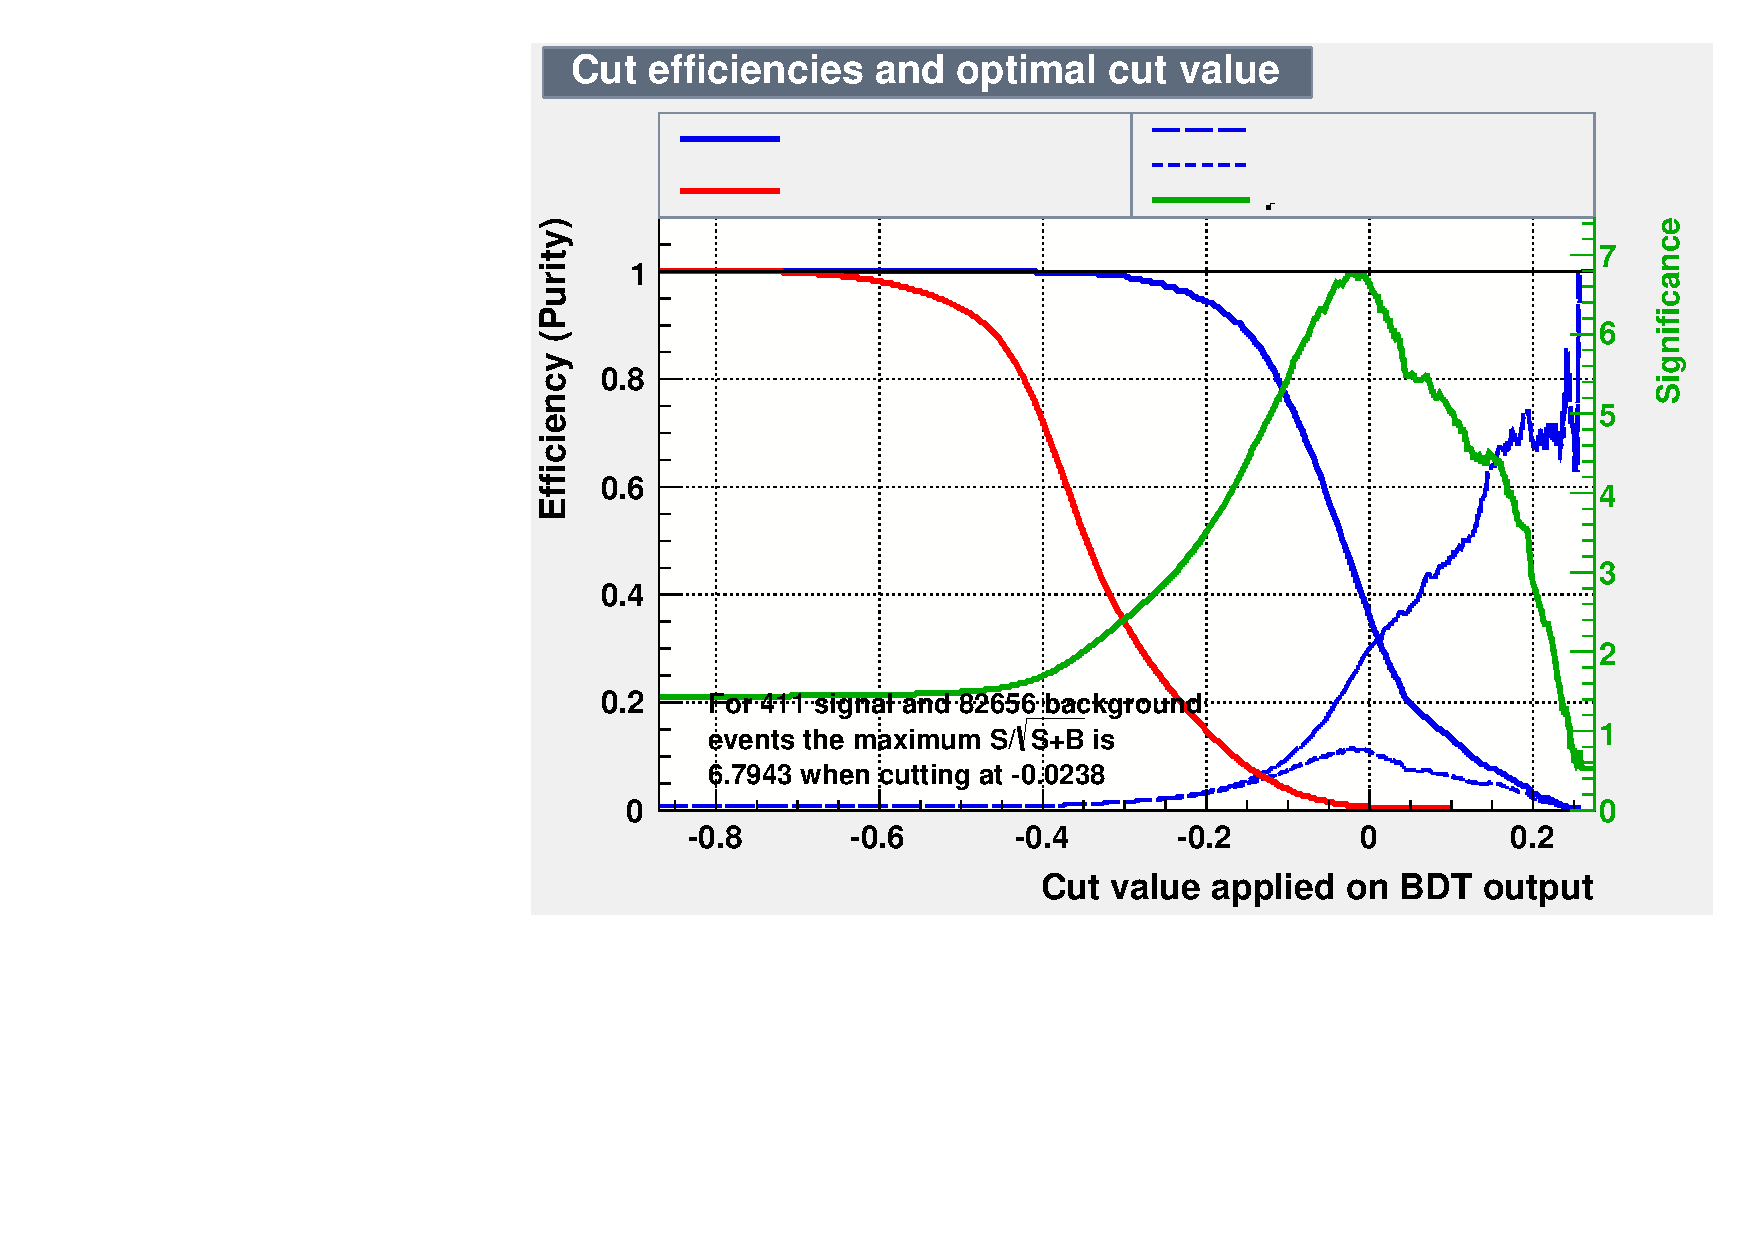
\includegraphics[width=0.6\linewidth]{{images/cutefficiences_1000trees2}.pdf}
  \caption{\scriptsize{The green line represents the statistical significance $\frac{S}{\sqrt{S+B}}$ where as it can be
  seen it reaches the greatest value at -0.0238. The cut is also known as descision boundary and defines the
  critical region.}}
  
 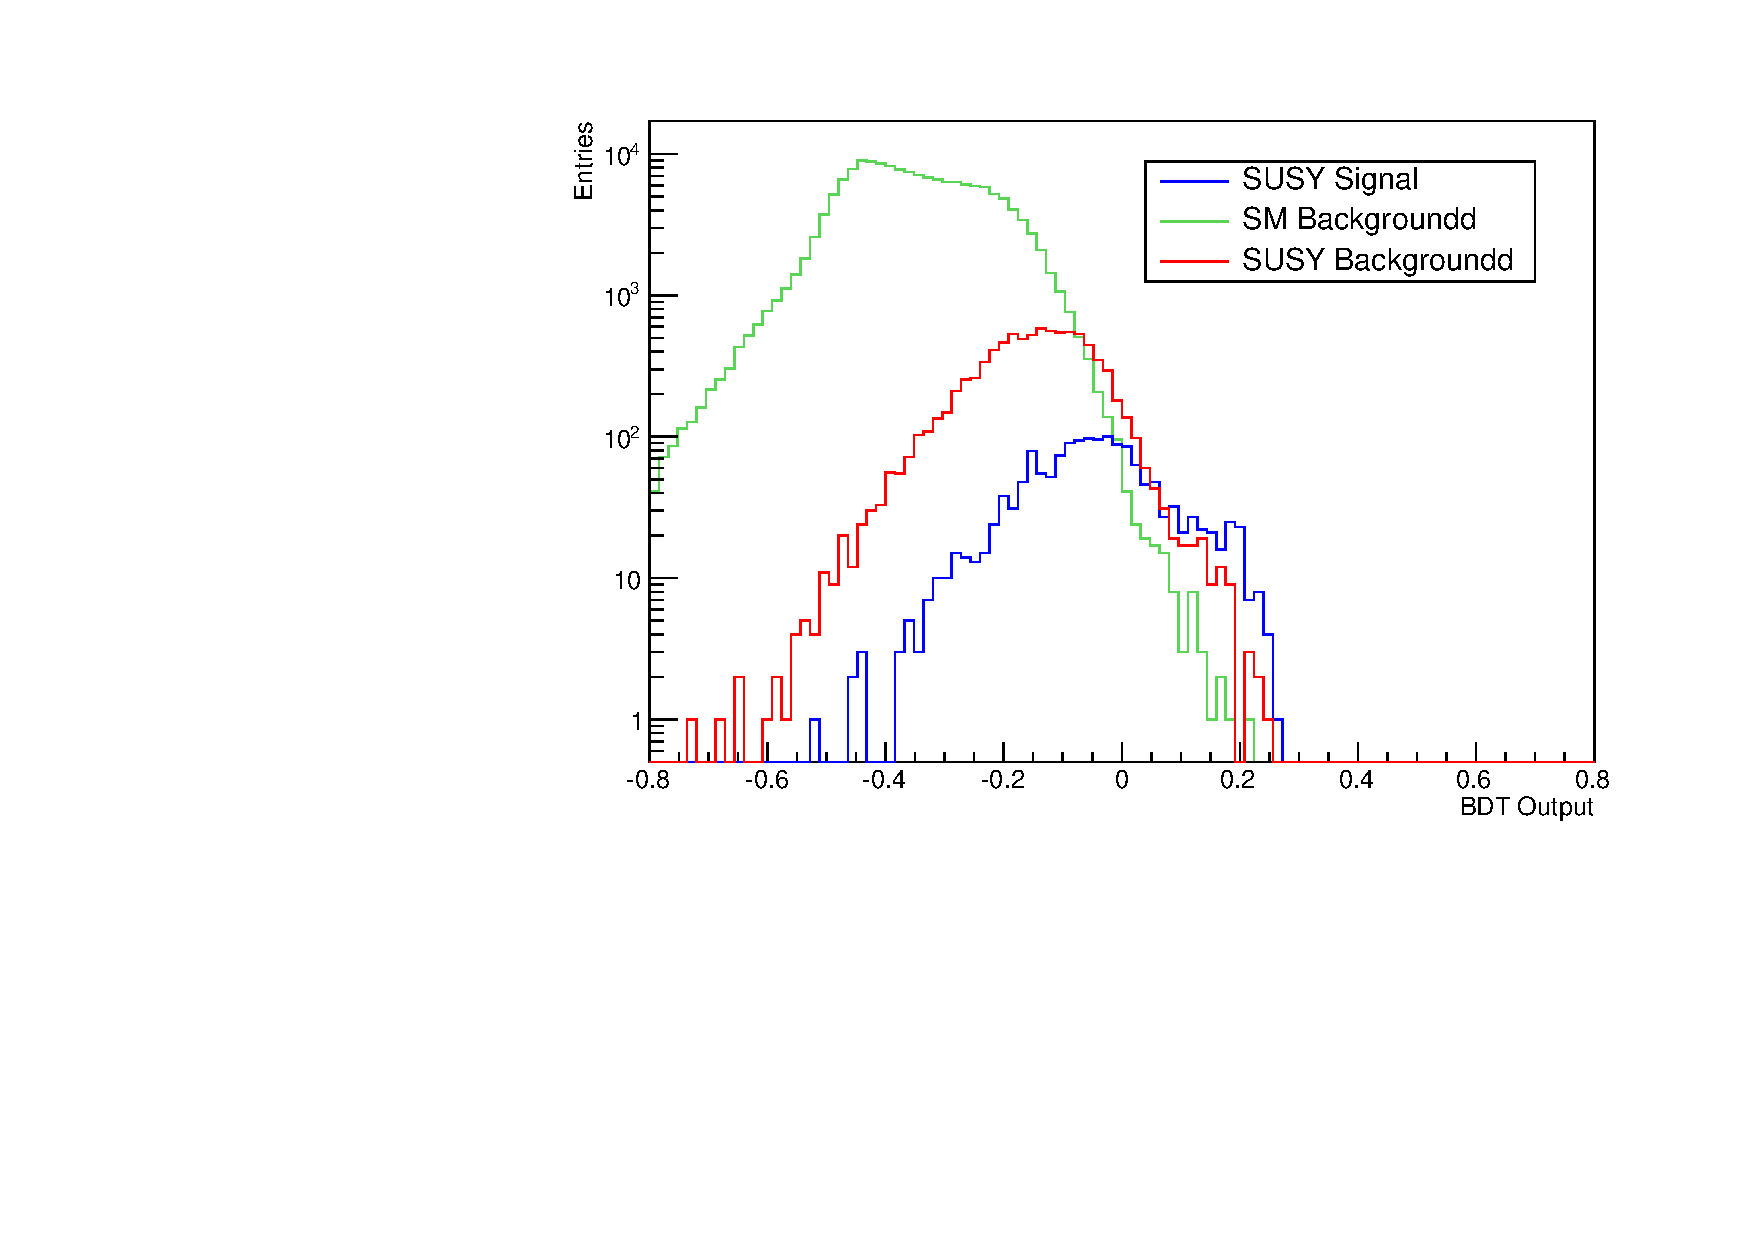
\includegraphics[width=0.6\linewidth]{{images/BDT_output_intlum3000}.pdf}
  \caption{\scriptsize{The BDT output for the signal and the two backgrounds. The y axis has a log scale.}}
\end{figure}

\newpage

After the training phase, the TMVA yields which variables where the most important in the classification
procedure where (ordered from the most significant):

\begin{enumerate}
 \item $\theta_{miss}$
 \item missing $p_{T}$ 
 \item $\Delta \phi$
 \item $cos\theta_{top}$
\end{enumerate}

The above histograms show the aforementioned variables as they were given for training and testing.


\begin{figure}
\begin{minipage}[c]{0.5\linewidth}
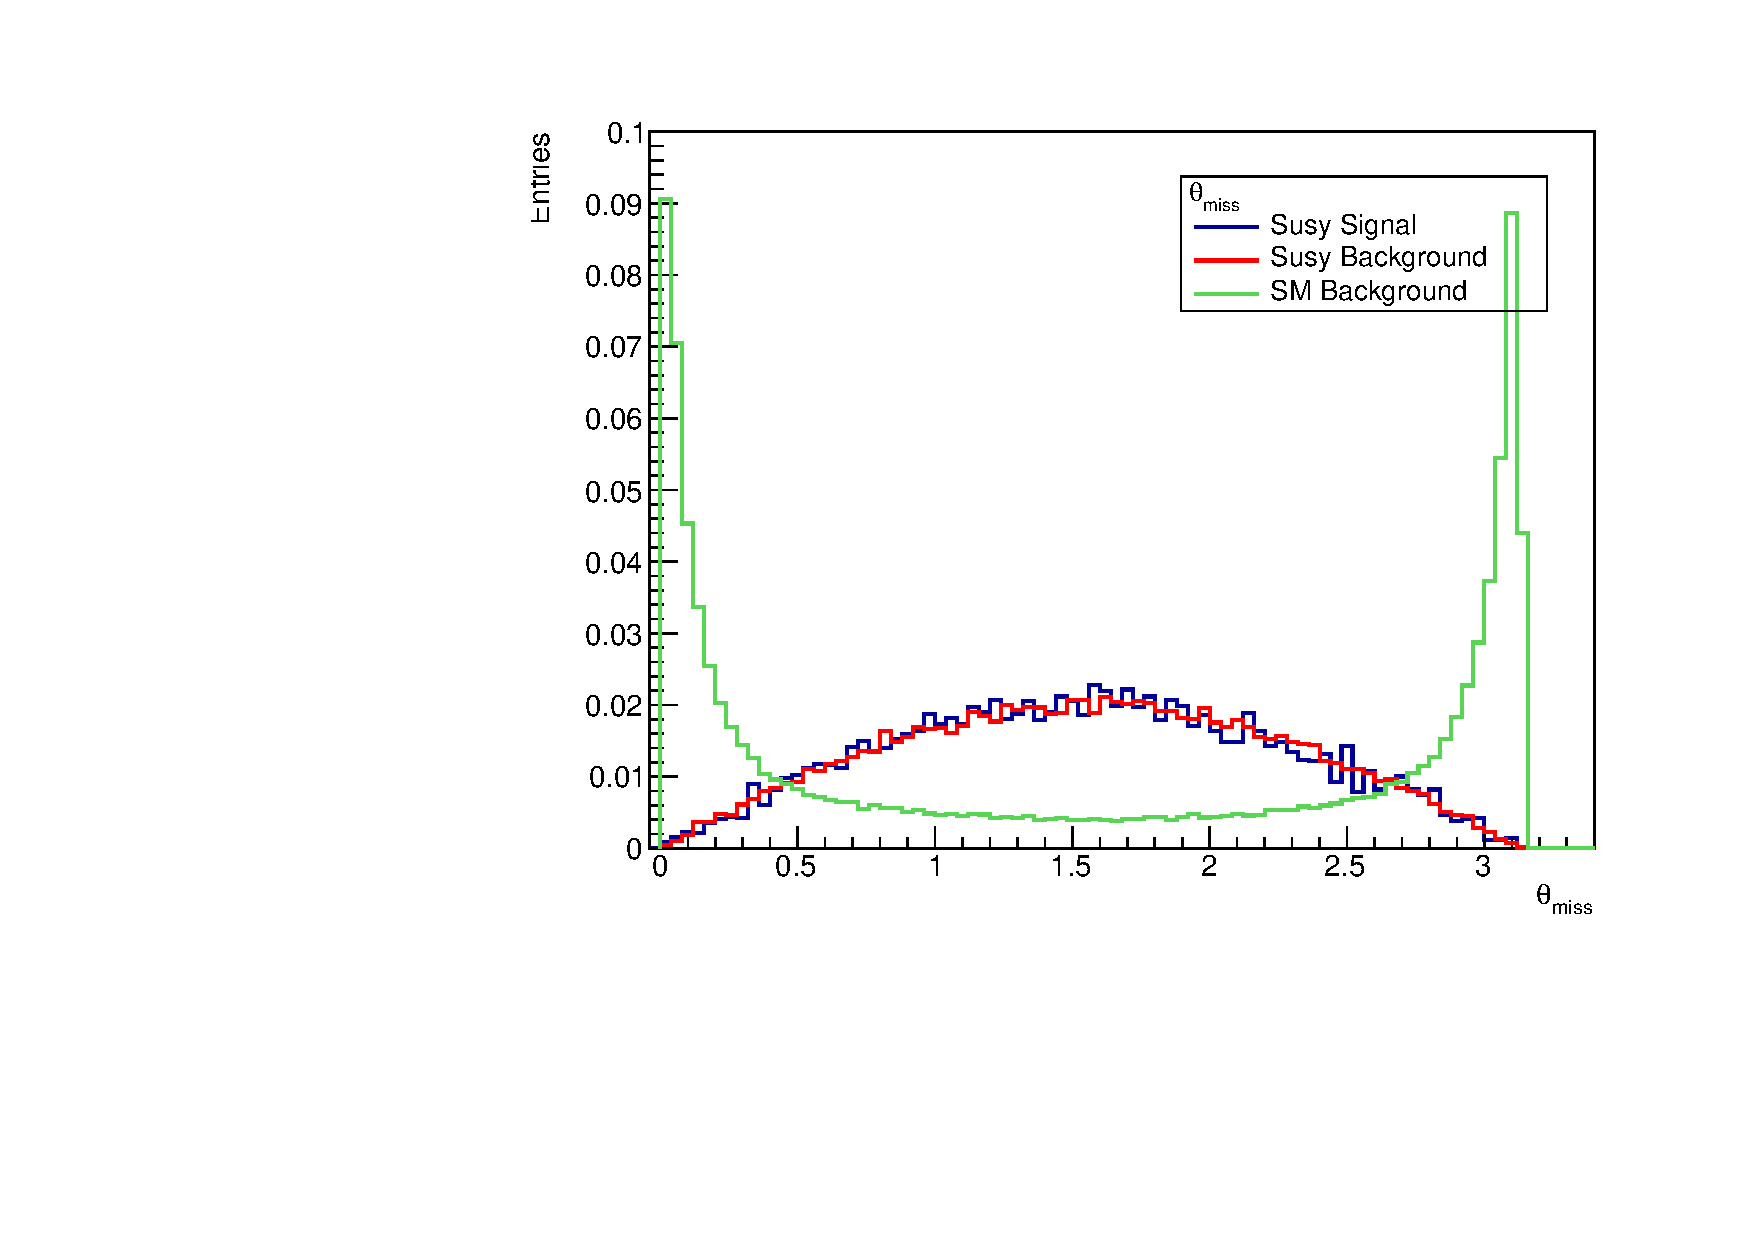
\includegraphics[width=\linewidth]{{images/thetamiss_report}.pdf}
\caption{\scriptsize{Polar angle of the missing momentum of the jets}}
\end{minipage}
\hfill
\begin{minipage}[c]{0.5\linewidth}
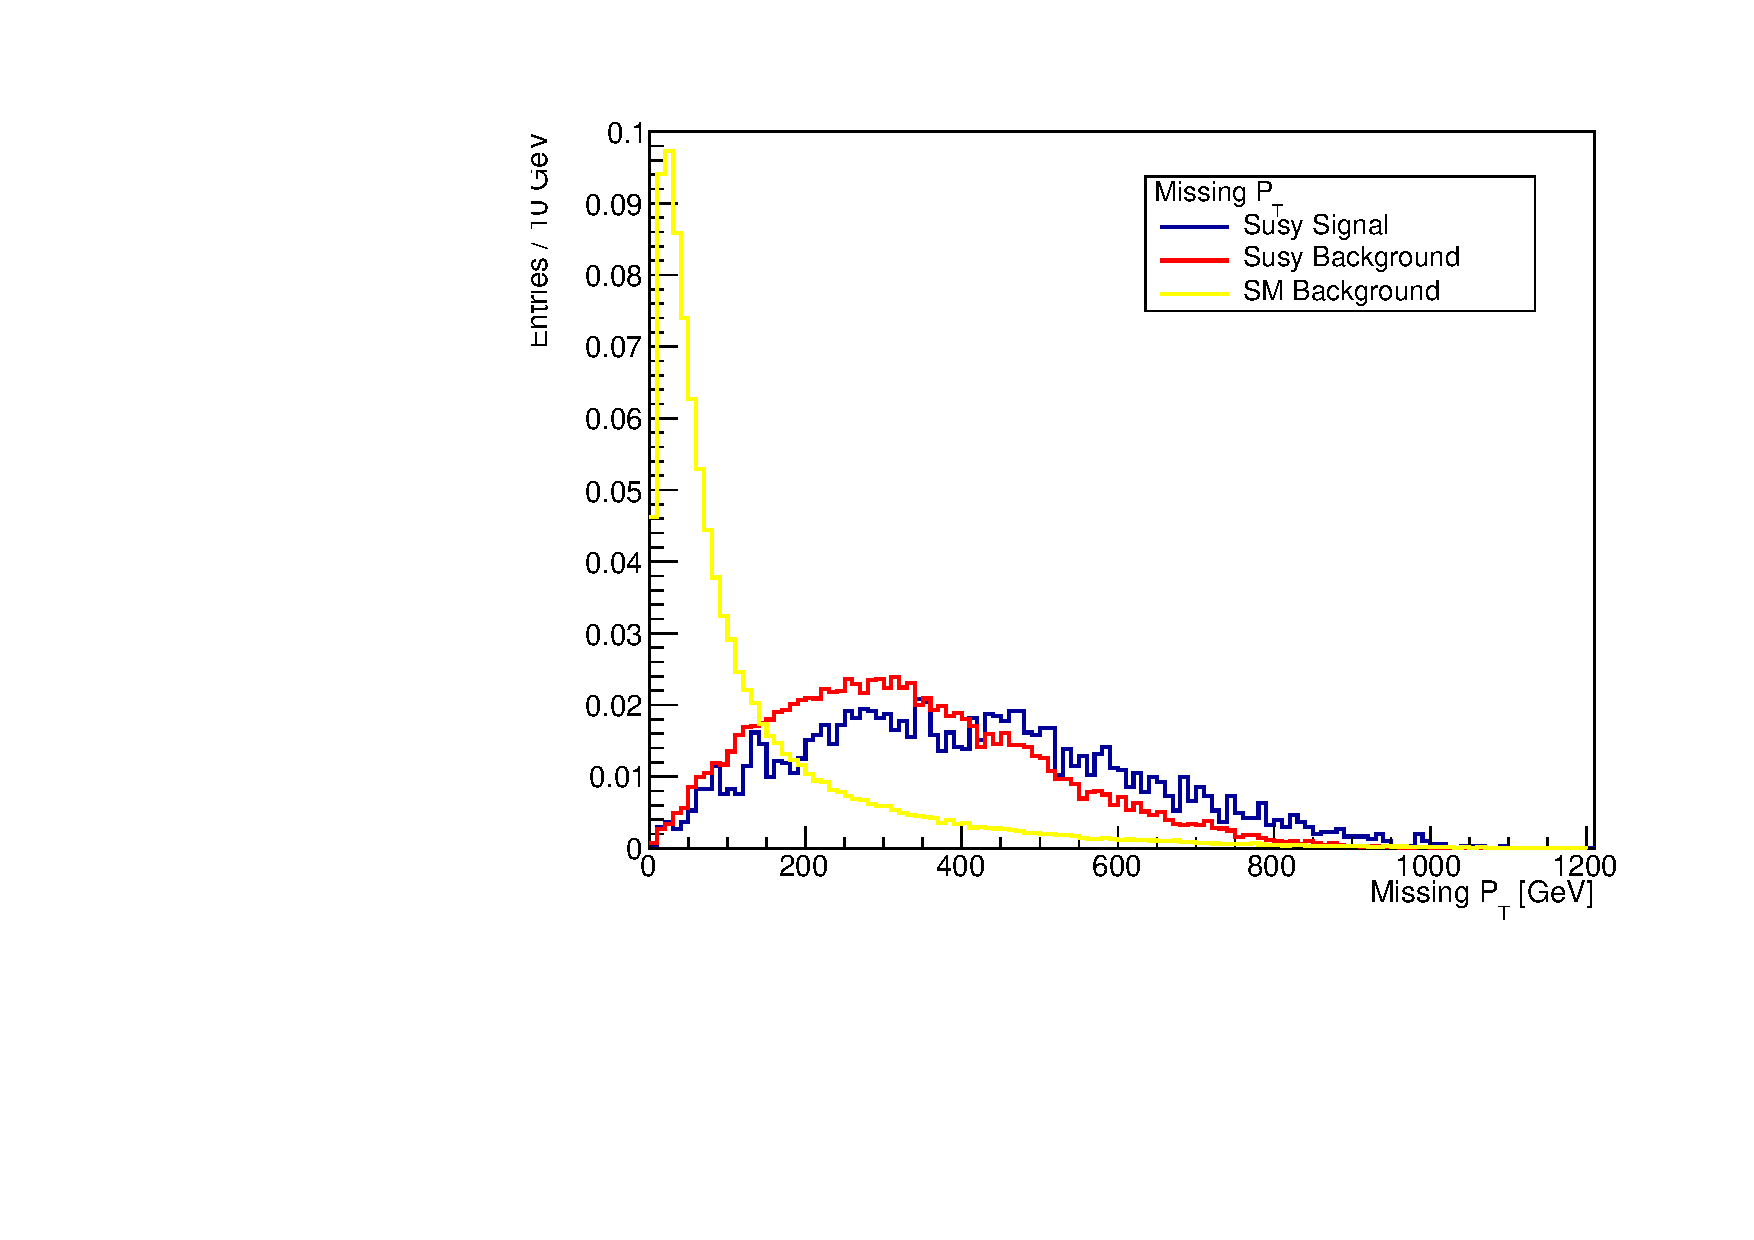
\includegraphics[width=\linewidth]{{images/missingptpfo_report}.pdf}
\caption{\scriptsize{Missing transverse momentum}}
\end{minipage}
\end{figure}

\begin{figure}
\begin{minipage}[c]{0.5\linewidth}
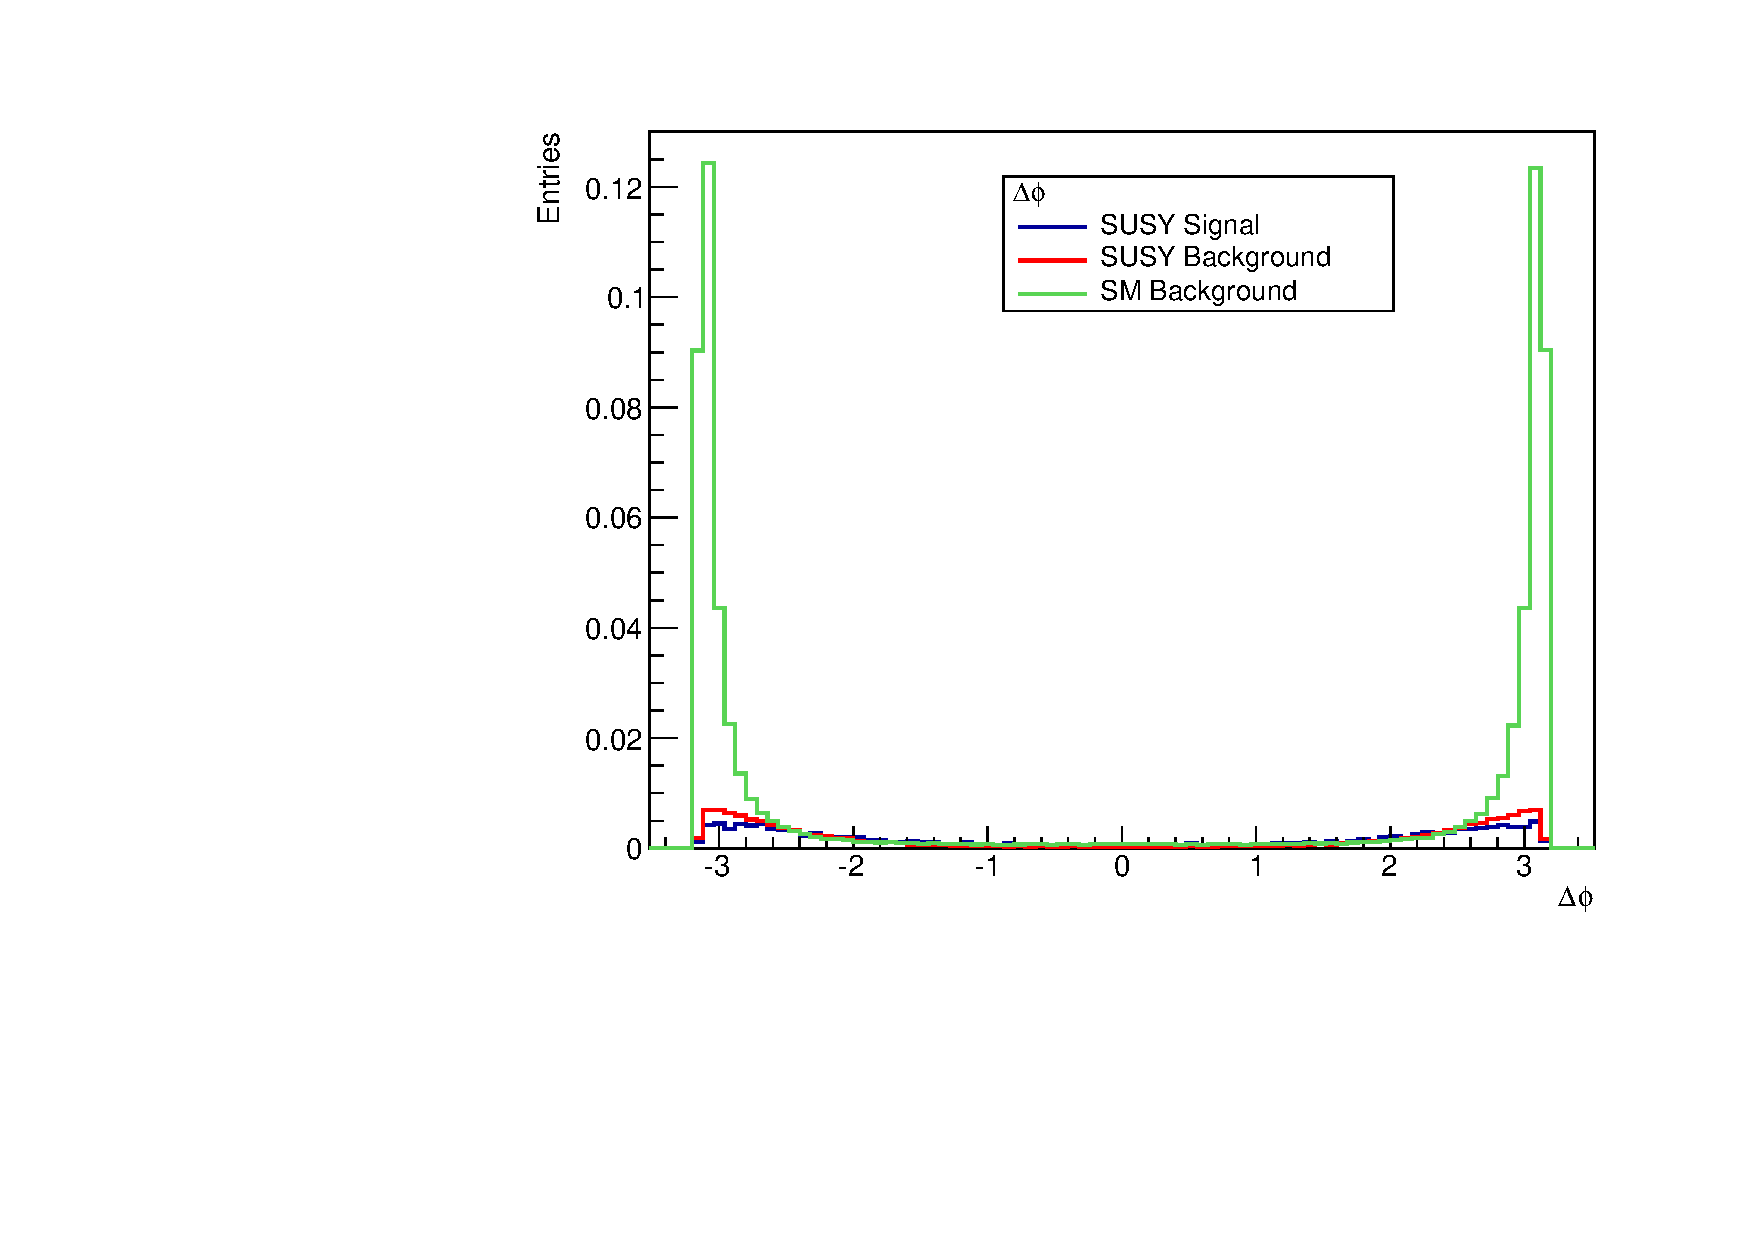
\includegraphics[width=\linewidth]{{images/deltaphi_report}.pdf}
\caption{\scriptsize{The angle between the reconstructed tops}}
\end{minipage}
\hfill
\begin{minipage}[c]{0.5\linewidth}
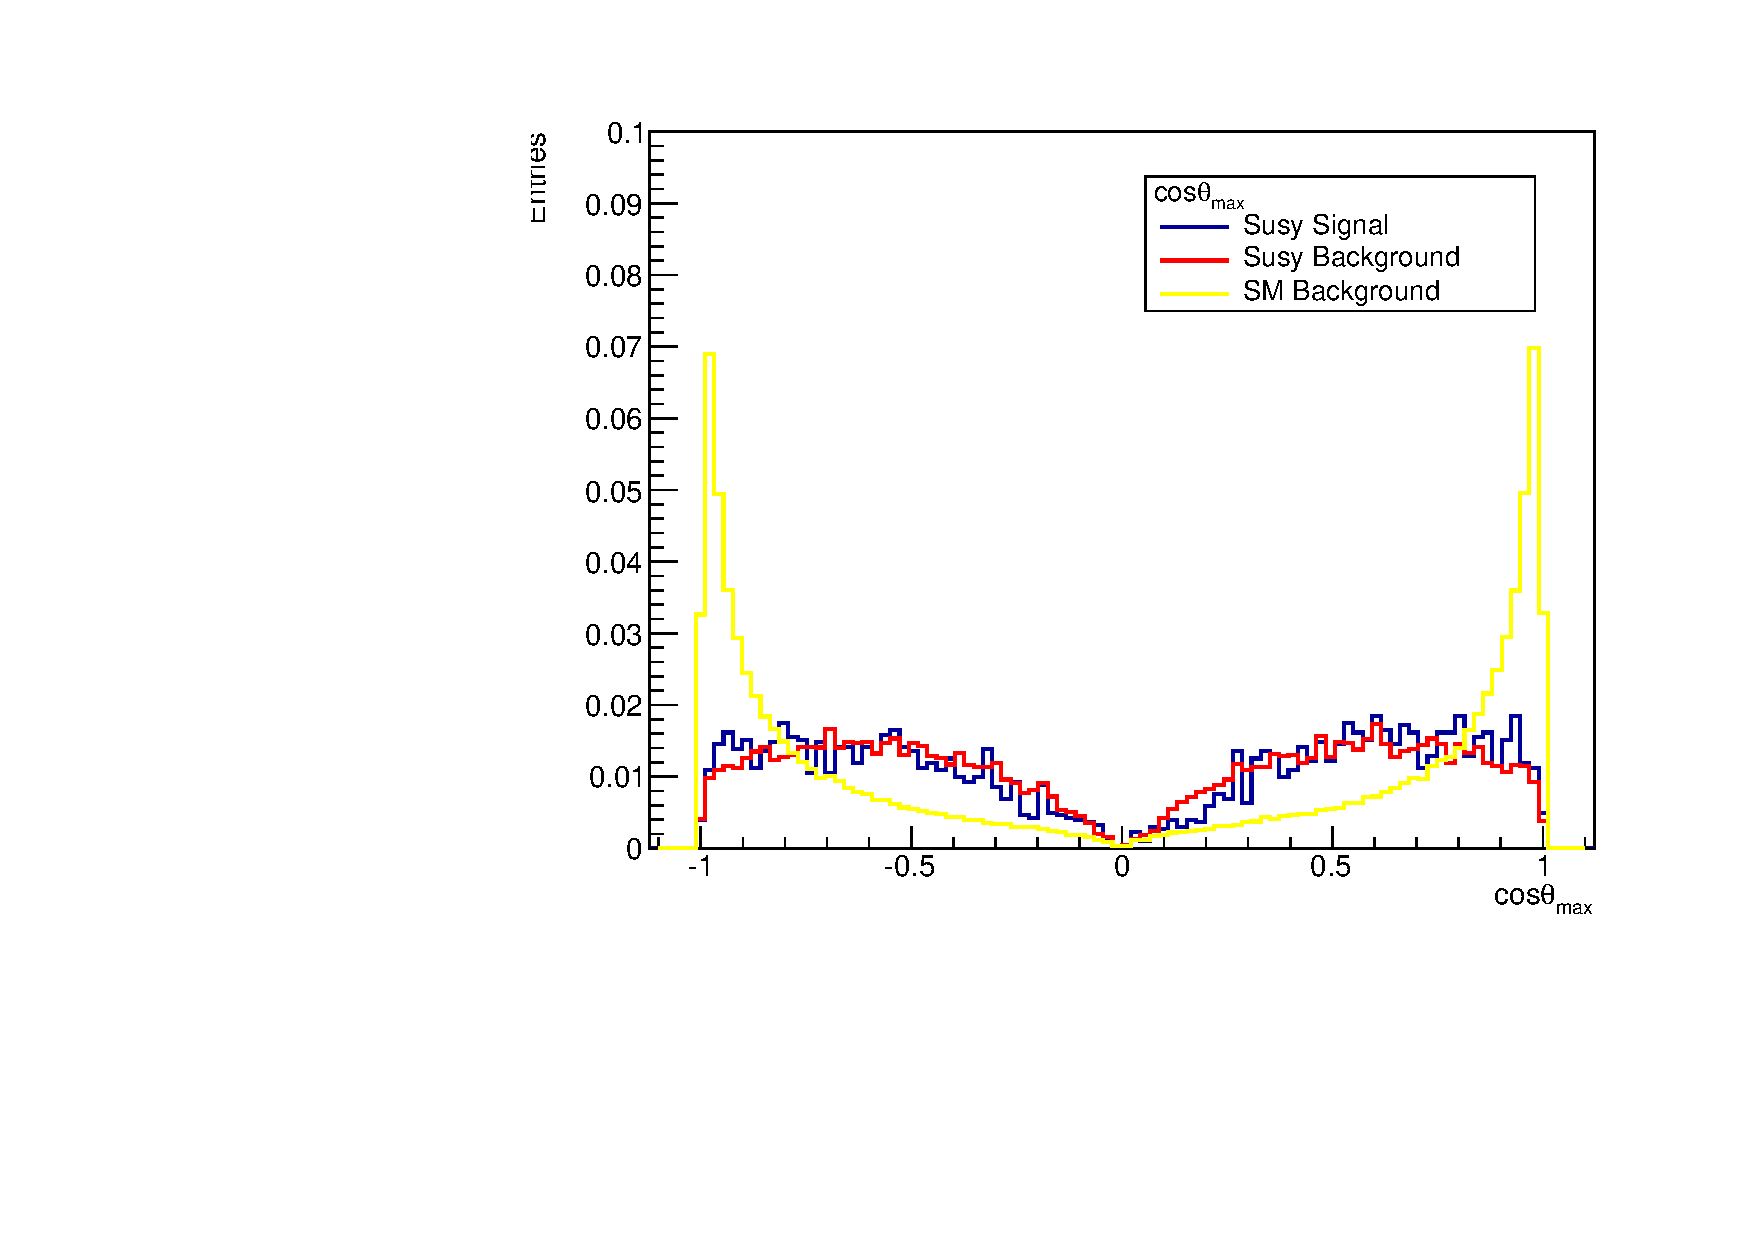
\includegraphics[width=\linewidth]{{images/costhetatopmax}.pdf}
\caption{\scriptsize{cos$\theta_{top}$}}
\end{minipage}
\end{figure}

\newpage

\subsubsection{Energy Spectrum of the Reconstructed Top quark}

In the histogram below the energy spectrum of the top quark can be seen for the signal events.
This variable was not given to the TMVA for training and testing. 
It is clear that the maximum value of the energy is 1200 Tev something that explains why this was also set  
as a preselection cut. 

\begin{figure}[ht!]
  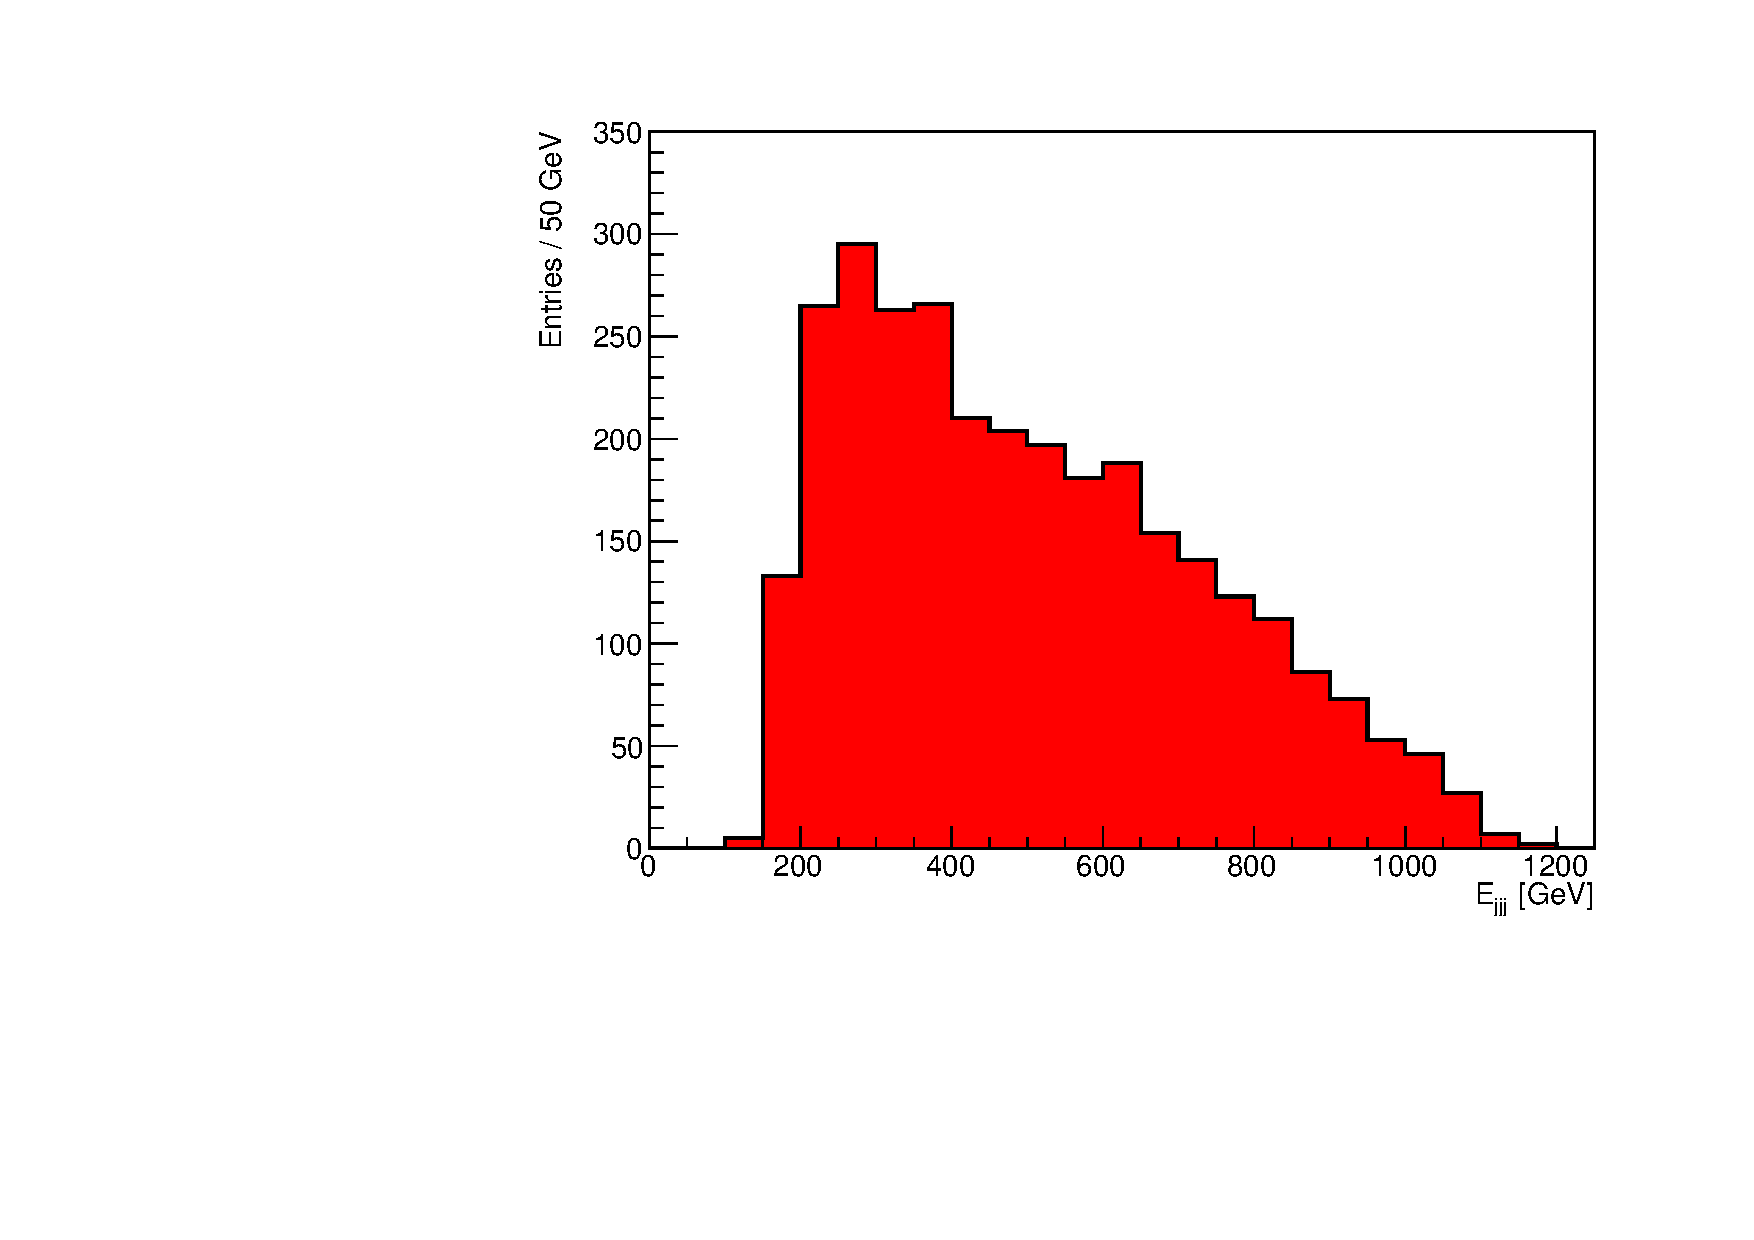
\includegraphics[width=0.7\linewidth]{{images/E_jjj}.pdf}
  \caption{\scriptsize{The energy of the top quark. For higher energies there are less entries per bin, something that
  is connected with the effect of Beamsstrahlung radiadion that is manifested mainly in higher energies.}}
\end{figure}


\begin{figure}[ht!]
  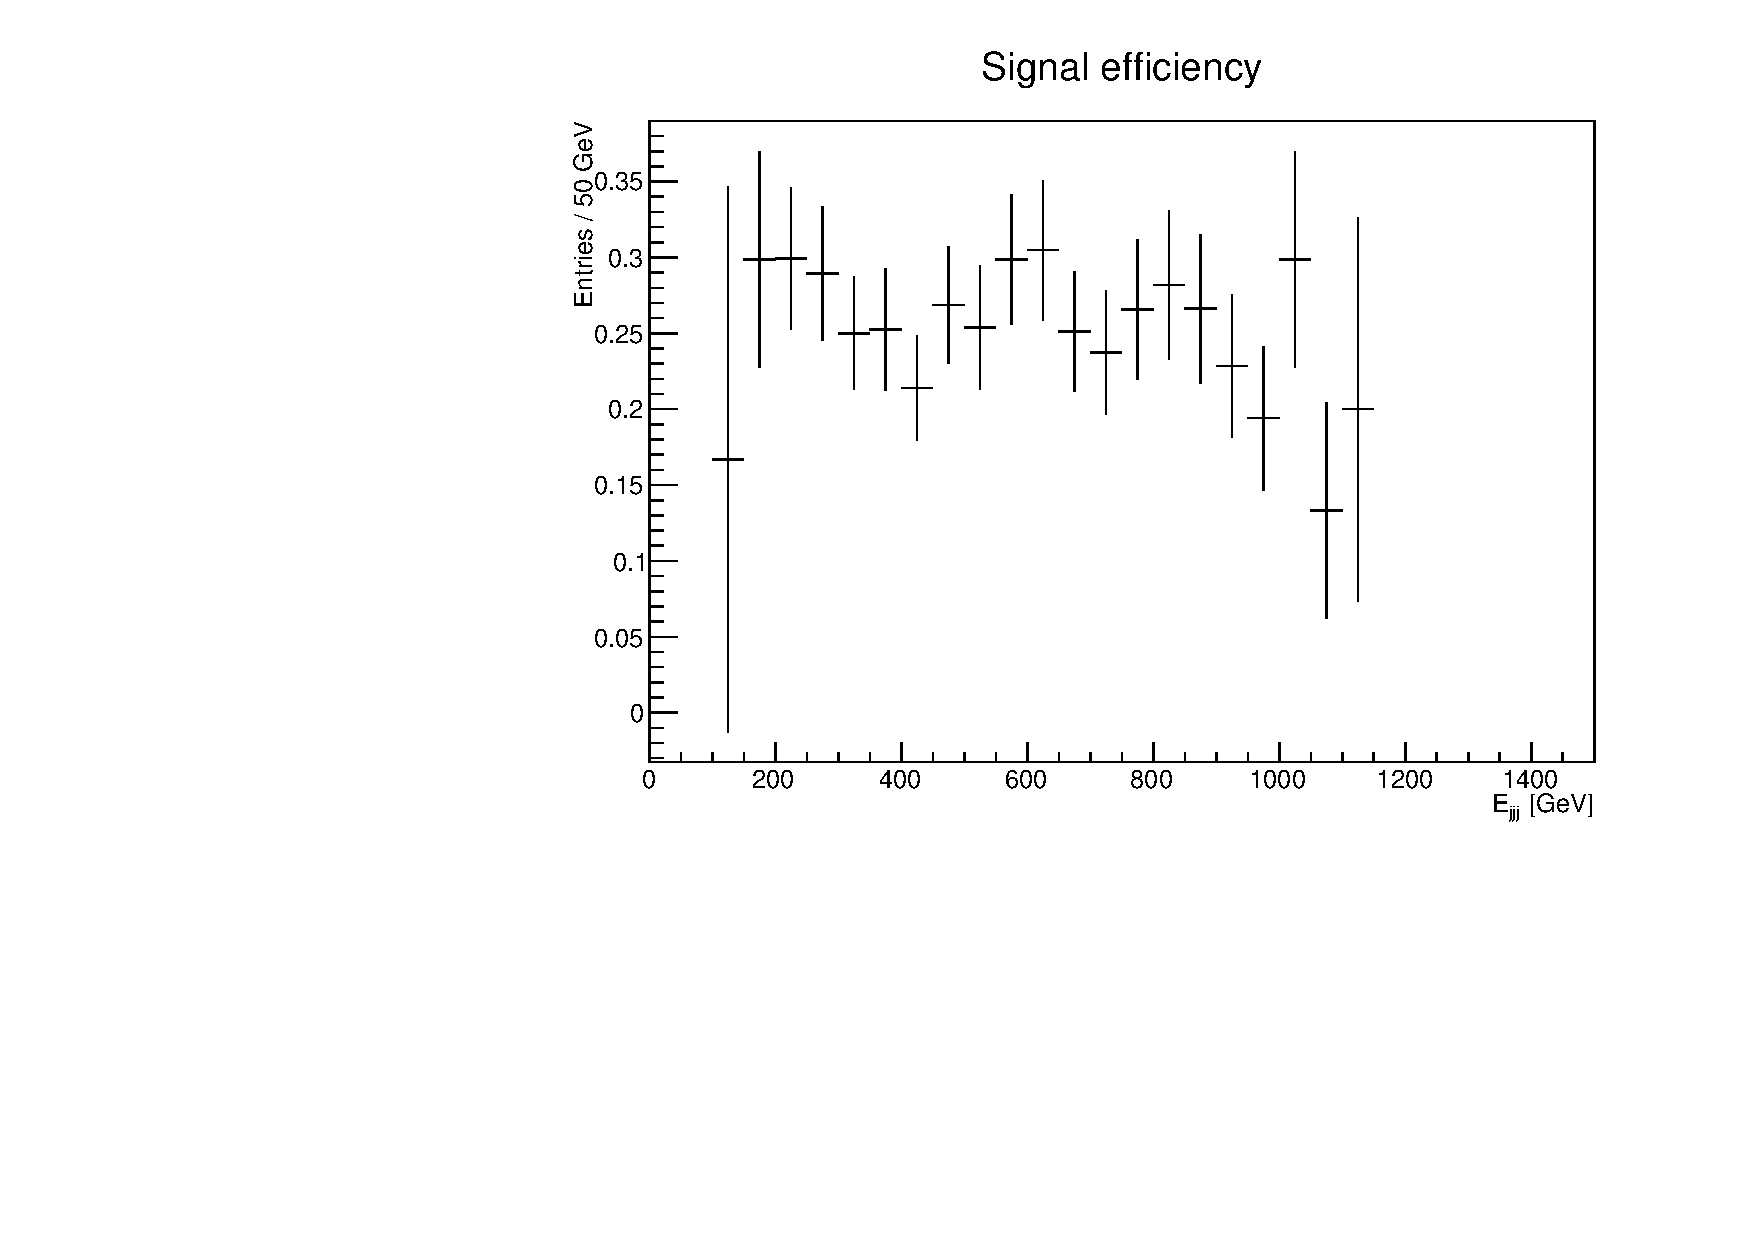
\includegraphics[width=0.7\linewidth]{{images/ratio_plot_witherrors}.pdf}
  \caption{\scriptsize{}}
\end{figure}

In the above histogram it can be seen the signal efficiency (with errors) as with respect to the energy of the three jets
$E_{jjj}$. It is defined to be the ratio of the number of events that passed the $cut_{BDT}$ over the total
number of the signal events.


For completenes, the above diagrams depict the SM background efficiency and the SUSY background efficiency.

\begin{figure}
\begin{minipage}[c]{0.6\linewidth}
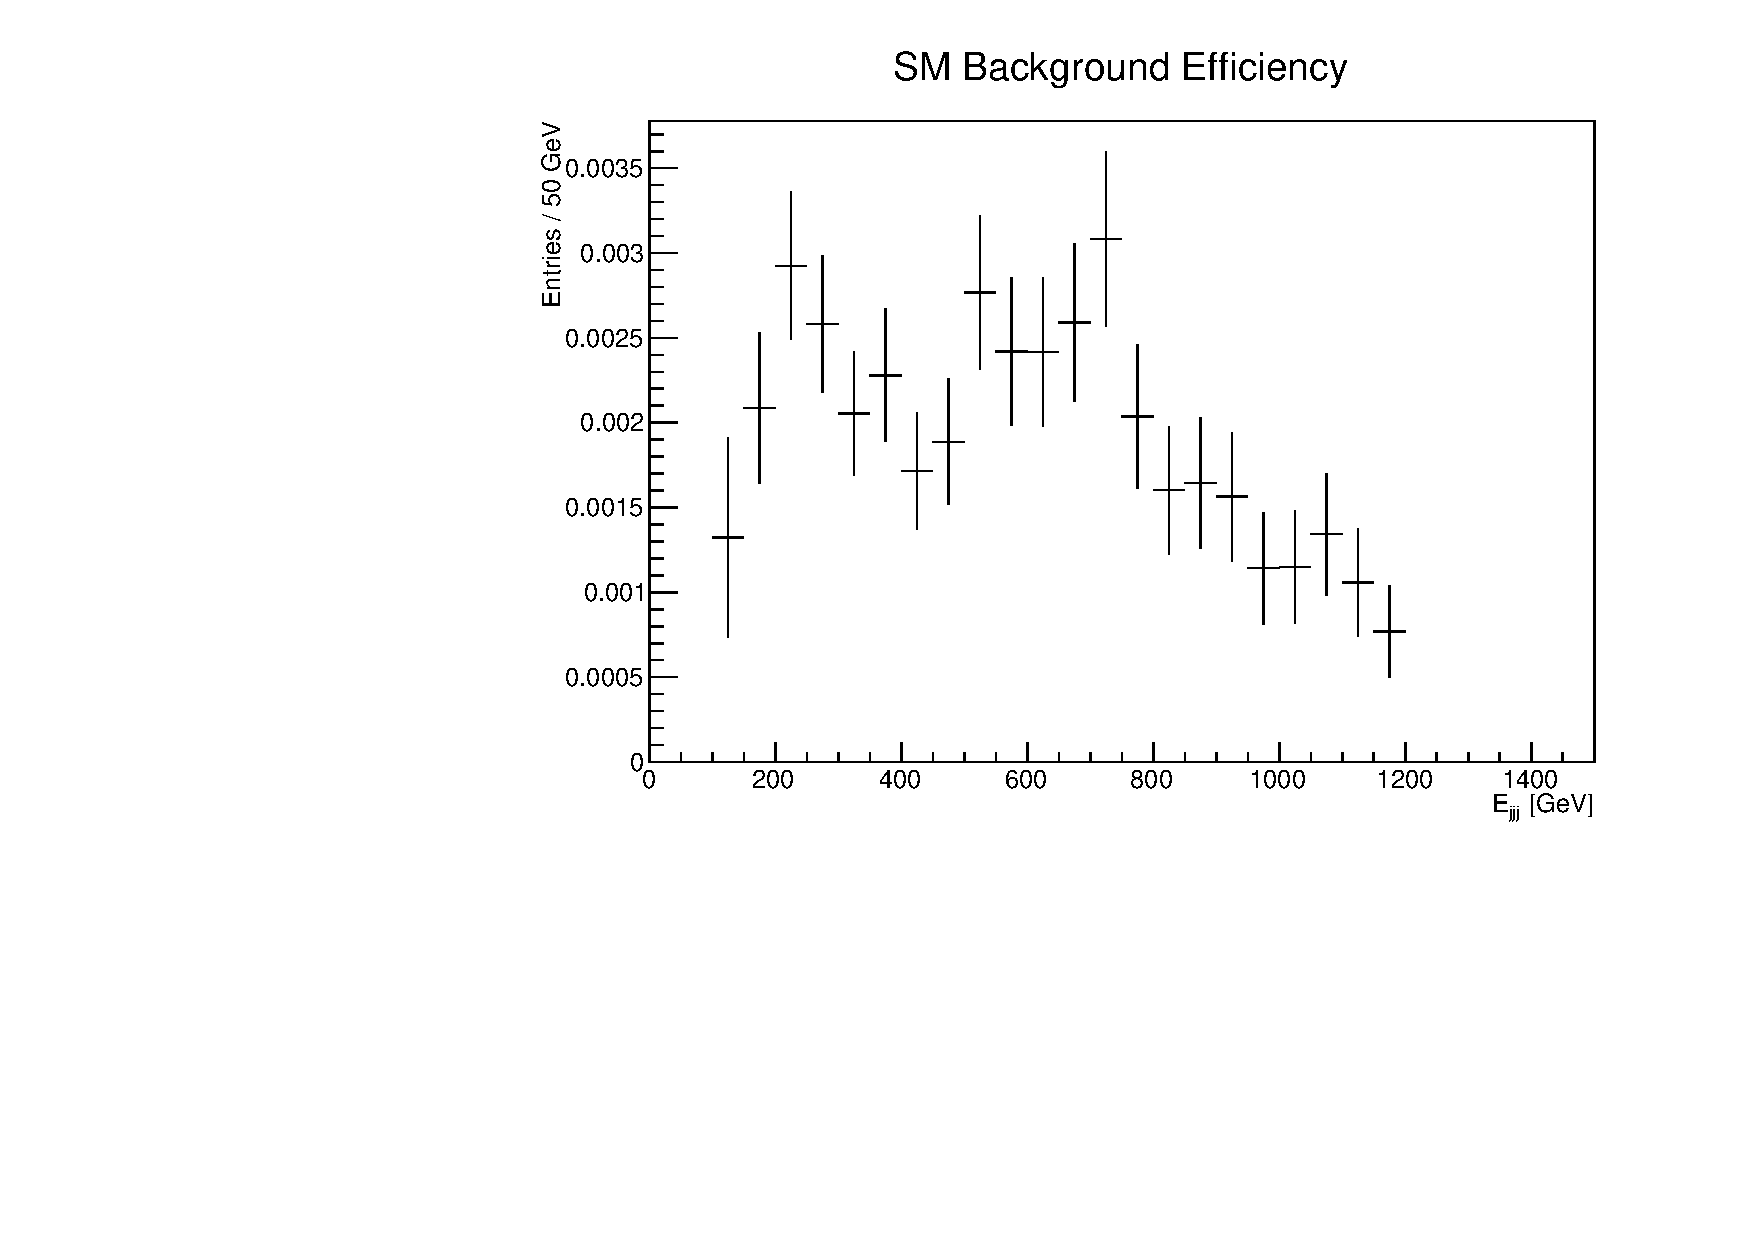
\includegraphics[width=\linewidth]{{images/ratio_plot_SMbackground_witherrors}.pdf}
\caption{\scriptsize{The Standard Model Background Efficiency}}
\end{minipage}
\hfill
\begin{minipage}[c]{0.6\linewidth}
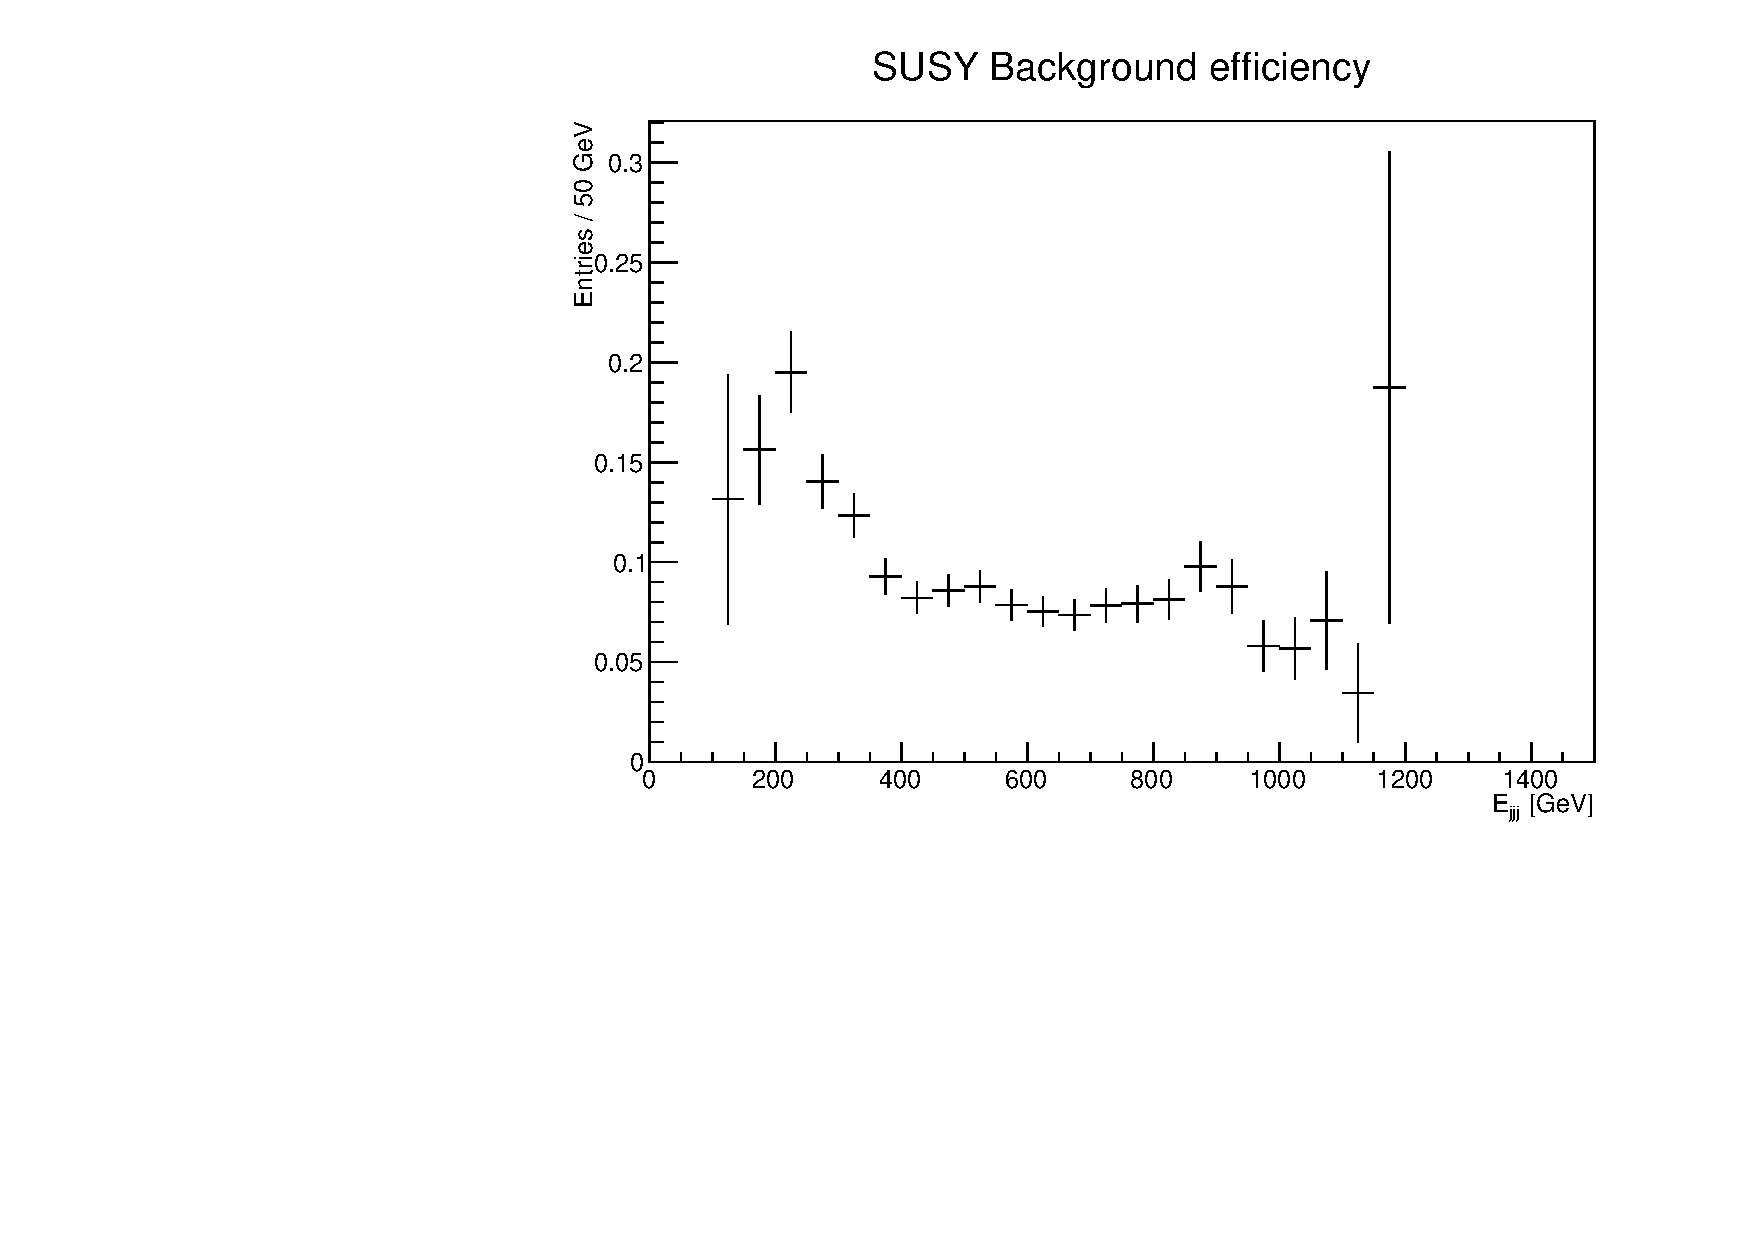
\includegraphics[width=\linewidth]{{images/ratio_plot_susybg_witherrors}.pdf}
\caption{\scriptsize{The SUSY Background Efficiency}}
\end{minipage}
\end{figure}

\newpage

\subsubsection{Effectiveness of BDT's}

In the following graphs we can see the number of events of the signal and the two backgrounds with respect
of the $E_{jjj}$ before and after the $cut_{BDT}$. As it can be seen, the Standard Model Background as well as
the SUSY Background have reduced significantly.


\begin{figure}[ht!]
  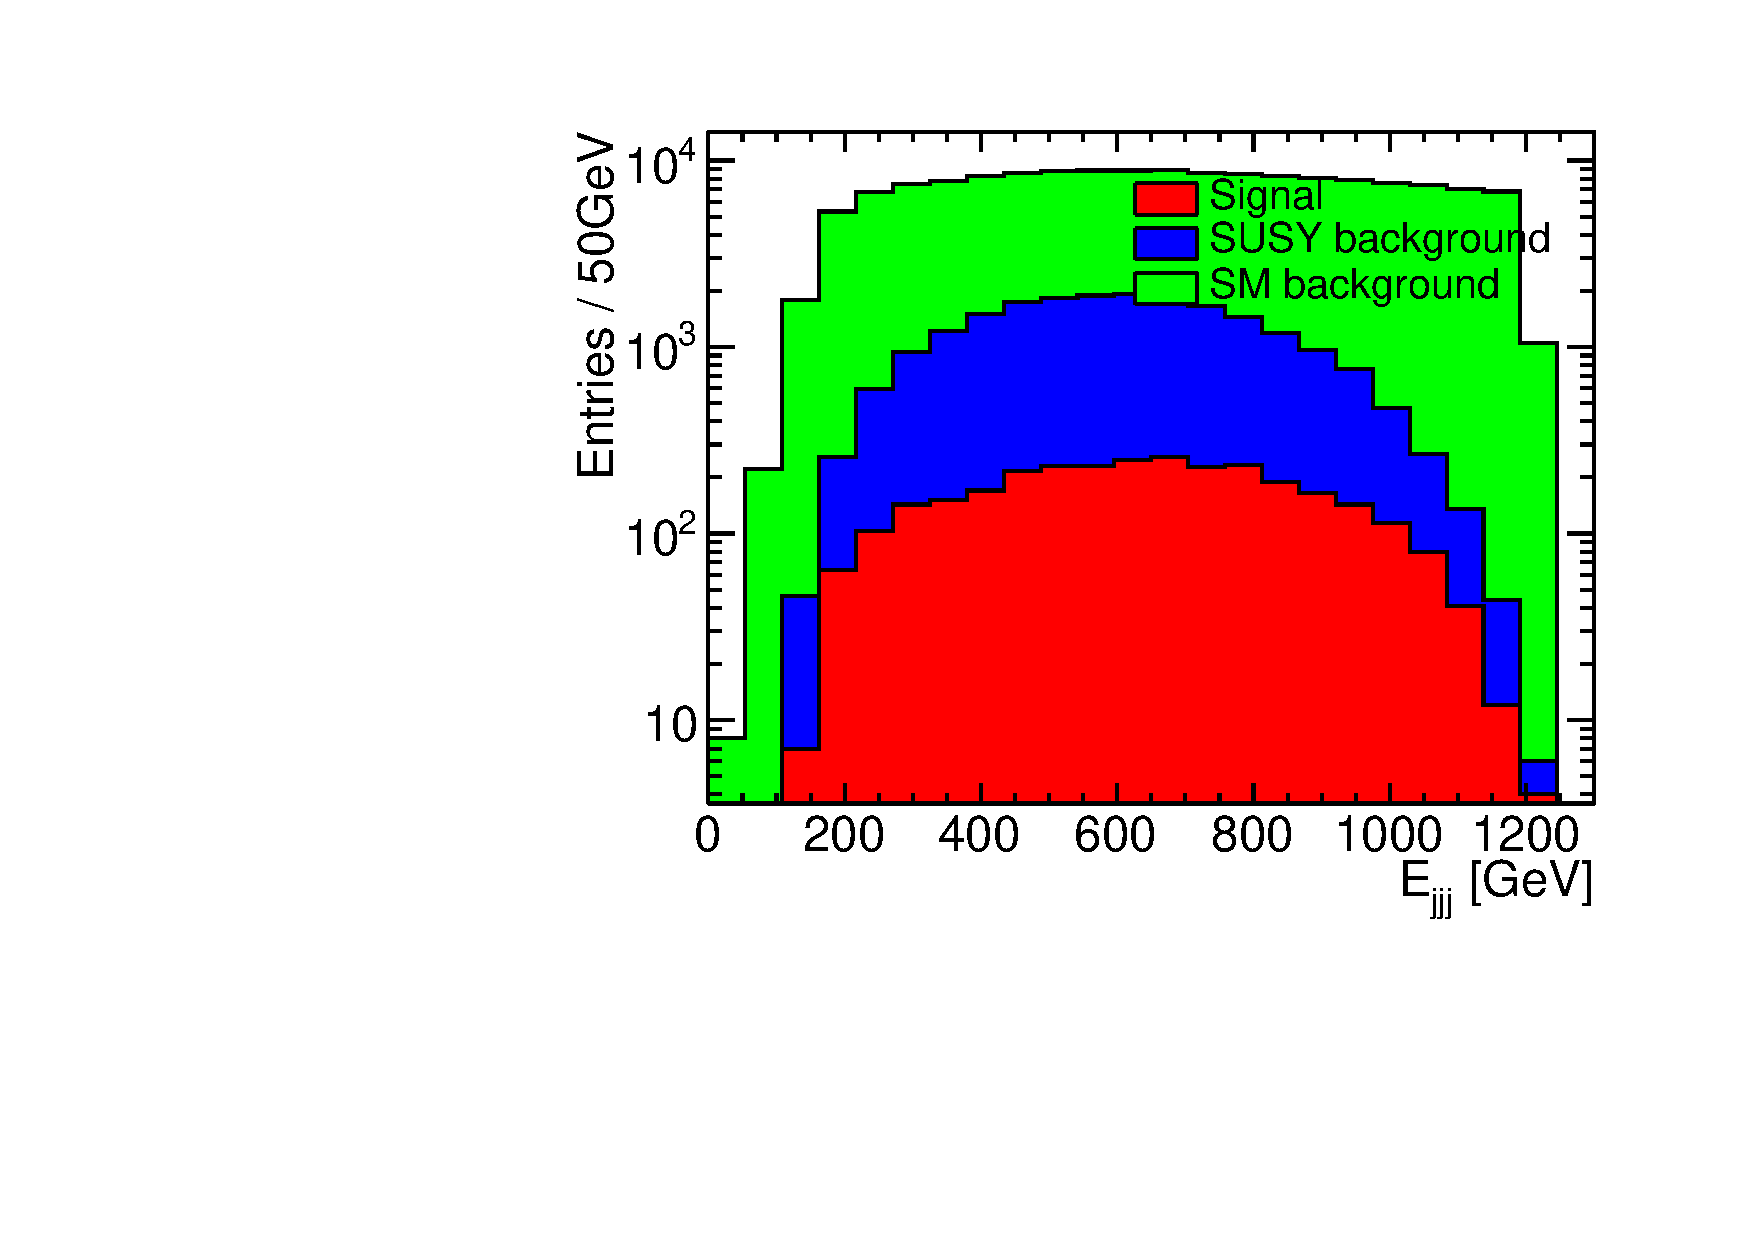
\includegraphics[width=0.7\linewidth]{{images/prebdtcut}.pdf}
  \caption{\scriptsize{Signal, SM background and SUSY background before the TMVA application. It is a 
  stacked histogram with log y axis.}}
\end{figure}

\begin{figure}[ht!]
  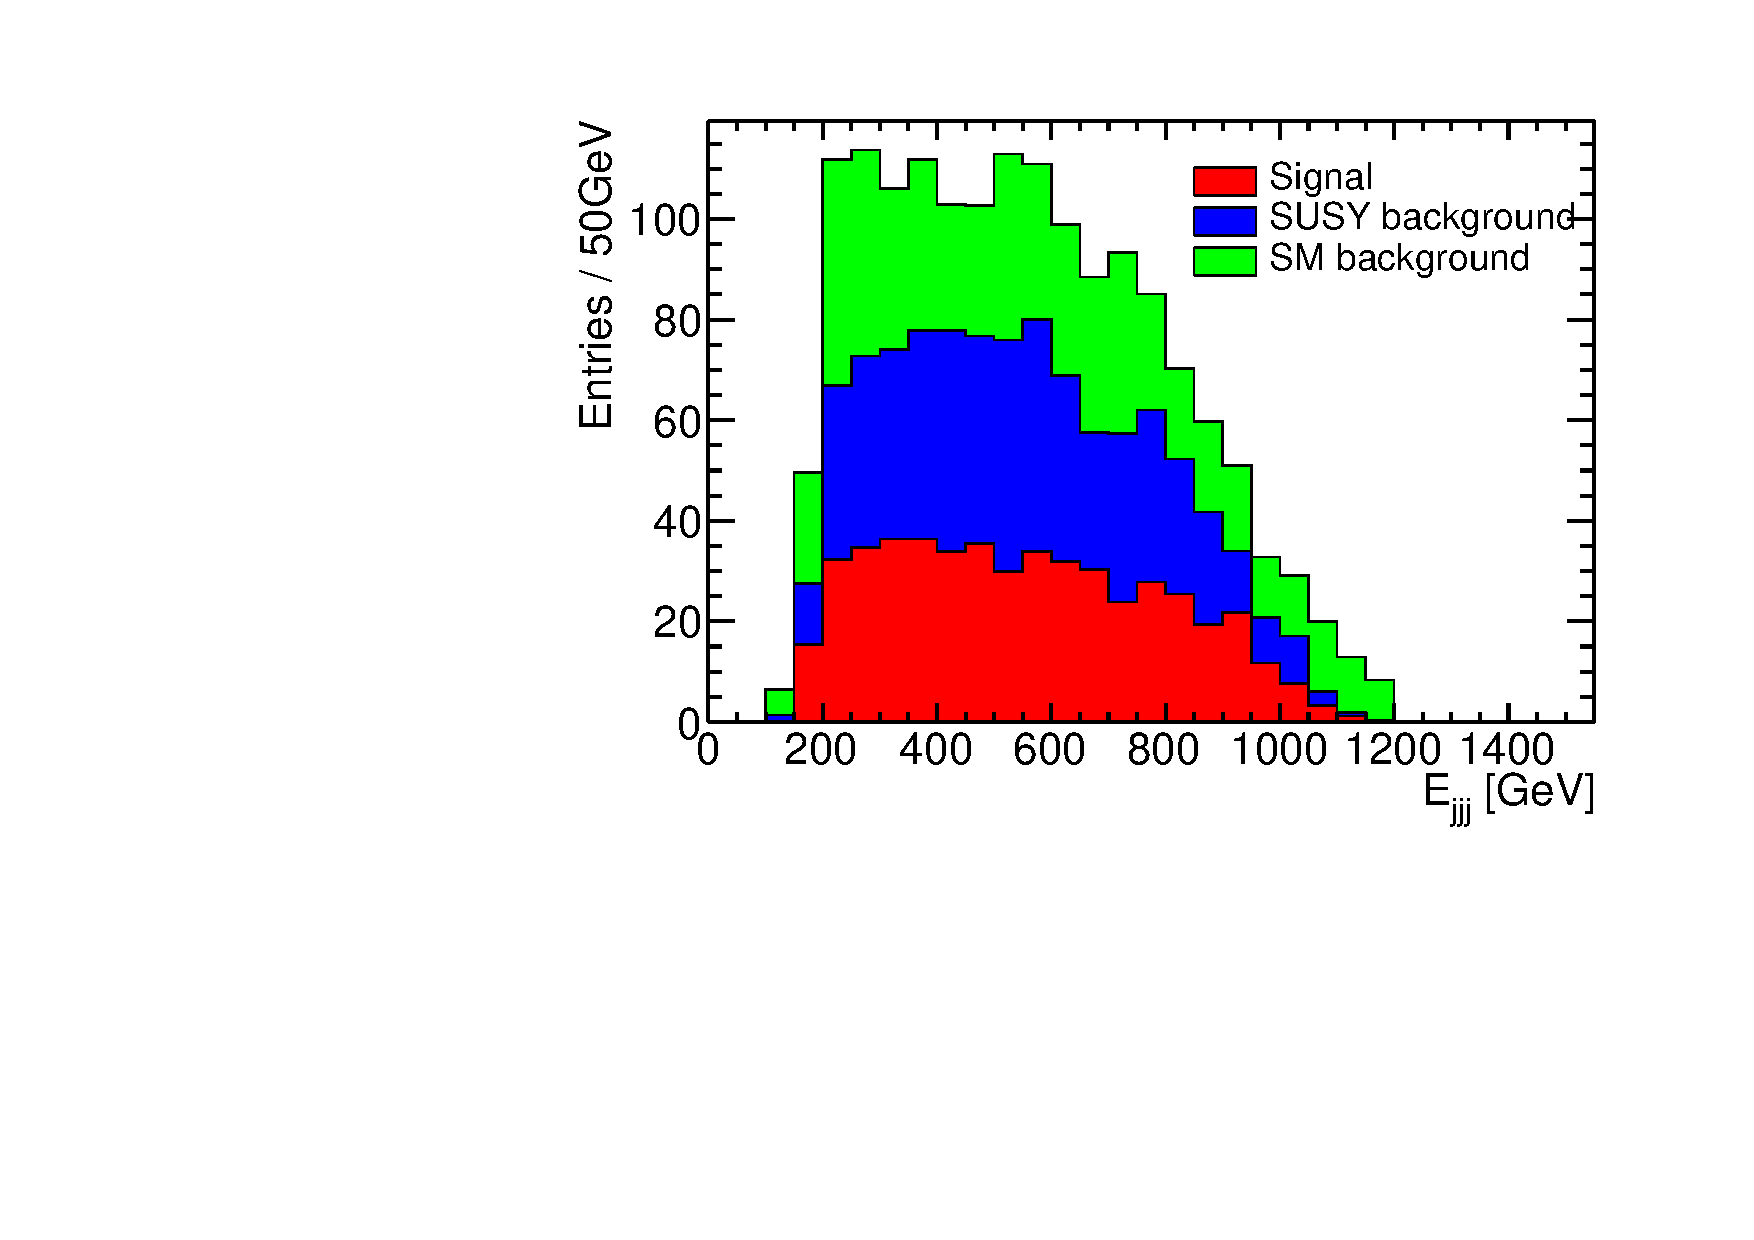
\includegraphics[width=0.7\linewidth]{{images/postbdtcut_intlumi3000}.pdf}
  \caption{\scriptsize{Signal, SM background and SUSY background after the TMVA application, again stacked.}}
\end{figure}

\newpage

The following table summarises the number of events that passed the preselection cuts, before and after the 
TMVA cut.

\begin{table}
\centering % used for centering table
\begin{tabular}{||c | c | c | c||} % centered columns (4 columns)
\hline %inserts double horizontal lines
       BDT      &Before TMVA ($N_{events}$)  & After TMVA ($N_{events}$) & $\%$  \\ \hline % inserts single horizontal line
Signal           & 3005     &  493       & 16 \\
SUSY background  & 17628    &  558       & 3.1 \\
SM background    & 113494   &  528       &  0.4 \\  
\hline
 %inserts single line
\end{tabular}
\label{table:nonlin} % is used to refer this table in the text
\end{table}

\subsubsection{Mass Calculation Results}

For the calculation of the top squark mass I made use of the minimisation of the $\chi^{2}$ method. In this 
method we calculate the $\chi^{2}$ value for different masses of the top squark, and the minimum of the fitted
polynomial yields the mass.

Concretely, the formula for the calculation of the $\chi^{2}$ is:

\begin{equation}
 \chi^{2}=\sum_{i}^{}\frac{(n_{data,i}-n_{template,i})^{2}}{\sigma_{data,i}^{2}+\sigma_{template,i}^{2}}
\end{equation}

where $n_{data}$ are the number of events in the energy spectrum of the three jets after the TMVA (figure 4.12)
and $n_{template}$ are the number of events for each different template, while the sum runs over all the bins
of the histogram. A $\chi^{2}$ was calculated for each different template, summarised in the table below.


\hfill

\begin{table}[h]
\centering % used for centering table
\begin{tabular}{||c | c||} % centered columns (4 columns)
\hline \hline %inserts double horizontal lines
$M_{template}$ 		   & $\sigma$ (fb)   \\ \hline % inserts single horizontal line
$M_{nom}$ -200 GeV         &   2.8   \\
$M_{nom}$ -100 GeV         &   2.2   \\
$M_{nom}$ -50  GeV         &   1.9   \\  
$M_{nom}$        	   &  1.65   \\
$M_{nom}$ +50  GeV	   &   1.4   \\
$M_{nom}$ +100 GeV	   &   1.2   \\
$M_{nom}$ +200 GeV	   &   0.8   \\

\hline
 %inserts single line
\end{tabular}
\label{table:nonlin} % is used to refer this table in the text
\end{table}

The mass was found  to be $m_{\tilde{t}}$ = 839 GeV.


\newpage

\begin{figure}[ht!]
\centering
  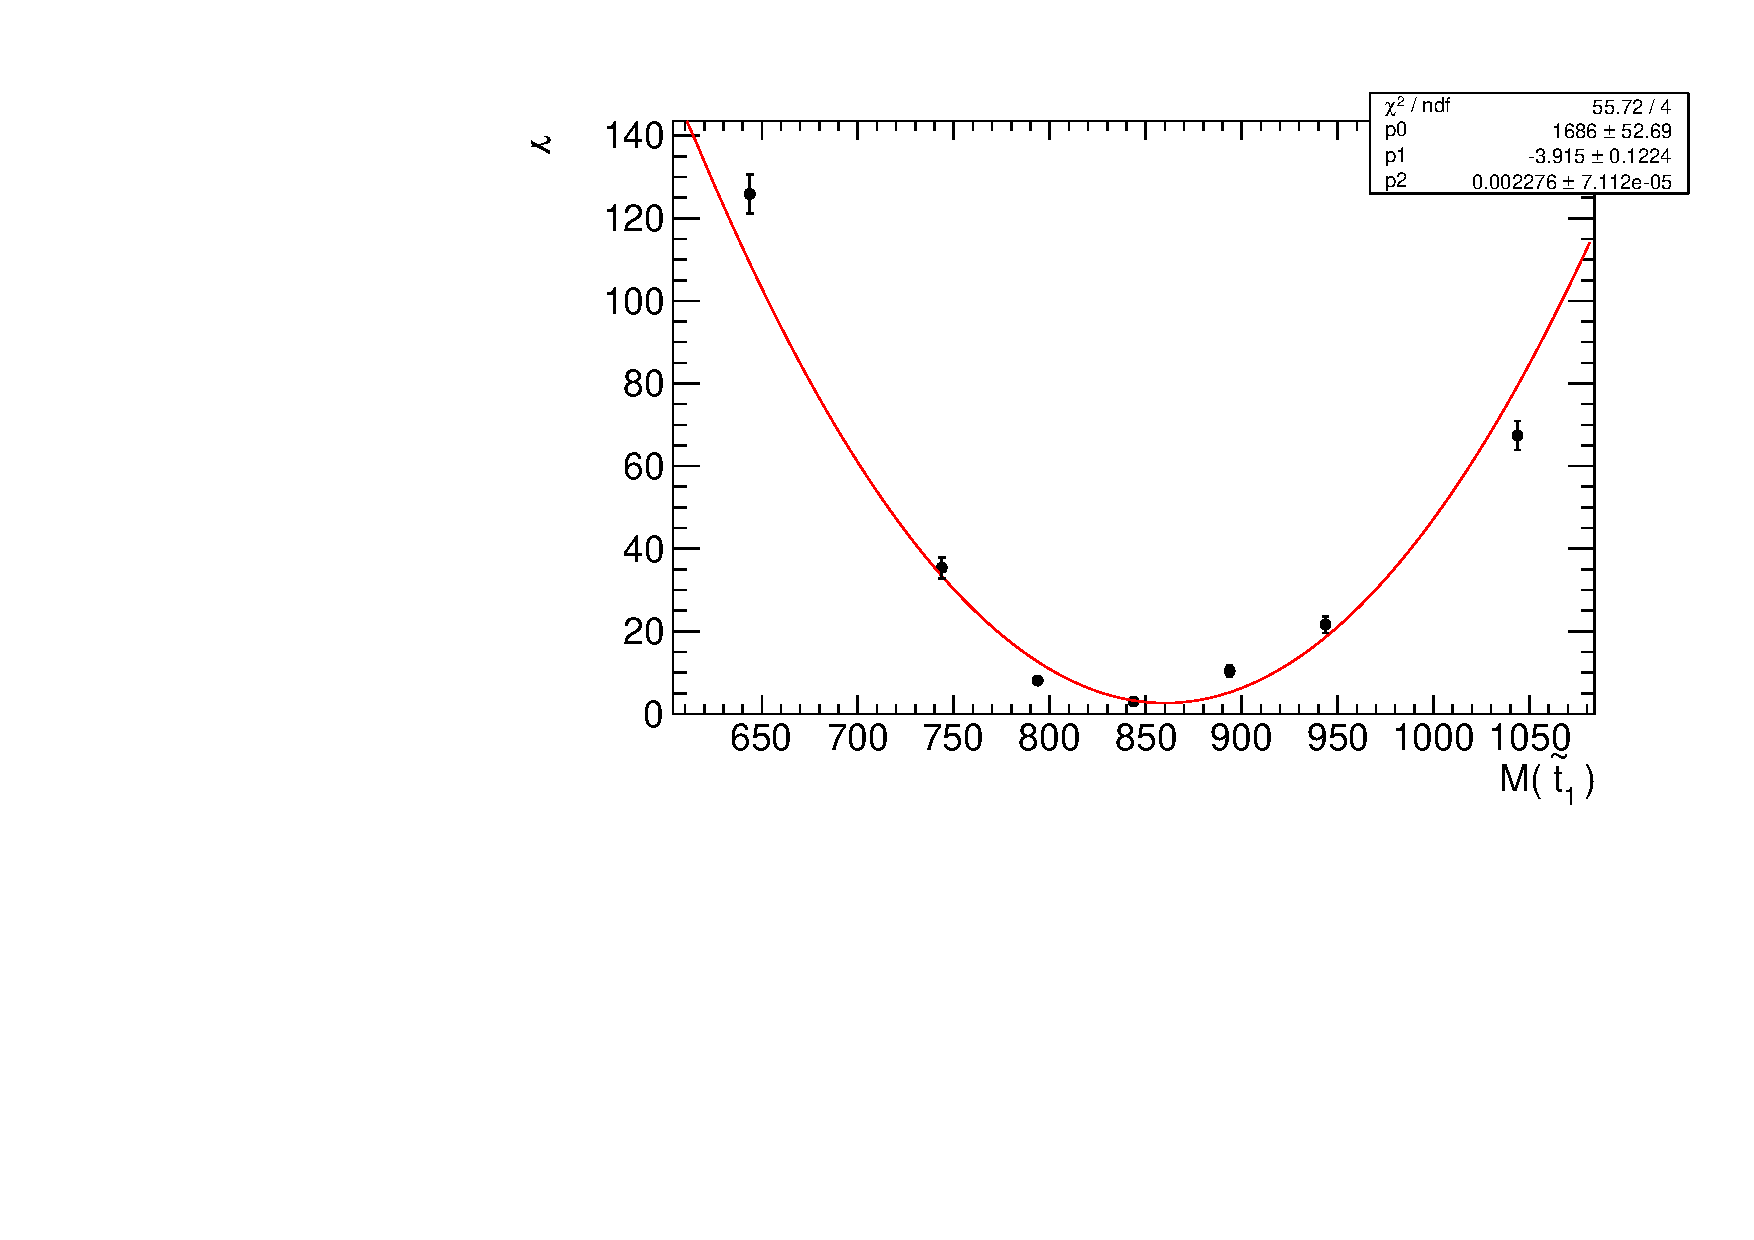
\includegraphics[width=0.7\linewidth]{{images/chisqvsmass_intlumi3000}.pdf}
  \caption{\scriptsize{The $\chi^{2}$ versus the different top squark mass templates. The minimum is at 
  860 GeV/c$^{2}$.}}
\end{figure}

In order to calculate the statistical uncertainty off the mass we employed a \textit{toy Monte Carlo Method}.

In this method, I smeared each bin of the energy spectrum of the three jets (Figure 4.12), with a Gaussian
of deviation $\sqrt{n_{data,i}}$ and mean zero. Then the mass calculation was repeated. This procedure was 
done 5000 times. The deviation of the Gaussian was chosen to have that value since $\sqrt{n_{data,i}}$
is the error of each bin content $i$. The result was an uncertainty of the mass 14 GeV.

\begin{figure}[ht!]
\centering
  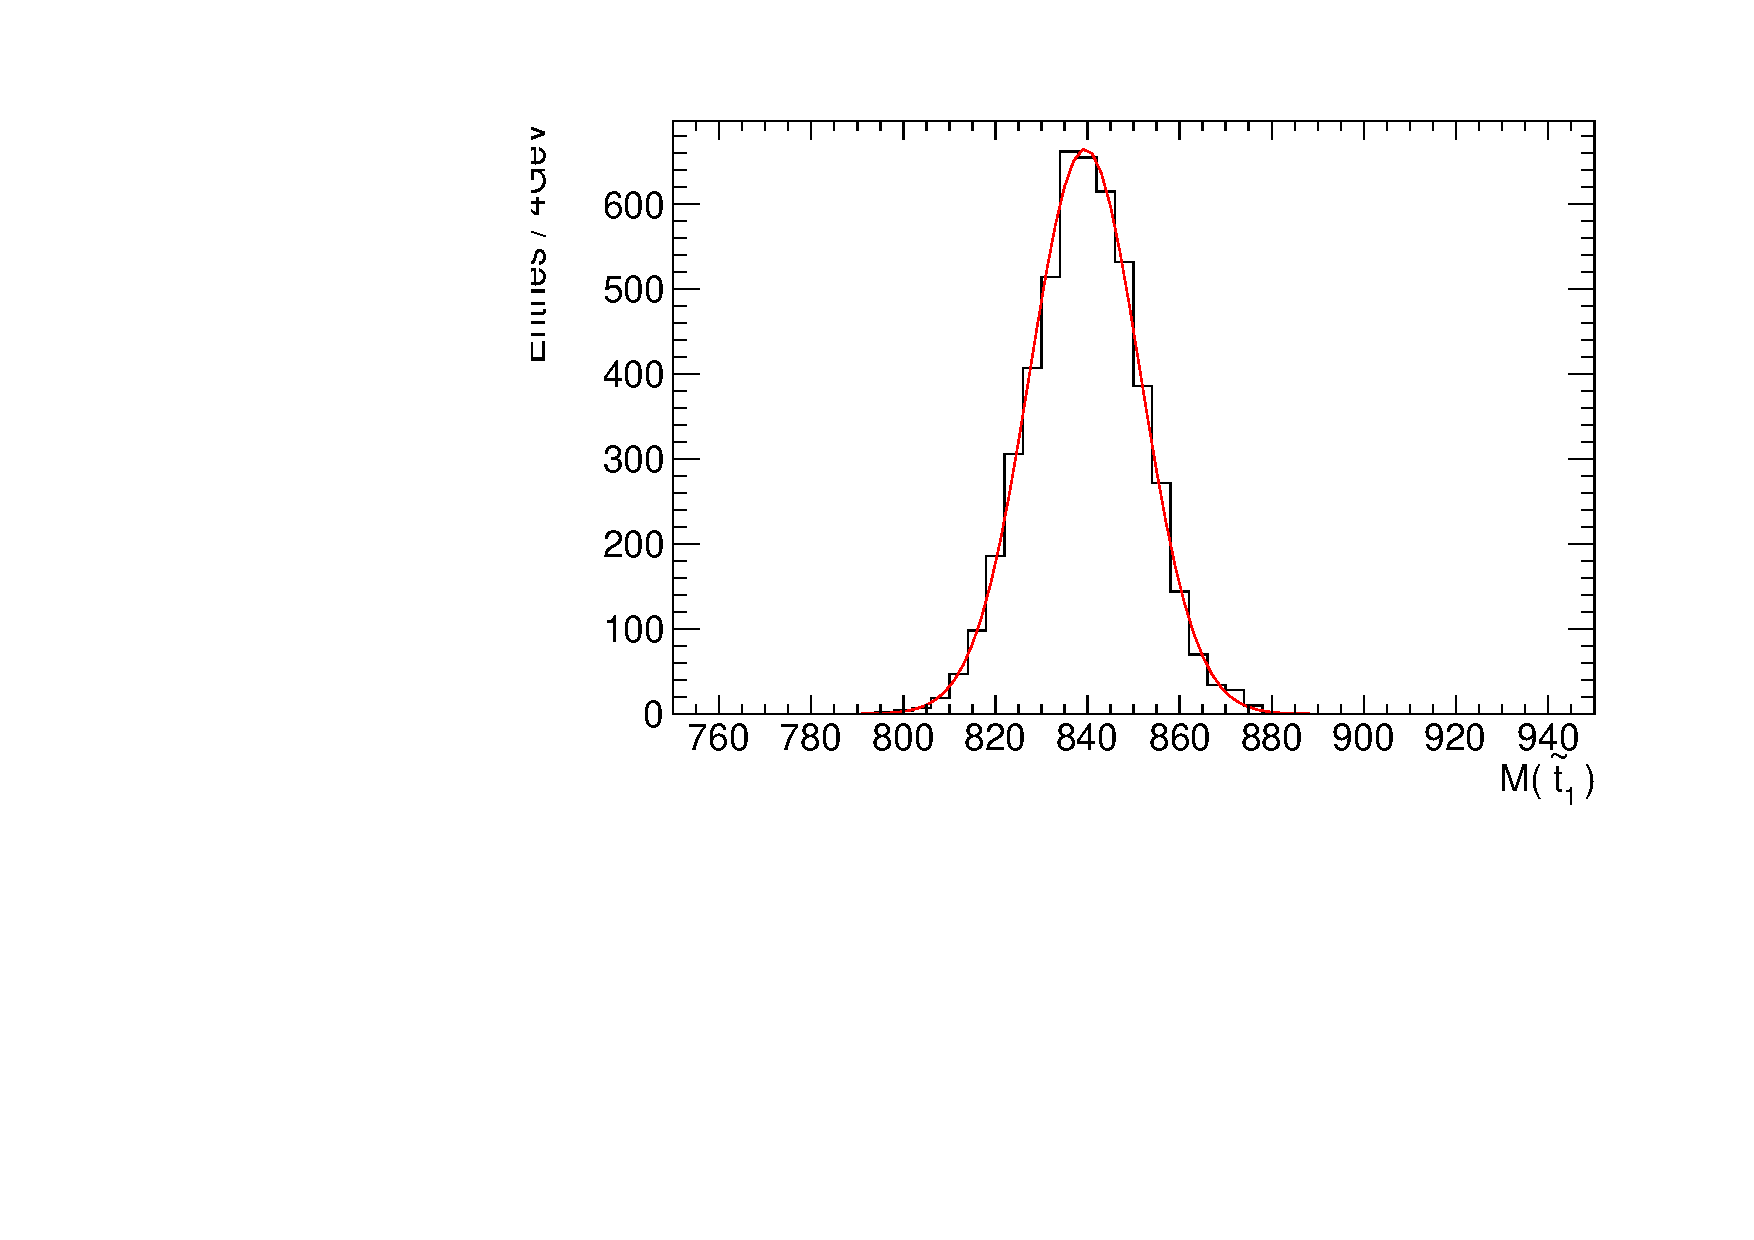
\includegraphics[width=0.7\linewidth]{{images/toyMC_intlumi3000}.pdf}
  \caption{\scriptsize{Toy Monte carlo method that yielded an uncertainty of 11 GeV.}}
\end{figure}


\newpage

\subsection{Results - Summary of the BDT method}

Using the Boosted Descision Trees and with the method of minimisation of the $\chi^{2}$ for different 
templates, I found the mass of the supersymmetric top quark to be 

\begin{equation}
 m_{\tilde{t}}=839\pm 11 \textrm{GeV}/c^{2}
\end{equation}

Although the nominal mass is $M_{nom}$= 845 GeV/$c^{2}$, my calculation is one sigma  inside this range,
taking into account the aforementioned uncertainty at CLIC for integrated luminosity 
$\mathcal{L}_{int}$=3000 fb$^{-1}$.


\newpage

\subsection{Classification Method: \textit{Gradient Boosted Descision Trees}}

In this chapter I will describe the mass calculation for the top squark using the Gradient Boosted 
Decision Trees (GBDT) as a method of classification for discrimination between signal and background. Furthermore,
comparison will be made between BDT's and GBDT's.

\subsubsection{Background on GBDT's}

Gradient Boosting is a different method for classification. The goal, as in the BDT's, is to create a 
prediction model. The main difference from the classification method described in chapter 4.3.4 is that 
the prediction model is built in an iterative way allowing its own optimisation by the calculation of errors
using a different loss function than the one used for the BDT's.

Again like all the boosting methods, it combines a set of weak learners (for BDT it was the number of trees).
In the first phase -training phase- a rough approximation for the prediction model is made. Subsequently, the 
the error of the model and the actual expected values is calculated (residual) and it is added in the
previous model making it a slightly  better. This procedure is repeated various times until a good description
is reached. 

The name gradient comes from the observation that the residuals that each time are added are just the 
negative gradient of a squared error loss function~\cite{hoecker2007tmva}. The mathematical formulation of 
both BDT's and GBDT's lies beyond the scope of this project but can be seen in~\cite{schapire1999brief},
~\cite{hoecker2007tmva}.


\subsubsection{Training and testing phase}

In this part of the procedure I "fed" the TMVA with the exact same variables as I did for the BDT's and 
imposed the exact same preselection cuts. The purpose of this is to make a comparison of the two methods in 
the end. For this method 1000 trees were employed.

The preselection cuts were:

\begin{itemize}
 \item $E_{visible} <$ 2 TeV
 \item $E_{top1,2} <$ 1.2 TeV
\end{itemize}

The list of the input variables can be seen in chapter 4.3.4 (p.16).

Based again, to the graph that has the efficiency vs the $cut_{GBDT}$, the chosen value for the cut was the one
that maximised the statistical significance $\frac{S}{\sqrt{S+B}}$, where $S$ is the signal and $B$ is the 
background: $cut_{GBDT}=-0.0606$. It needs to be noted that the statistical significance achieved through
this method is almost one point higher than that of the BDT method of classification.

\begin{figure}[ht!]
\centering
  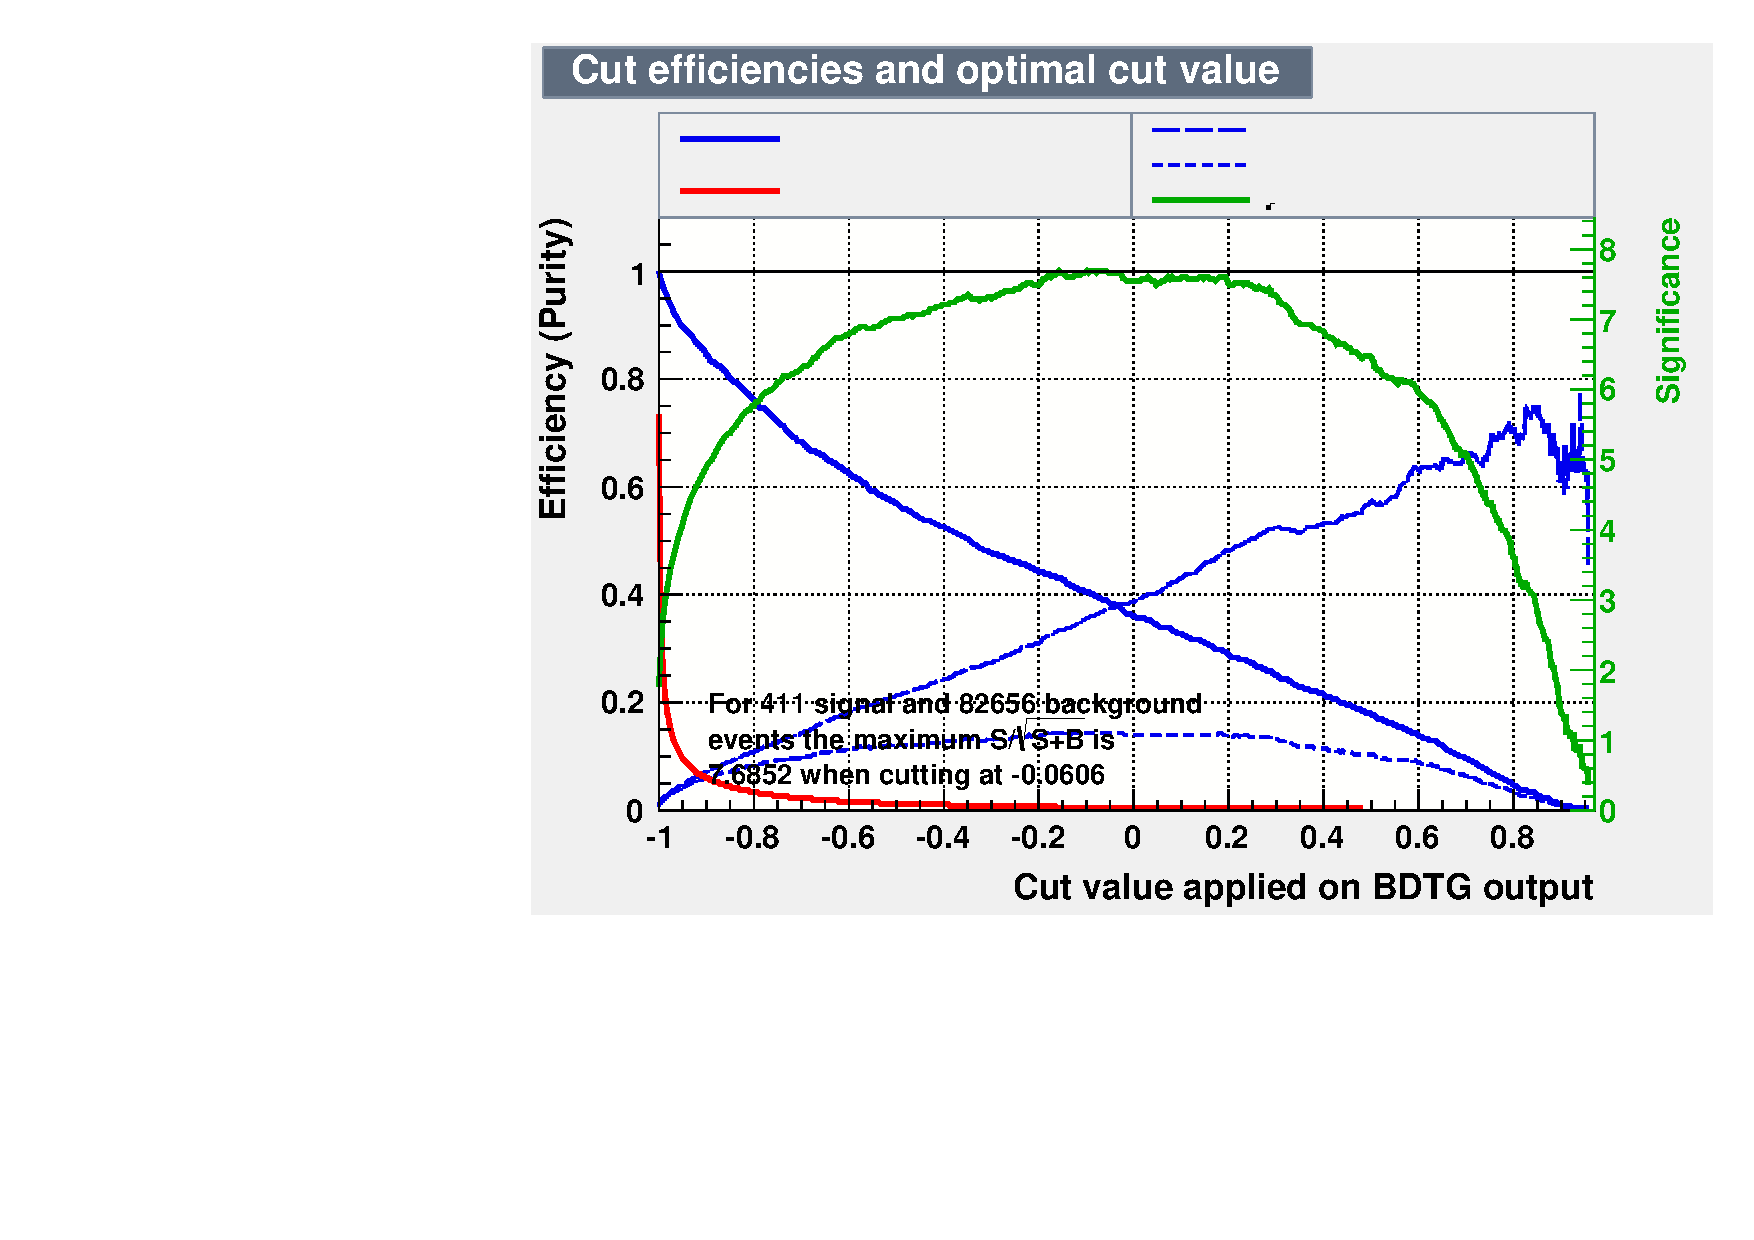
\includegraphics[width=0.7\linewidth]{{images/cutefficiency_bdtg_new}.pdf}
  \caption{\scriptsize{The green line represents the statistical significance $\frac{S}{\sqrt{S+B}}$ where as it can be
  seen it reaches the greatest value at -0.0606. The cut is also known as descision boundary and defines the
  critical region.}}
\end{figure}

The variables that TMVA found most important are exactly the same with those of the BDT method, namely:

\begin{enumerate}
 \item $\theta_{miss}$ : the polar angle of the missing momentum of the jets.
 \item $p_{T}$ : the missing transverse momentum.
 \item $\Delta \phi$ : the angle between the reconstructed tops.
 \item $cos\theta_{top}$.
\end{enumerate}

In the following stacked histogram can be seen the post GBDT reduction of background and in the table 
above, the number of events that passed (for both signal and background) are denoted.

\newpage


\begin{figure}[ht!]
\centering
  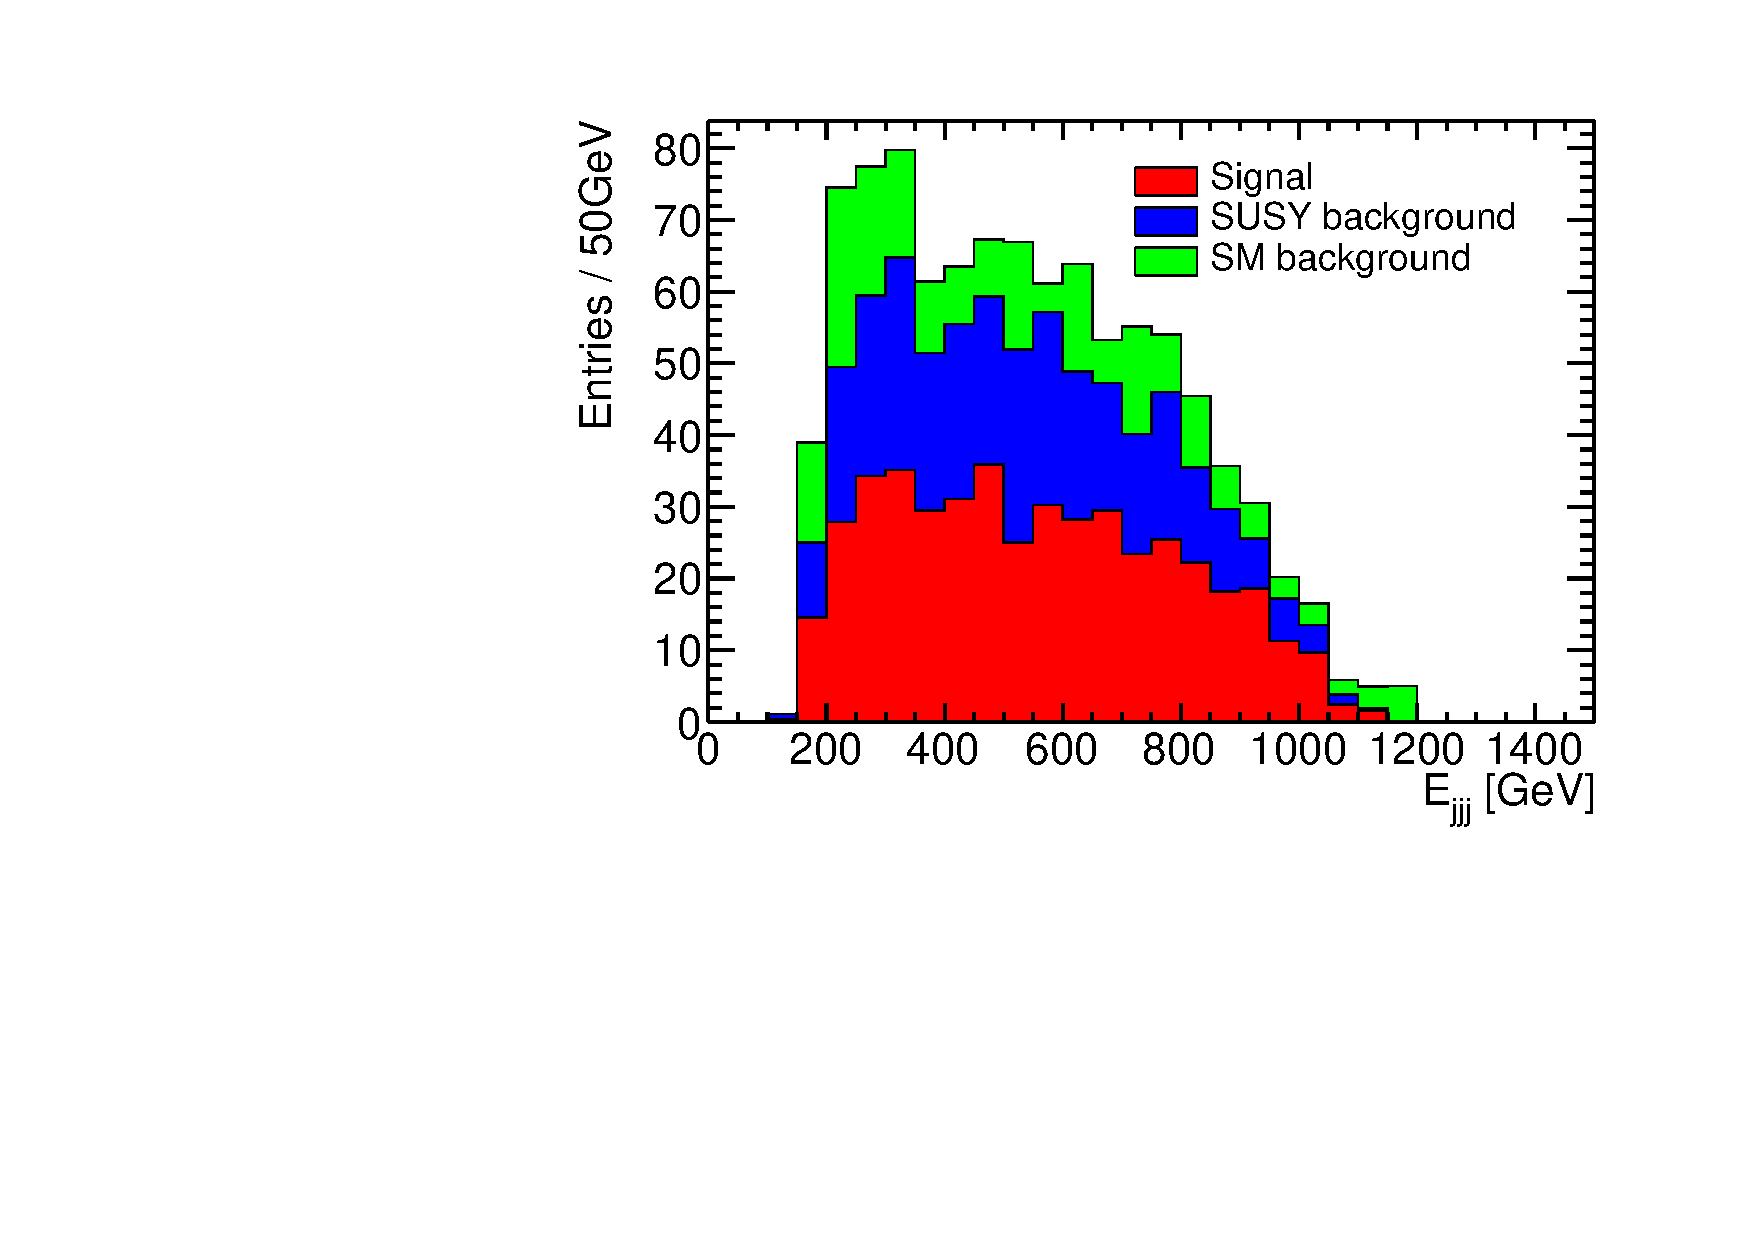
\includegraphics[width=0.7\linewidth]{{images/postbdtcut_bdtg_3000}.pdf}
  \caption{\scriptsize{Energy of the three jets after the $cut_{GBDT}$.}}
\end{figure}

\begin{table}
\centering % used for centering table
\begin{tabular}{||c | c | c | c||} % centered columns (4 columns)
\hline %inserts double horizontal lines
       GBDT      &Before TMVA ($N_{events}$)  & After TMVA ($N_{events}$) & $\%$  \\ \hline % inserts single horizontal line
Signal           & 3005     & 455       & 15 \\
SUSY background  & 17628    &  330      & 1.8 \\
SM background    & 113494   &  198      &  0.1 \\  
\hline
 %inserts single line
\end{tabular}
\label{table:nonlin} % is used to refer this table in the text
\end{table}



\begin{figure}[!hb]
\centering
  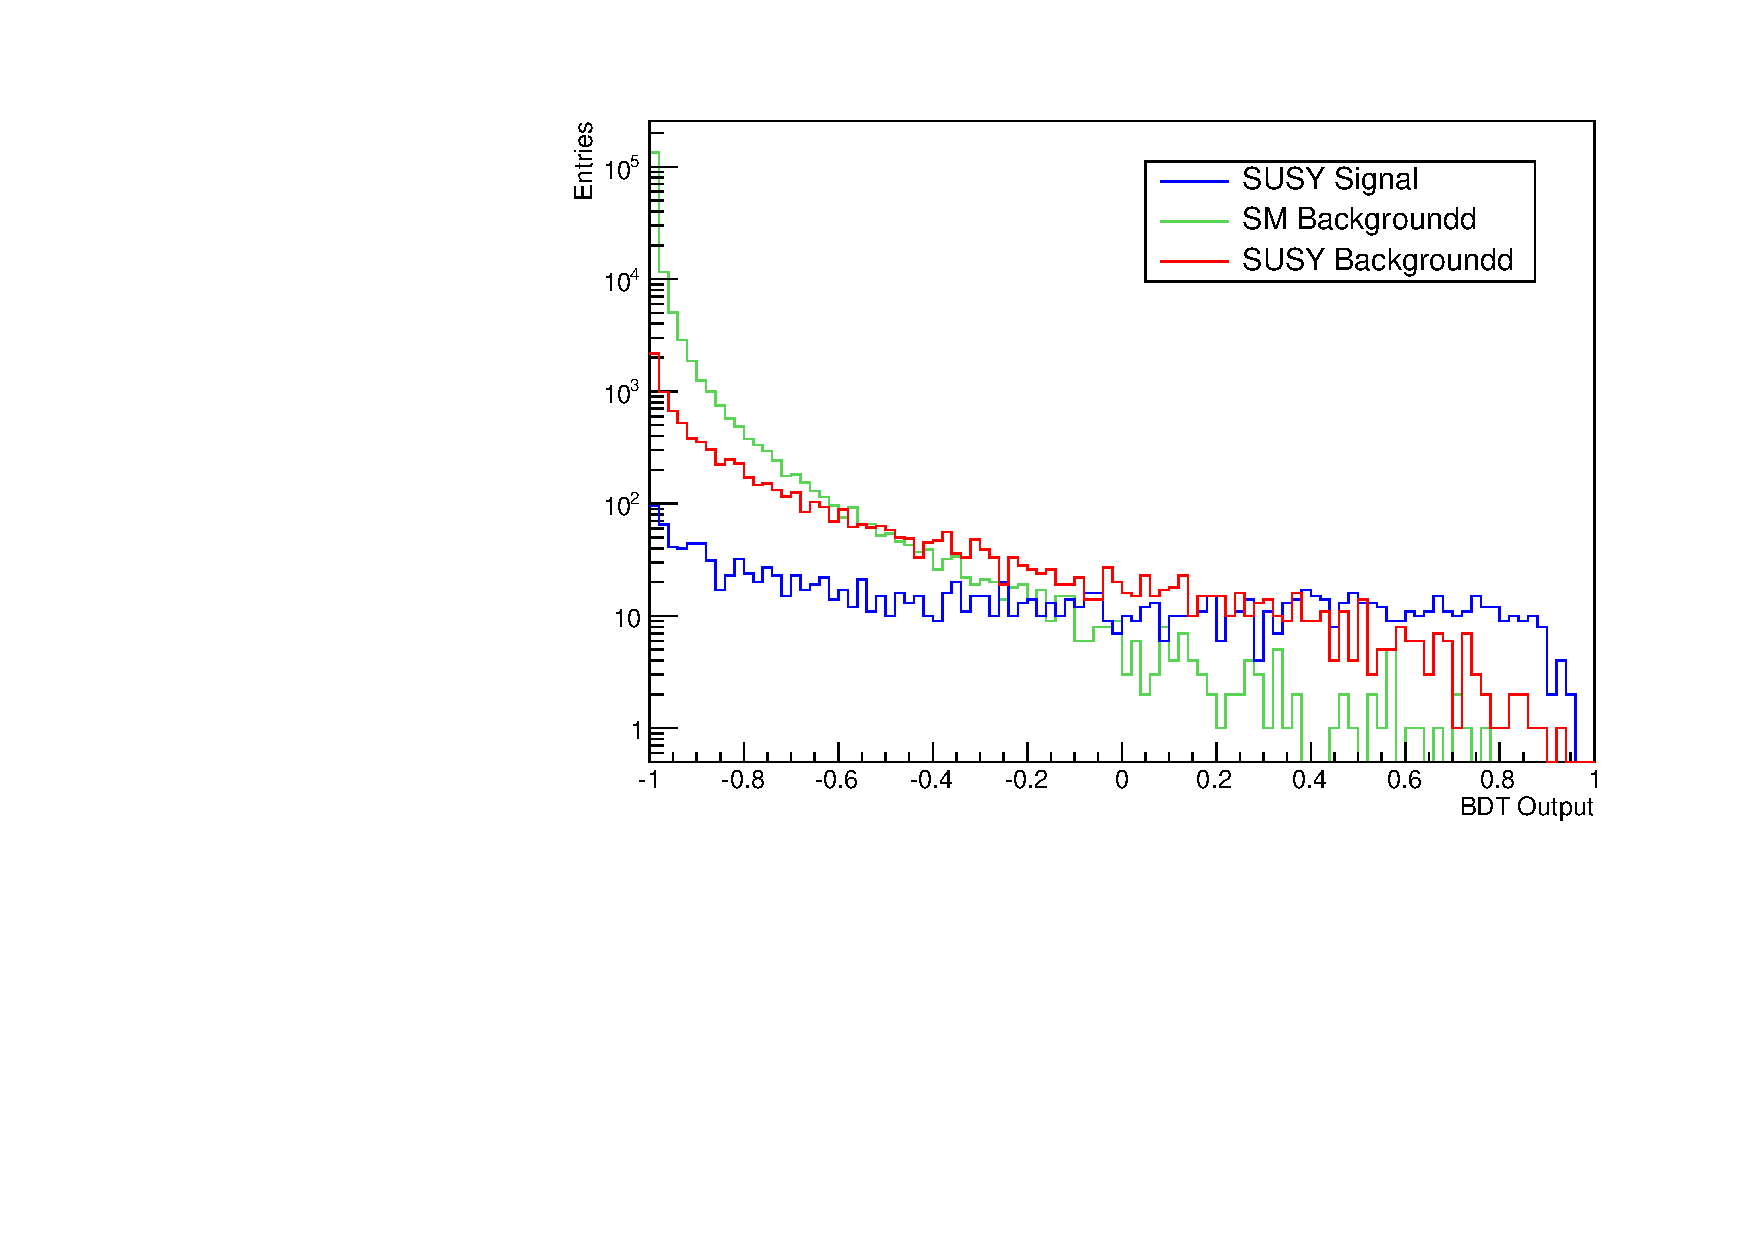
\includegraphics[width=0.7\linewidth]{{images/GBDT_output}.pdf}
  \caption{\scriptsize{The GBDT output for the signal (blue), SUSY background (red) and SM background 
  (green).}}
\end{figure}






\newpage

The above histograms show the effciency for both backgrounds whereas the one below, for the signal.
\begin{figure}
\begin{minipage}[c]{0.6\linewidth}
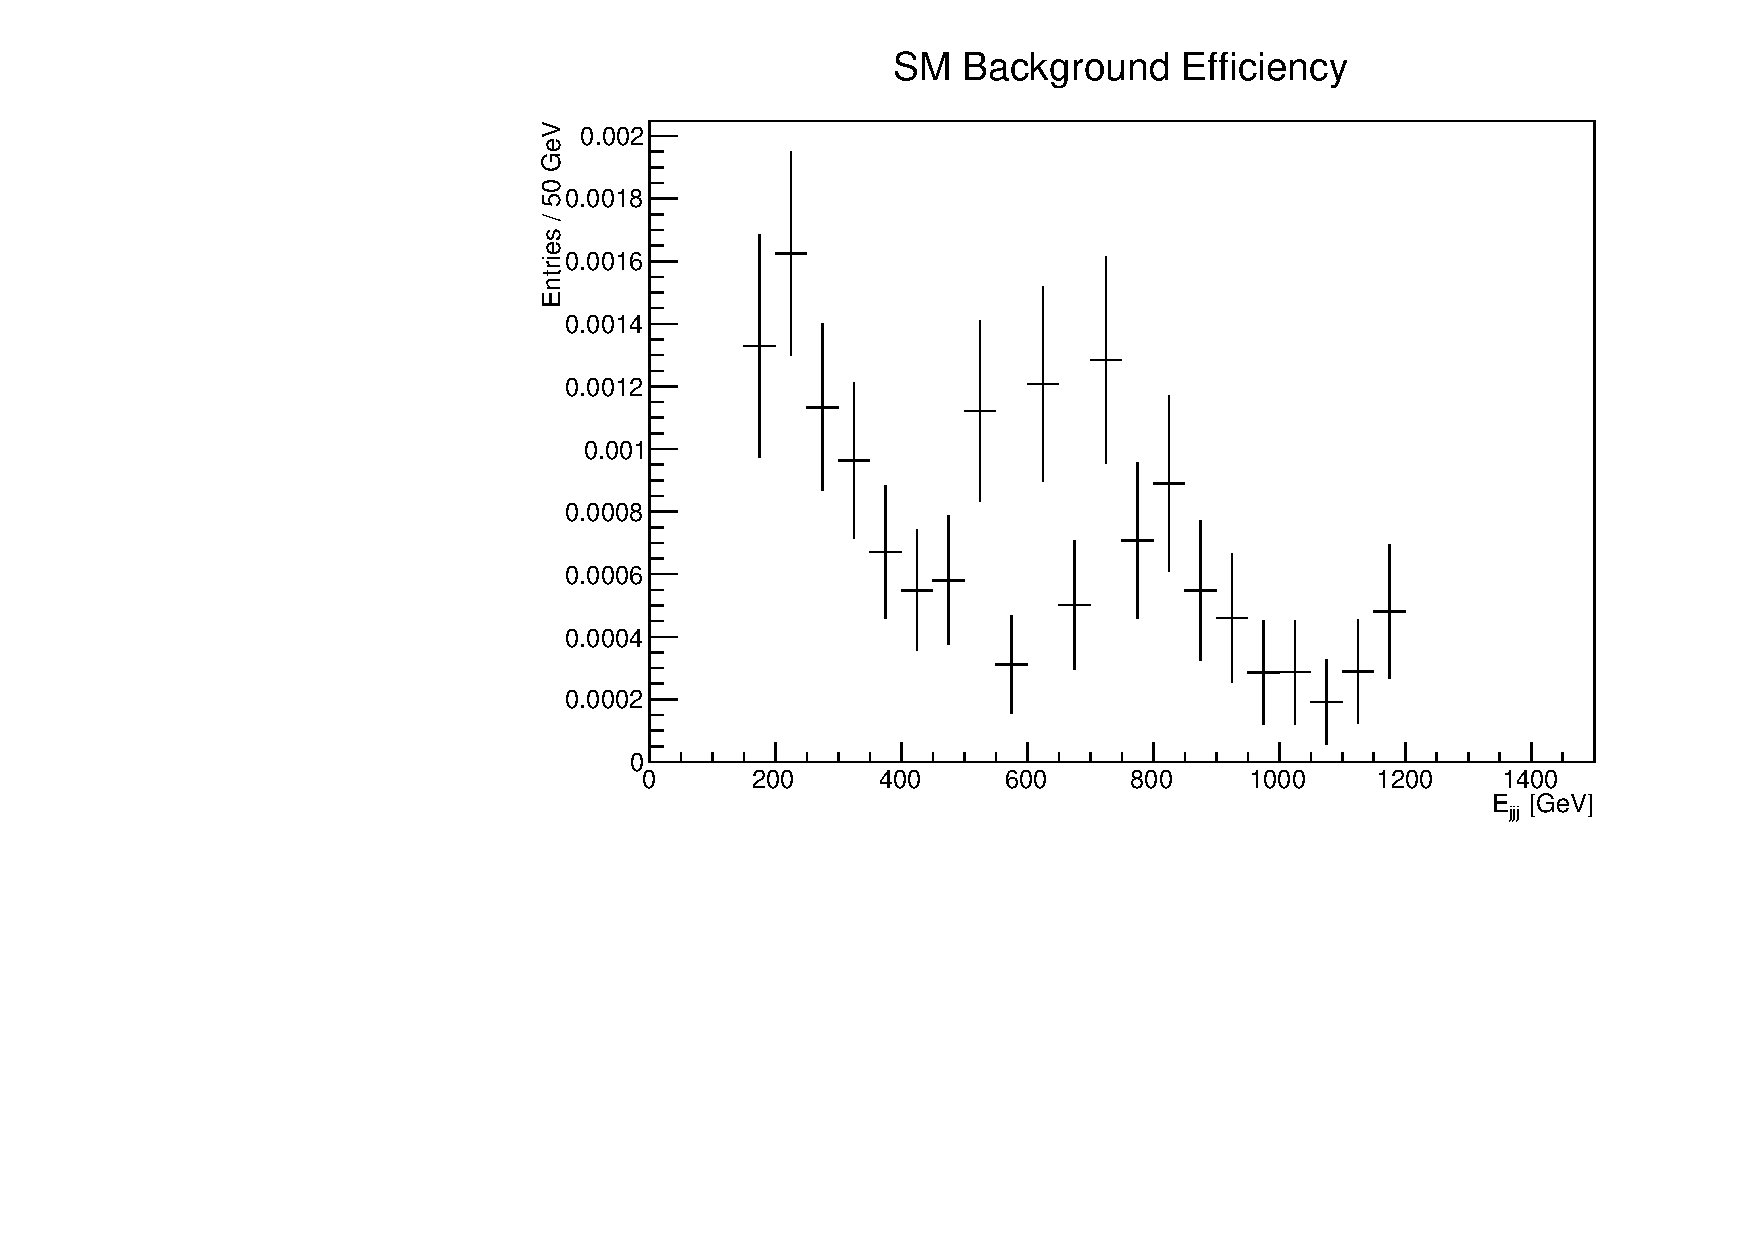
\includegraphics[width=\linewidth]{{images/ratio_plot_SMbackground_witherrors_gbdt}.pdf}
\caption{\scriptsize{The Standard Model Background Efficiency for the GBDT method.}}
\end{minipage}
\hfill
\begin{minipage}[c]{0.6\linewidth}
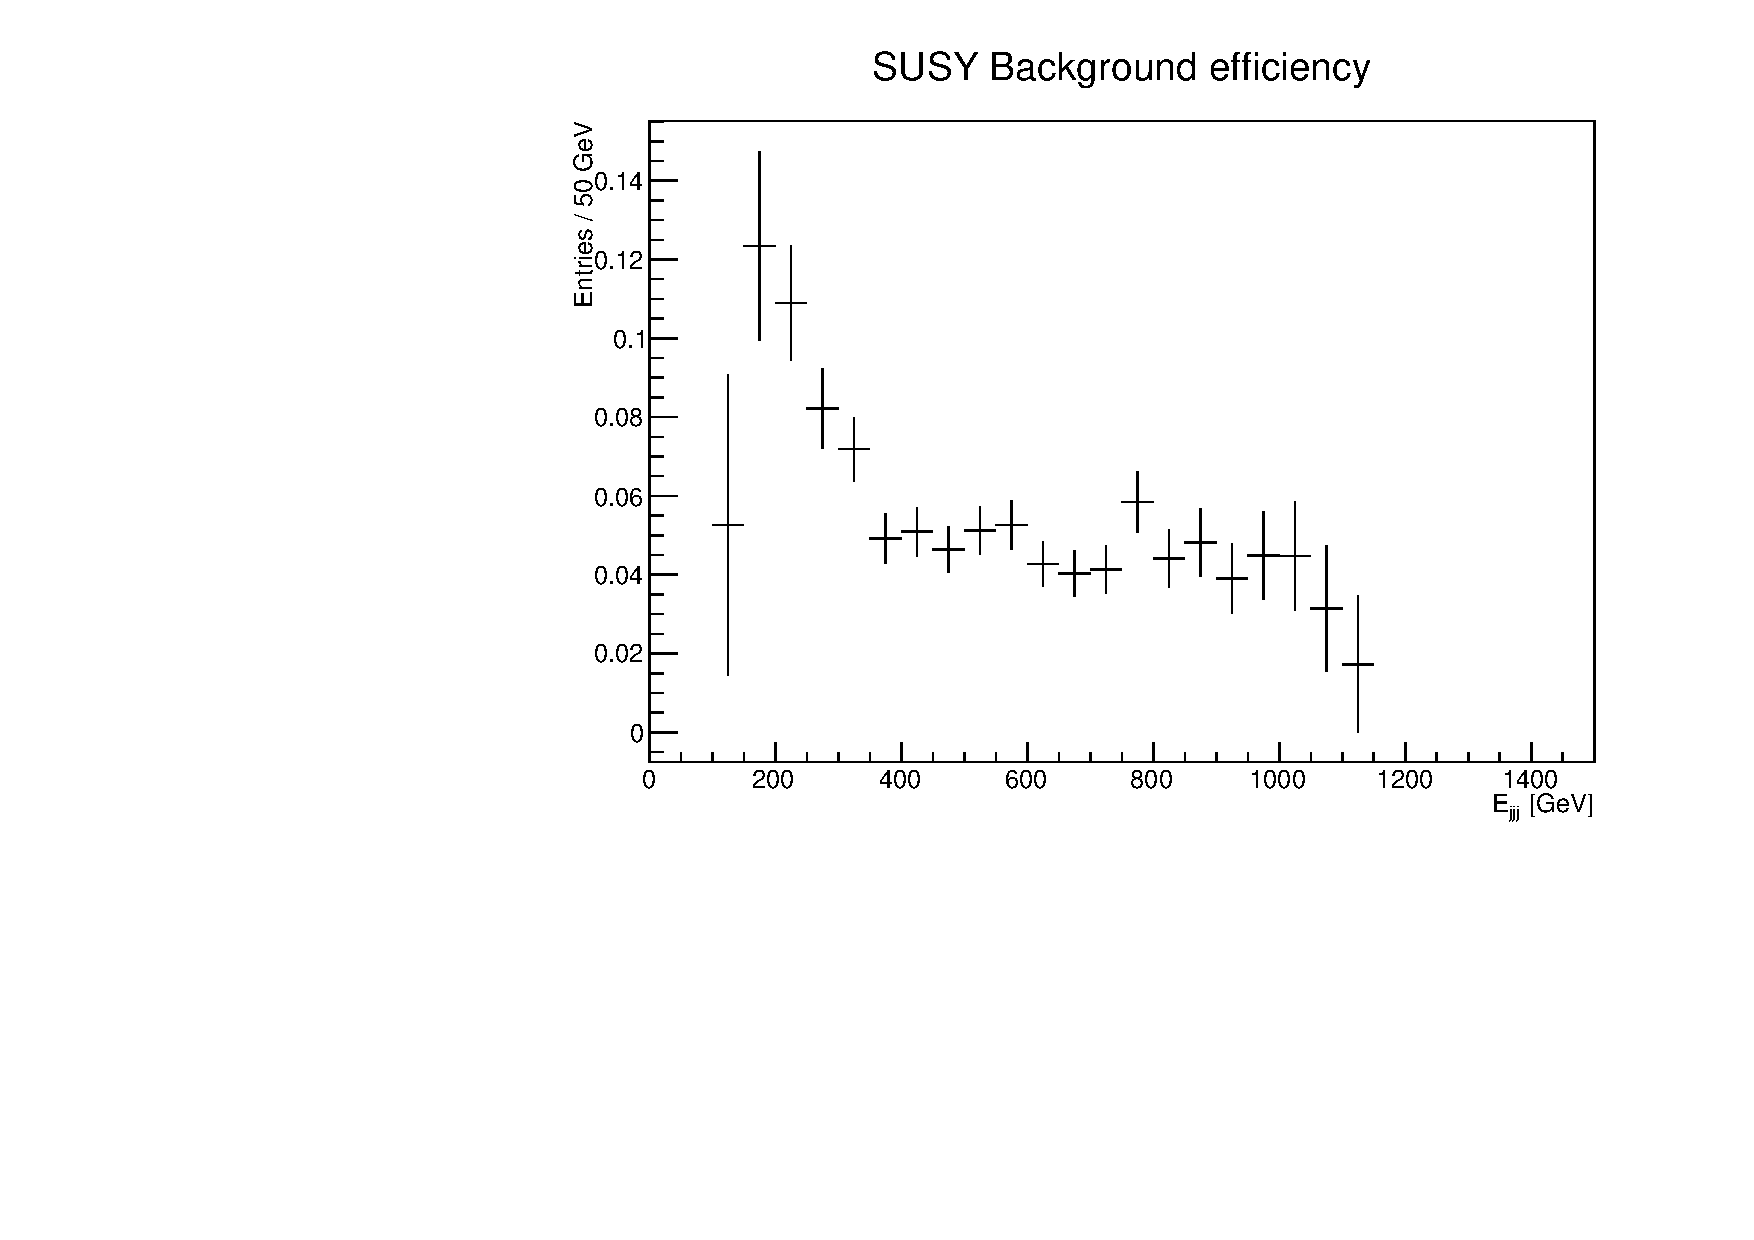
\includegraphics[width=\linewidth]{{images/ratio_plot_susybg_witherrors_gbdt}.pdf}
\caption{\scriptsize{The SUSY Background Efficiency for the GBDT method.}}
\end{minipage}
\end{figure}



\begin{figure}[!hb]
\centering
  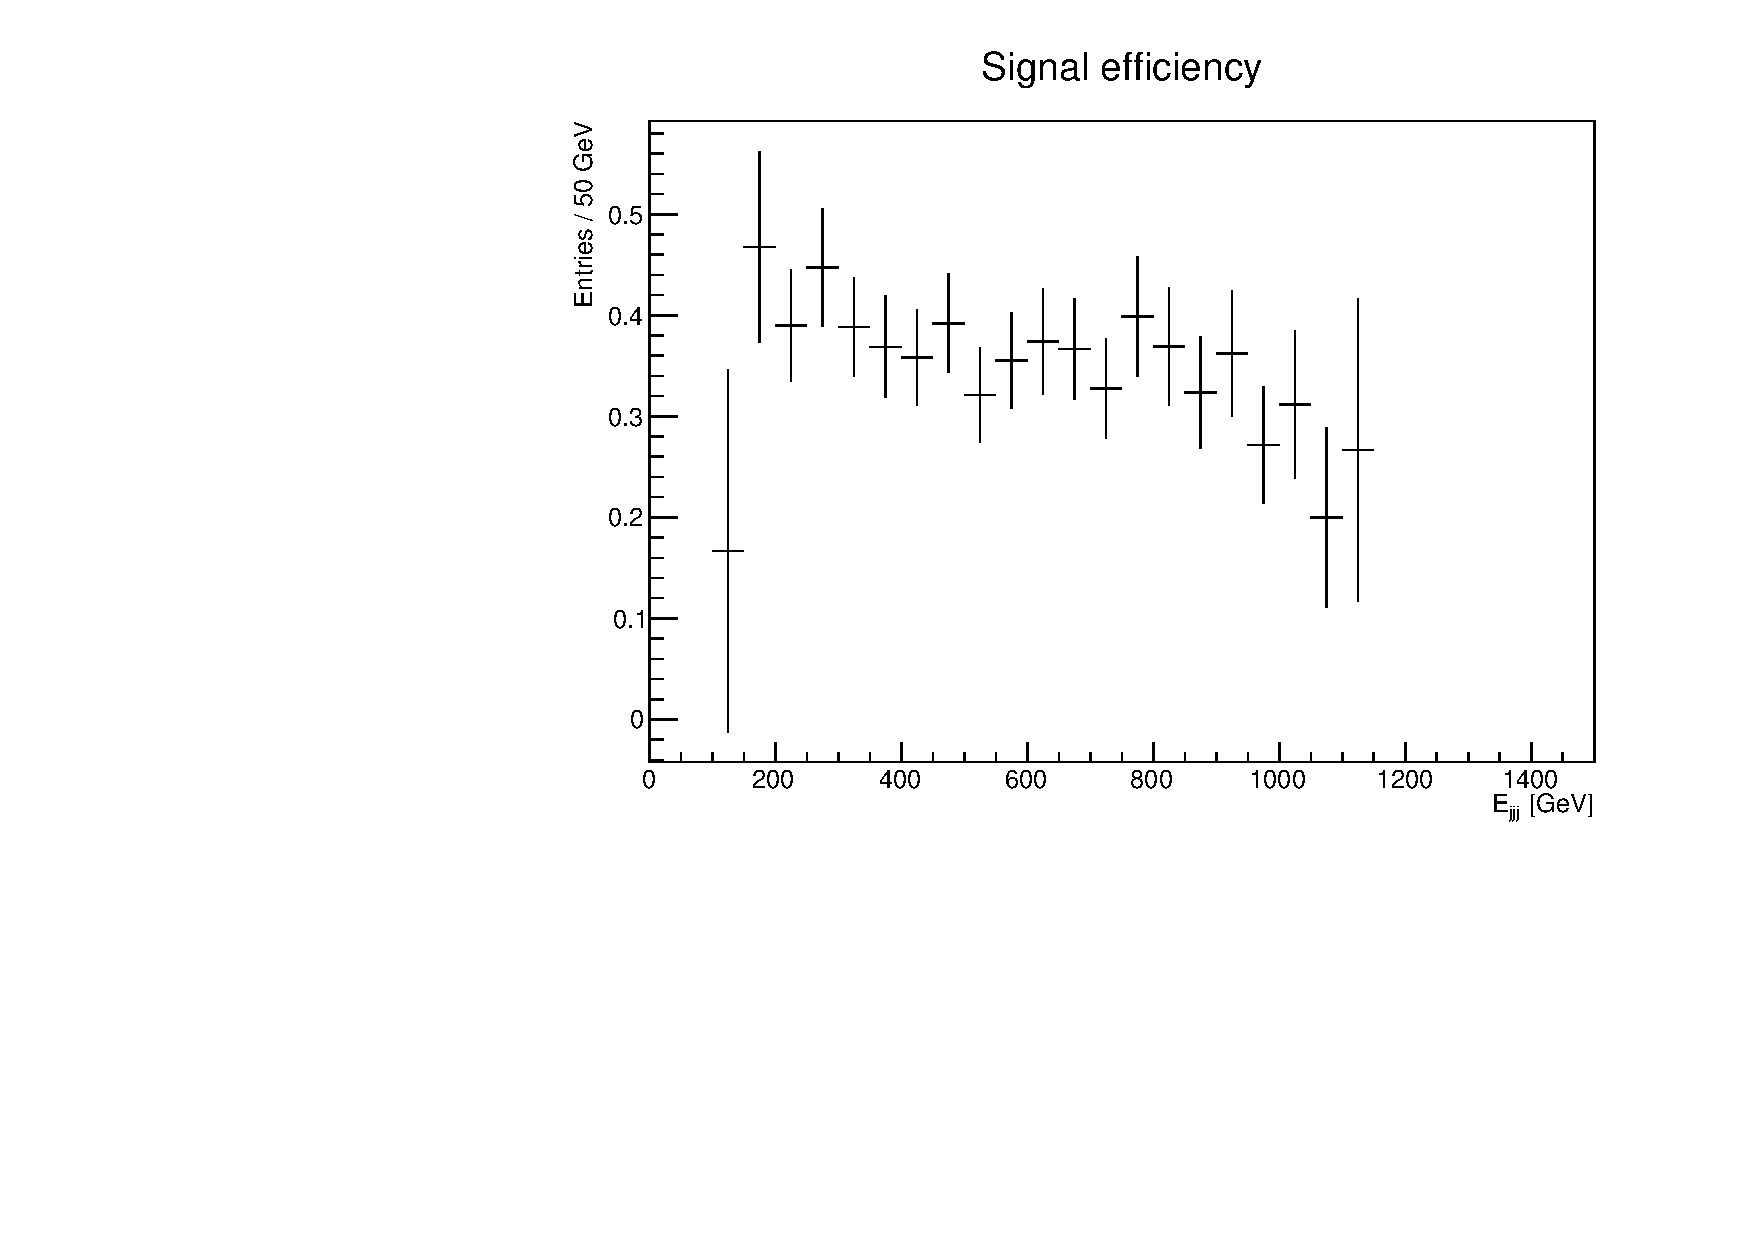
\includegraphics[width=0.7\linewidth]{{images/ratio_plot_witherrors_gbdt}.pdf}
  \caption{\scriptsize{The signal efficiency for the GBDT method.}}
\end{figure}


Using again the method of minimisation of the $\chi^{2}$ for different templates (table in p.22) of the top 
squark mass (formula 4.9), I calculated the mass to be:
\begin{equation}
 m_{\tilde{t}}=811\quad \textrm{GeV}
\end{equation}

again using a toy Monte Carlo method I smeared each bin of the energy spectrum of the three jets with a 
Gaussian of deviation $\sqrt{n_{data}}$ and mean zero, and I repeated the mass calculation. This procedure
was done 5000 times. The resulting uncertainty was 19 GeV. 

Both calculations can be seen in the following graphs where in the first the minimisation of the $\chi^{2}$
can be seen and in the second the calculation of the uncertainty.


\begin{figure}[!hb]
\centering
  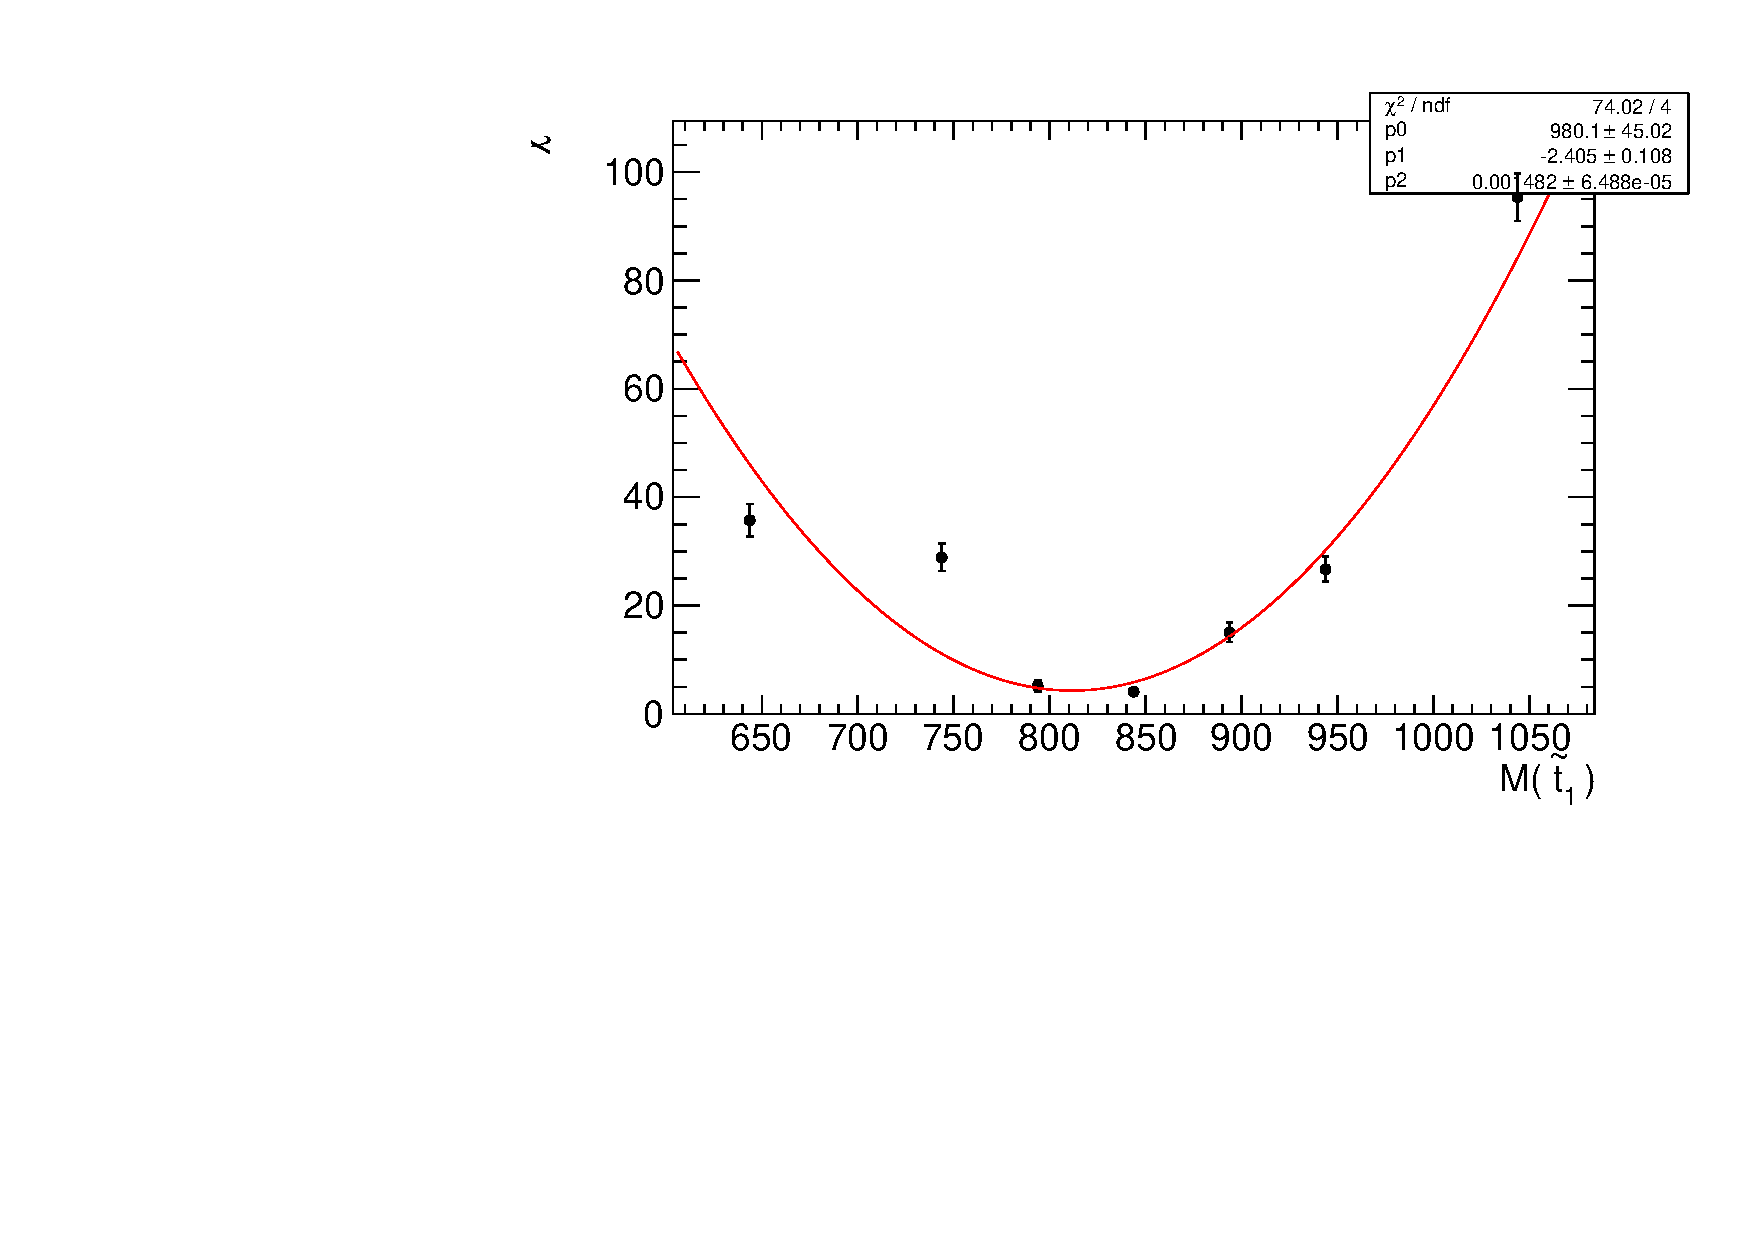
\includegraphics[width=0.7\linewidth]{{images/chisqvsmass_gbdt}.pdf}
  \caption{\scriptsize{The $\chi^{2}$ versus the different mass templates. The minimum is at 811 GeV/$c^{2}$.}}
\end{figure}

\begin{figure}[!hb]
\centering
  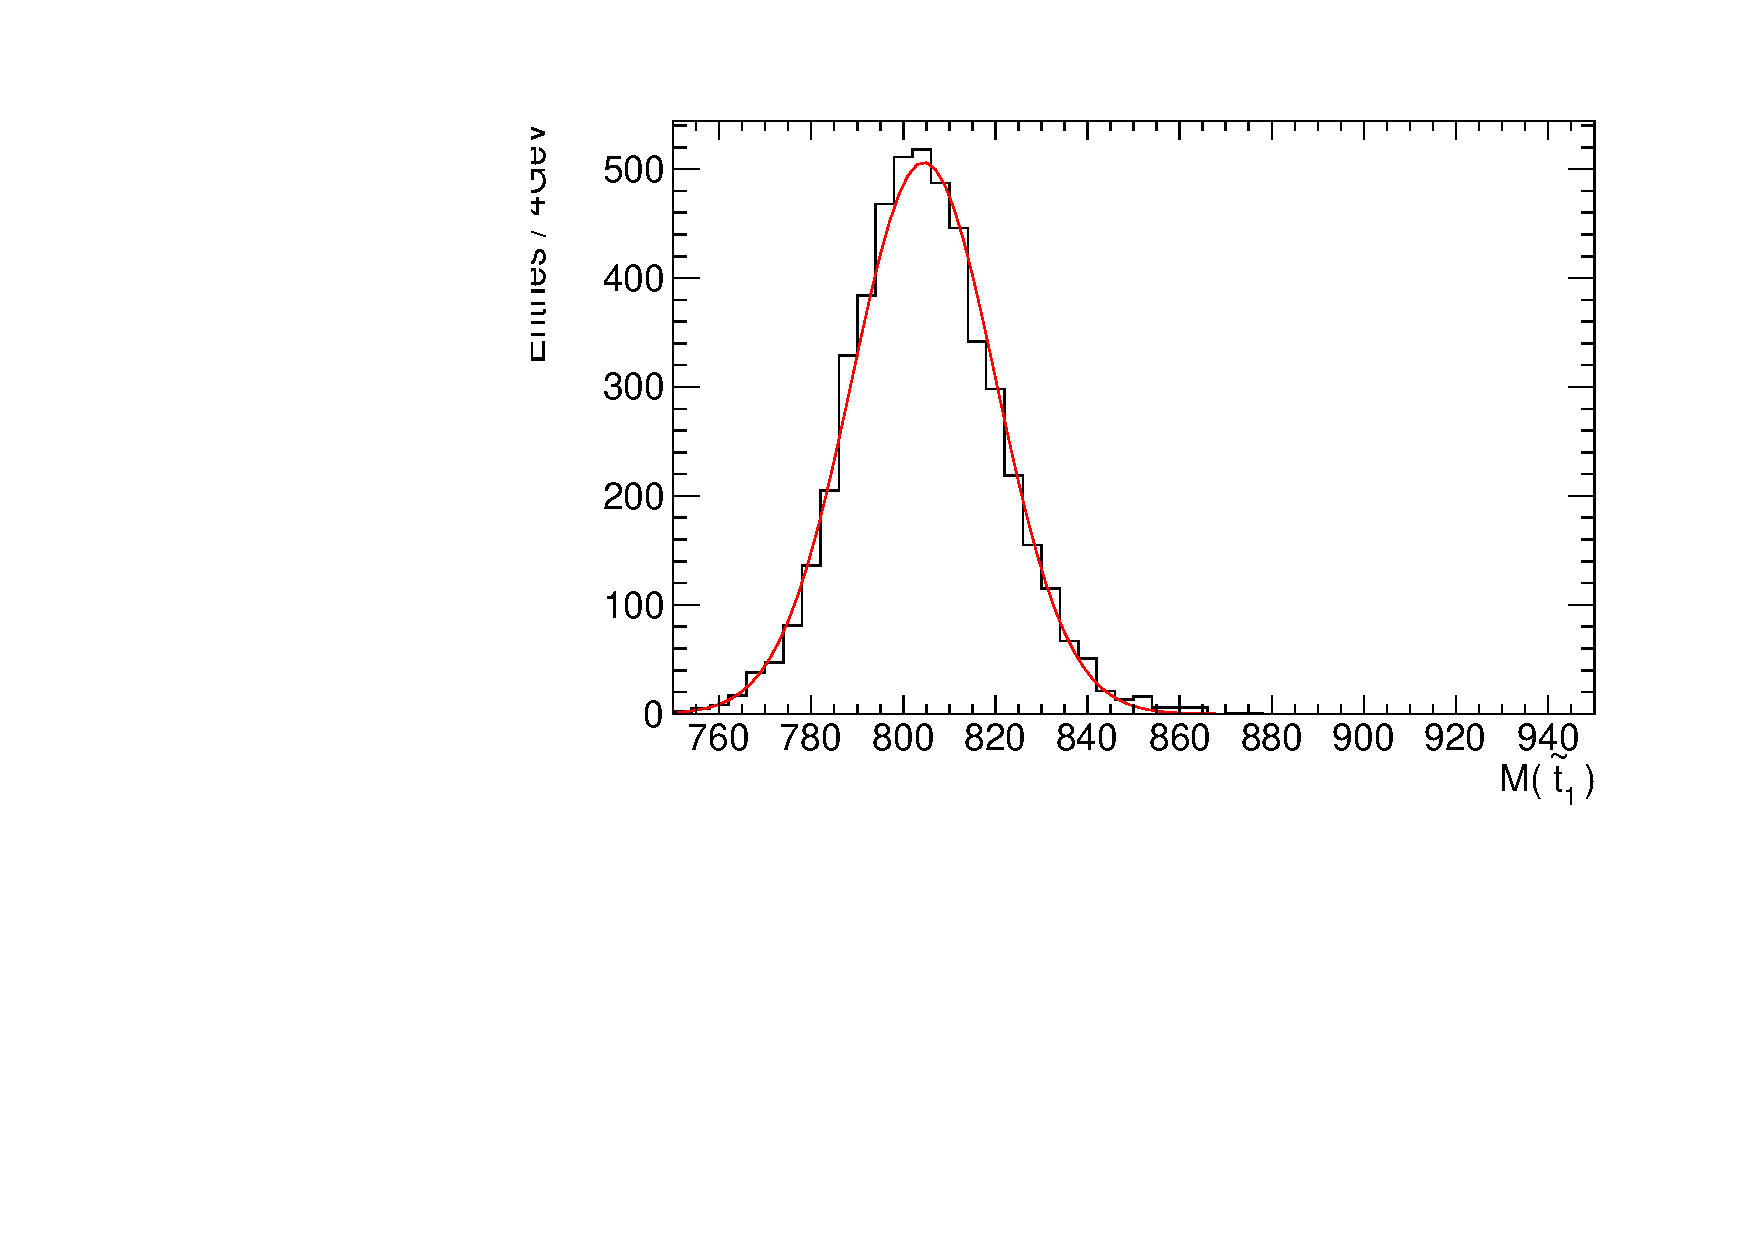
\includegraphics[width=0.7\linewidth]{{images/toyMC_gbdt}.pdf}
  \caption{\scriptsize{The resulting uncertaity from the toy Monte Carlo method is 15 GeV.}}
\end{figure}

\newpage

\subsection{Results - Summary of the GBDT method}

Using the Gradient Boosted Descision Trees and with the method of minimisation of
the $\chi^{2}$ for different mass templates, I found the mass of the supersymmetric top
quark to be:

\begin{equation}
 m_{\tilde{t}}=811\pm 15 \quad \textrm{GeV}
\end{equation}

The nominal mass is $M_{nom}$ = 845 GeV/$c^{2}$, my calculation is two sigma inside this range taking into 
account the uncertainty calculated through the toy MC method at CLIC for an integrated luminosity
$\mathcal{L}_{int}$=3000 fb$^{-1}$.

\section{Comparison of BDT - GBDT methods/Results}

In this section I am going to compaire the performance as well as the results of the two methods followed in
this project.

For the BDT method I set the number of weak learners (trees) to be 1000 and the maximum depth of the tree to 
be 3. Same considarations took place also for the the GBDT method.

The following table summarises the basic characteristics of the two methods:



\begin{table}[!hb]
\centering % used for centering table
\begin{tabular}{||c | c | c | c||} % centered columns (4 columns)
\hline %inserts double horizontal lines
Method      &Stat. Efficiency &  $m_{\tilde{t}}$               &  $N_{signal}$ \\ 
\hline 
BDT         &       6.79      &  839 $\pm$ 11 GeV/$c^{2}$      &  493		\\
GBD         &       7.68      &  811 $\pm$ 15 GeV/$c^{2}$      &  455		\\
\hline
 %inserts single line
\end{tabular}
\label{table:nonlin} % is used to refer this table in the text
\end{table}


As it can be seen the GBDT method achieves higher statistical significance in comparison with the BDT method
but higher uncertainty with a difference of 4 GeV. This can be attributed to the fact that the proposed cuts 
from the TMVA are mainly addressed for particle discoveries rather than for measuring an observable. That 
means that for the optimal precision of the TMVA one has to "play" with the value of the cut -primarily
around the proposed value - in order to extract the lowest uncertainty possible for the mass calculation.
Furthermore as it can be seen in the above graph, the number of events after the TMVA cut, in the case of 
GBDT are almost 40 less. Even thought that they sound few, as a fraction they constitute 8$\%$ of the
$N_{signal}$,
number not at all negligible especially when we deal with a few hundreads of events.
Additionally another interesting thing is the importance of these 40 more events in the case of BDT.
This is cleat because in the BDT the number of events of SM background ($N_{events}$=528) 
in total are far more 
than those in the GBDT method ($N_{events}$=198), and at first sight it would be expected that the GBDT has 
better potencial than the BDT. The mass and uncertainty measurements proved to be the other way round.

Similar contradiccion produces the careful examination of the signal efficiency plots(4.8 for BDT and 4.20
for GBDT). Both of them (taking into account the errors) tend to have an almost constant trend but the 
efficiency of GBDT is higher.

Although, apart from the "cut tunning" issue, the fact that the BDT's performance is superior is is no 
new to the experimental world. From 2005, similar studies were made for the MiniBoone experiment and 
it was found that BDT's (on Adaboost mode) outperform other methods~\cite{yang2005studies}.






























\section{Some results}
Here are some results.


\section{Discussion of your results}

This section should give a picture of what you have taken out of your
project and how you can put it into context.

This section should summarise the results obtained, detail conclusions
reached, suggest future work, and changes that you would make if you
repeated the project.

\chapter{Conclusions}

This is the place to put your conclusions about your work. You can
split it into different sections if appropriate. You may want to include
a section of future work which could be carried out to continue your
research.

The conclusion section should be at least one page long, preferably 2
pages, but not much longer.

\appendix
% the appendix command just changes heading styles for appendices.

\chapter{Stuff that's too detailed}

Appendices should contain all the material which is considered too
detailed to be included in the main body of the text, but which is
important enough to be included in the thesis.

Perhaps this is a good place to mention \BibTeX.

You can do references in the simple way explained in the introduction,
or you can use \BibTeX.


\section{\BibTeX}
\label{sec:bibtex}

It is convenient to use \BibTeX\ to compile your bibliography.  First
you need to create a .bib file e.g.  you may call it ref.bib Then you
can put all your references into the file with entries such as
\begin{verbatim}
@Book{ob:bornwolf,
     author = "Born, M and Wolf, E",
     title  = "Principles of Optics",
     publisher = "Cambridge University Press",
     year = 1999,
     edition = {7th},
}

@Article{jr:ashkin,
Author = {A. Ashkin and J.M. Dziedzic and J.E. Bjorkholm and S. Chu},
Title = "Observation of a single beam gradient force optical tap for 
dielectric particles",
Journal = "Optics Letters",
Volume = 11,
Pages = "288-290",
Year = 1986}

@INPROCEEDINGS{seger,
 author = {J. Seger and H.J. Brockman},
 title = {What is bet-hedging?},
 editors={P.H. Harvey and L. Partridge},
 booktitle = {Oxford Surveys in Evolutionary Biology},
 year={1987},
 page={18},
 publisher={Oxford University Press},
 place={Oxford}}
\end{verbatim}
for a book, an article in a journal or an article in a proceedings volume
respectively.

Inside your \LaTeX\ file
you should include 
\begin{verbatim}
\bibliographystyle{unsrt}                      
and
\bibliography{ref}
\end{verbatim}
The first command determines the reference style, here plain and 
unsorted. With this referencing style 
a numerical referencing system (which is now the most
common in physics literature) is used and the numbering of references
will be the order in which they appear in the document. Alternatively, 
you could use
a customised `style file' but there is no real need.  The second
command just inputs your .bib file Note that only the references cited
in the text will appear in the bibliography so you can have spare
references in your .bib file.


You use the name you have given to an entry (e.g.
for the book example above the name is ob:bornwolf)
to cite the relevant article
by using the cite command in your \LaTeX\ file e.g. \cite{ob:bornwolf}



\section{Producing your documents using \texttt{pdflatex}}

To use pdflatex your figures need to be in pdf format.  You can convert almost any image file to pdf using \texttt{convert}.  e.g. \texttt{convert myfigure.png myfigure.pdf}.

The first time you should type:
\begin{verbatim}
  pdflatex ProjectReport
  bibtex ProjectReport
  pdflatex ProjectReport
  pdflatex ProjectReport
\end{verbatim} 
This first time you run\texttt{pdflatex} it will produce a
\texttt{ProjectReport.aux}.  The \BibTeX\ command reads in the
bibliography file and makes the files \texttt{ProjectReport.bbl} and
\texttt{ProjectReport.blg} files.  These files are read in the next
\texttt{pdflatex} command, but you'll still have ``undefined
cross-reference'' errors which are sorted out by the last
\texttt{pdflatex} command.

Subsequently, you should only need to do one (or two)
\texttt{pdflatex}s, or \texttt{pdfbibtex} followed by
\texttt{pdflatex} twice if you change any references.

\vspace{5mm} You may also use plain \texttt{latex} instead of
\texttt{pdflatex}.  This requires you to use postscript graphics
instead of pdf.




\chapter{Stuff that won't be read by anyone}

Some people include in their thesis a lot of detail, particularly lots
of tables containing raw results, figures of intermediate results, or
computer code which no-one will ever read. You should be careful that
anything like this you include should contain some element of
uniqueness which justifies its inclusion.


\newpage

\bibliographystyle{unsrt}
\bibliography{MSc_dissertation}


\end{document}

